\documentclass[a4paper,10pt]{report}
\usepackage[cm]{fullpage}
\usepackage[utf8]{inputenc}
%\usepackage[italian]{babel}
\usepackage{amsmath}
\usepackage{amsthm}
\usepackage{amssymb}
\usepackage{appendix}
\usepackage{booktabs}
\usepackage[table]{xcolor}
\usepackage{amssymb}
\usepackage{multirow}
\usepackage{fullpage}
\usepackage{float}
\usepackage{wrapfig}
\usepackage{subfig}
\usepackage{graphicx}
\usepackage{listings}
\usepackage{color}
\usepackage{textcomp}

\usepackage{hyperref}

\definecolor{listinggray}{gray}{0.9}
%\definecolor{lbcolor}{rgb}{0.9,0.9,0.9}

\addtolength{\voffset}{-10pt}

\hypersetup{colorlinks=false}
 
\lstset{
%	backgroundcolor=\color{lbcolor},
	tabsize=4,
%	rulecolor=,
	language=python,
        basicstyle=\scriptsize,
        upquote=true,
        aboveskip={1.5\baselineskip},
        columns=fixed,
        showstringspaces=false,
        extendedchars=true,
        breaklines=true,
        prebreak = \raisebox{0ex}[0ex][0ex]{\ensuremath{\hookleftarrow}},
%        frame=single,
        showtabs=false,
        showspaces=false,
        showstringspaces=false,
        identifierstyle=\ttfamily,
        keywordstyle=\color[rgb]{0,0,1},
        commentstyle=\color[rgb]{0.133,0.545,0.133},
        stringstyle=\color[rgb]{0.627,0.126,0.941},
} \hypersetup{colorlinks=false}

\renewcommand\chaptername{Esperimento}
 
\DeclareGraphicsExtensions{.pdf,.png,.jpg}


\author{Marco Giglio, Maria Cristina Fortuna, Riccardo Iaconelli}
% Title Page
\title{Quaderno di Laboratorio di Fisica I}

\begin{document}

\maketitle

\tableofcontents

%\chapter{Viscosità}
\section{Introduzione}
\subsection{Obiettivo di ricerca}
L'obiettivo della ricerca è misurare l'indice di viscosità del fluido all'interno di un cilindro, tramite la misura dei tempi di caduta di una serie di sferette di acciaio di massa e diametro noti. 
\subsection{Strumenti di laboratorio}

Il diametro della sfere è stato misurato con un calibro, e l'incertezza associata alla misura è di $\pm0.05 mm$. Il peso è stato misurato con una bilancia, e l'incertezza associata alla misura è  $\pm10^{-6}$ kg.
La densità del liquido è il valore tabulato:$\rho_{liquido} =  1260.0\  kg/m^3 $, scelto a 25 C°
\begin{center}
\begin{tabular}{ll |c}
& Massa ($g$)& $\rho_{sfera} \ (kg/m^3)$\\
\midrule
 \textbf{Sferette da 3mm:}
 & 0.110 & 7780.91 \\
 \midrule
\textbf{Sferette da 4mm: }
 & 0.261 & 7788.65\\
 \midrule
\textbf{Sferette da 5mm: }
 & 0.510 & 7792.23 \\
 \midrule
 \textbf{Sferette da 6mm:}
  & 0.880 & 7780.91\\
  \midrule
  & $\-{\rho_{sfera}}$& 7785.65\\
\end{tabular}
\end{center}
Conservando le tre cifre significative iniziali ottengo un $\-{\rho_{sfera}} = \ 7.79 \cdot 10^3 \ kg/m^3$
\\

Ai fini dell'esperimento, le incertezze associate alle misure della massa e del diametro sono sufficientemente piccole da risultare trascurabili. Nell'analisi dei dati verranno quindi considerate solo le incertezze dovute all'analisi statistica dei risultati. 
\\

Il set-up per l'esperimento è costituto da un cilindro graduato riempito di glicerina, e  da un cronometro digitale. L'incertezza associata a quest'ultimo strumento è $\pm0.01s$. Abbiamo quindi segnato due tacche sul cilindro graduato, per facilitare la lettura del tempo di caduta, poste ad una distanza di $15.1 cm$, distanza misurata con un metro a nastro di sensibilità $1mm$.

\subsection{Contenuti teorici}
La viscosità è l'attrito dinamico che si oppone al moto di un corpo all'interno di un fluido. Per un moto laminare, la forza di attrito è proporzionale alla velocità e alle caratteristiche del corpo secondo la seguente formula:

$$F_{res} = 6 \pi r v \eta $$

con \textbf{r}  raggio del corpo,\textbf{ v} velocità e $\nu$ indice di viscosità del fluido. 
Per calcolare questo coefficente di viscosità, si può misurare quindi la velocità del corpo nel fluido, che ad un certo punto risulterà costante. La sommatoria delle forze agenti sul corpo è quindi uguale a zero

$$ R = F_{peso} - F_{archimede} - F_{res} = 0 $$
Da questa uguaglianza si ricava:
\\
\begin{equation}\label{eta}
\eta= 2 g r^2\frac{(\rho_{sfera} - \rho_{liquido})}{9v_{limite}}
\end{equation}
\clearpage
Per ricavare la velocità limite, si divide la distanza percorsa per il tempo di caduta. 

\section{Raccolta dati}
Di seguito le tabelle che registrano il tempo di caduta delle sfere.
\subsubsection{Sferette da 6mm}
\begin{tabular}{c|c|c|c|c|c|c|c|c|c}
\toprule
 1,68s & 1,68s & 1,65s & 2,21s* & 1,68s & 1,68s & 1,62s & 1,71s & 1,71s & 1,75s \\
 1,78s & 1,71s & 1,71s & 1,65s & 1,59s  & 1,65s  & 1,71s  & 1,68s & 1,68s & 1,65s \\
\midrule
 1,62s & 1,56s & 1,71s & 1,71s & 1,68s & 1,62s & 1,59s & 1,59s & 1,53s & 1,59s \\
 1,46s & 1,62s & 1,59s & 1,56s & 1,62s & 1,56s & 1,62s & 1,43s & 1,53s & 1,59s \\
\midrule
 1,56s & 1,56s & 1,53s & 1,62s & 1,68s & 1,56s & 1,56s & 1,59s & 1,59s & 1,50s\\
 1,53s & 1,62s & 1,50s & 1,56s & 1,59s & 1,62s & 1,43s & 1,62s & 1,43s & 1,40s \\
\midrule
 1,59s & 1,46s & 1,46s & 1,59s & 1,65s & 1,59s & 1,68s & 1,43s & 1,53s & 1,62s \\
 1,46s & 1,50s & 1,56s & 1,59s & 1,50s & 1,59s  & 1,59s & 1,59s & 1,53s & 1,59s \\
\midrule
1,59s & 1,46s & 1,53s & 1,43s & 1,53s & 1,46s & 1,46 & 1,56 & 1,40s & 1,34s \\
1,46s & 1,37s  & 1,50s   & 1,50s  & 1,43s & 1,31s & 1,40s  & 1,43s  & 1,34s & 1,43s \\
\bottomrule
\end{tabular}
\subsubsection{Sferette da 5mm}
\begin{tabular}{c|c|c|c|c|c|c|c|c|c}
\toprule
 2,34s* & 2,43s* & 2,31s & 2,21s & 2,12s & 2,53s* & 2,21s & 2,21s & 2,71s* & 2,71s* \\
 2,12s & 2,34s & 2,18s & 2,34* & 2,12s & 2,06s & 2,12s & 2,59s* & 2,03s & 2,06s \\
\midrule
 2,87s* & 2,21s & 2,21s & 2,12s & 2,03s & 2,09s & 2,12s & 2,46* & 2,06s & 2,25s \\
 2,15s & 2,25s & 2,00s &  &  &  &  &  &  & \\
\bottomrule
\end{tabular}
\subsubsection{Sferette da 4mm}
\begin{tabular}{c|c|c|c|c|c|c|c|c|c}
\toprule
 3,06s & 3,09s & 3,15s & 3,12s & 3,03s & 3,15s & 3,25s & 3,25s & 3,18s & 3,09s \\
 3,09s & 3,09s & 3,21s & 3,12s & 3,06s & 3,06s & 3,15s & 3,46s & 3,25s & 3,12s \\
\bottomrule
\end{tabular}
\subsubsection{Sferette da 3mm}

\begin{tabular}{c|c|c|c|c|c|c|c|c|c}
\toprule
 5,28s & 5,09s & 4,96s & 5,25s & 5,28s & 5,12s & 5,06s & 5,12s & 5,06s & 5,28s \\
 5,03s & 5,06s & 4,87s & 4,90s & 4,96s & 5,06s & 5,06s & 4,95s & 4,93s & 5,18s \\
 5,18s & 5,18s & 5,21s & 4,87 & 5,34s &  &  &  &  & \\
\bottomrule
\end{tabular}

* = per queste misurazioni, la pallina si è avvicinata molto alla parete del tubo, e dunque le misurazioni potrebbero essere falsate.
Per le sferette da 6mm abbiamo scartato il valore 2,21s, connotato dall'asterisco, perchè esso dista circa 6,5 deviazioni standard dal valore medio.

\section{Calcolo dei tempi}
Di seguito, gli istogrammi relative alle misure con la gaussiana associata:
\\
\includegraphics[scale=0.4]{"../grafici/5mm"}
\includegraphics[scale=0.4]{"../grafici/6mm"}
Mostriamo solo gli istogrammi e la gaussiana delle sfere da 5 e da 6 mm perchè hanno un numero di misure significativo per mostrare una distribuzione corretta.

\section{Calcolo delle velocità}
Per calcolare la velocità, si divide la distanza ( $ d= 15.1\ cm$) per il tempo medio calcolato in precedenza:
$$ v_{limite} = \frac{d}{t_{\mu}} $$
L'incertezza sulle due misure si propaga secondo la seguente formula, con $\sigma_d=20\ cm$
\begin{equation}
 \frac{\sigma v}{v} = \sqrt{\left(\frac{\sigma d}{d}\right)^2 + \left(\frac{\sigma_t}{t}\right)^2} 
\end{equation}

\begin{center}
\begin{tabular}{c|c|c|c|c}
Sfera & Tempo ($s$) & $\sigma_t\ (s) $ & Velocità ($m/s$) & $\sigma_v \ (m/s) $\\
\midrule
3mm & 5.09 & 0.13 & 2.96 & 0.08\\
4mm & 3.15 & 0.10 & 4.79 & 0.15\\
5mm & 2.16 & 0.11 & 6.99 & 0.36\\
6mm & 1.56 & 0.10 & 9.68 & 0.62\\
\end{tabular}
\end{center}
La relazione tra la velocità e il raggio può essere vista con maggior chiarezza se riscriviamo \ref{eta}  in questo modo: 
\begin{equation}\label{vlim}
v_{limite}=  \frac{2g(\rho_{sfera} - \rho_{liquido})}{9 \eta} \cdot r^2
\end{equation}
La velocità dipende quindi linearmente dal raggio quadratico.

\begin{center}
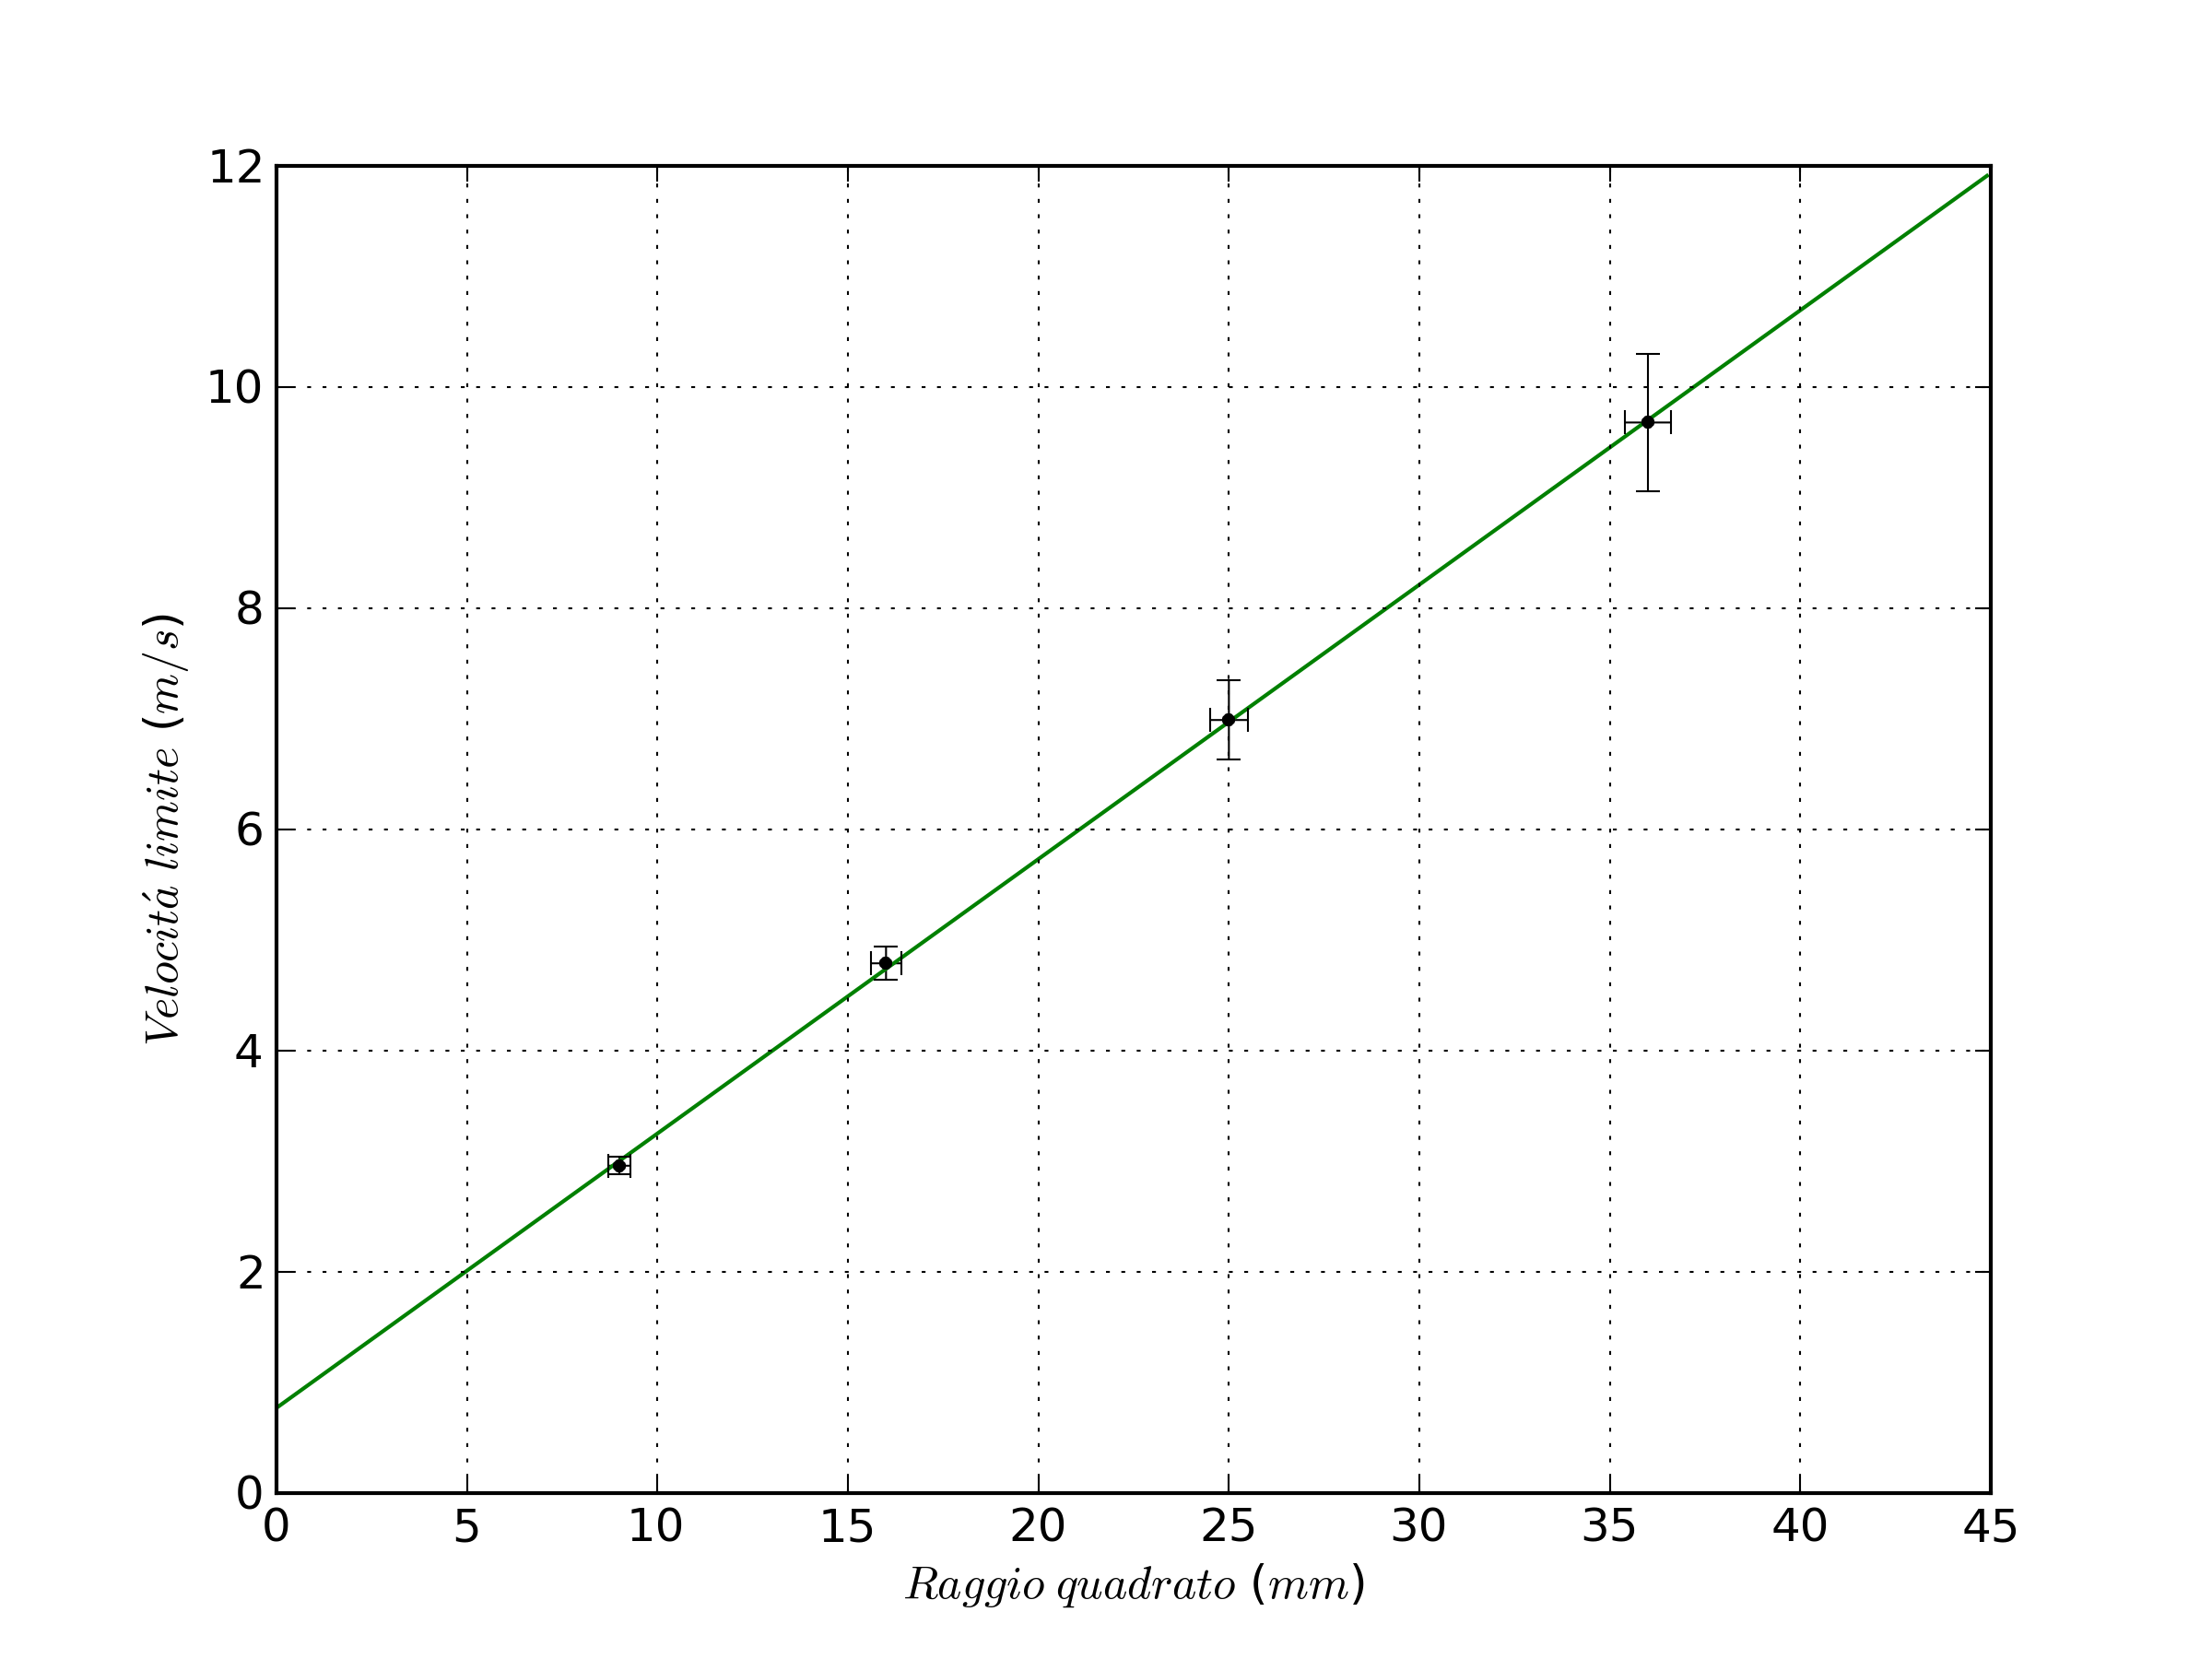
\includegraphics[scale=0.75]{../grafici/velocita}
\end{center}

Notiamo che il coefficente angolare $m$ dell'equazione \label{vlim} è dato da:
\begin{equation}
m= \frac{2g(\rho_{sfera} - \rho_{liquido})}{9 \eta}
\end{equation}

Conoscendo il valore numerico di $m$, possiamo ricavare il coefficente di viscosità.

\begin{equation}
\eta = \frac{2g(\rho_{sfera} - \rho_{liquido})}{9 m}
\end{equation}

$$\eta = $$

L'incertezza su 


\subsection*{Errore sistematico}
\section{Conclusioni}

%\chapter{Pendolo a torsione}
\section{Introduzione}
\subsection{Oggetto della ricerca}
L'esperienza si prefissa l'obiettivo di misura le costanti di torsione $c$ di tre fili di sezione differente e i momenti d'inerzia di tre oggetti.
\subsection{Metodo}
L'esperienza si compone di tre differenti fasi.
\begin{itemize}
\item Misura sperimentale dello spostamento angolare a seguito del momento della forza peso, al fine di calcolarne il momento d'inerzia 
\item Misura sperimentale del periodo di un pendolo di torsione, al fine di calcolare la costante di torsione dei fili
\item Misura della costante $c$ di torsione tramite l'instaurazione di un equilibrio tra il momento elastico e il momento della forza peso, e confronto con il valore teorico di $c$
\end{itemize}
\subsection{ Strumentazione e dati geometrici}
Nell'esperimento verrà utilizzato un pendolo di torsione strutturato nel seguente modo:
\\
Micrometro: $ \pm 1 \mu m$
 \\
Metro: $\pm 1 mm$
\\
Sensore di rotazione: $\pm 0.09$ gradi
\\

\begin{tabular}{ll}
Masse puntiformi: & 0.074 kg\\
Lunghezza sbarra: & 0.38 m\\
Massa Sbarra: & 0.2563 kg\\
Raggio Sbarra: & 0.0045 m\\
\midrule
Massa anello: & 0.46927 kg\\
Raggio interno: & 0.0265 m\\
Raggio esterno: & 0.0355 m\\
\midrule
Supporto & 0.0035 m\\
\midrule
Massa disco: & 0.12055 kg\\
Raggio disco: & 0.0475 m\\
Diametro carrucola: & 29 mm\\
\end{tabular}

\section{Raccolta dei dati}
Per quanto riguarda i tre fili in esame:
\begin{center}

\begin{tabular}{l|c|c|c|}
 & Filo A & Filo B & Filo C \\
\midrule
Diametro (mm) & 1.750 & 1.175 & 0.880 \\
Lunghezza (cm) & 41.3 &  43 & 33.5 \\
\midrule
\end{tabular}\end{center}

\subsection{Misura dei momenti d'inerzia}

In questa fase si provvederà a ricavare  sperimentalmente i momenti d'inerzia dei seguenti corpi:
\begin{itemize}
\item Disco 
\item Anello
\item Sbarra cilindrica omogenea, con due masse uguali, scorrevoli su di essa, poste equidistanti dall’asse di rotazione (a una distanza di $38\ cm$
\end{itemize}

Si è utilizzato un sistema di due pulleggie e un sensore di rotazione.
Il sensore di rotazione fornisce la posizione angolare in funzione del tempo. 
\\

Acquisiti i dati della posizione angolare in funzione del tempo, è possibile calcolare l'accelerazione angolare del sistema. A questo punto, si può calcolare $I$ nel seguente modo:
$$ bF_p = I\alpha $$
$$ I = \frac{b\cdot mg}{\alpha} $$

\begin{center}
\begin{tabular}{c|ccc}
Oggetto & Accelerazione angolare ($rad/s$) & Momento d'inerzia ($ 10^{-4} \cdot kg\cdot m^2$) \\
\midrule
Anello 60 g&43.05 & 1.983 \\
Anello 75 g &67.48 & 1.581 \\
Anello 100 g&84.43 & 1.685\\
\midrule
Media e $\sigma$&&1.750 $\pm$ 0.209 \\
\midrule
Disco e Anello 60 g&43.05 & 6.637 \\
Disco e Anello 75 g &67.48 & 6.639 \\
Disco e Anello 100 g&84.43 & 6.71\\
Disco e Anello 250 g&43.05 &  6.91 \\
\midrule
Media e $\sigma$&& 6.726 $\pm$ 0.1329\\
\midrule
Sbarra 60 g&43.05 & 50.12\\
Sbarra 100 g &67.48 & 55.78 \\
Sbarra 250 g&84.43 & 56.63\\
\midrule
Media e $\sigma$&& 54.18 $\pm$ 3.539\\
\midrule
\end{tabular}
\end{center}

Per quanto riguarda i momenti d'inerzia \textbf{teorici}:
$$ I_{sbarra} = \frac{1}{2} m R^2 = 84.4\cdot 10^{-4}\ kg\cdot m^2$$
$$ I_{anello} =\frac{1}{2} m (R^2_1 + R^2_2) = 1.3\cdot 10^{-4} \ kg\cdot m^2$$
$$ I_{disco} = \frac{1}{12} m L^2 + 2 \mu D^2 = 4.6\cdot 10^{-4} \ kg \cdot m^2$$



\subsection{Misura dinamica (pendolo di torsione)}

Abbiamo ricavato i seguenti periodi di oscillazione per ogni filo:
\\
\begin{tabular}{cc}
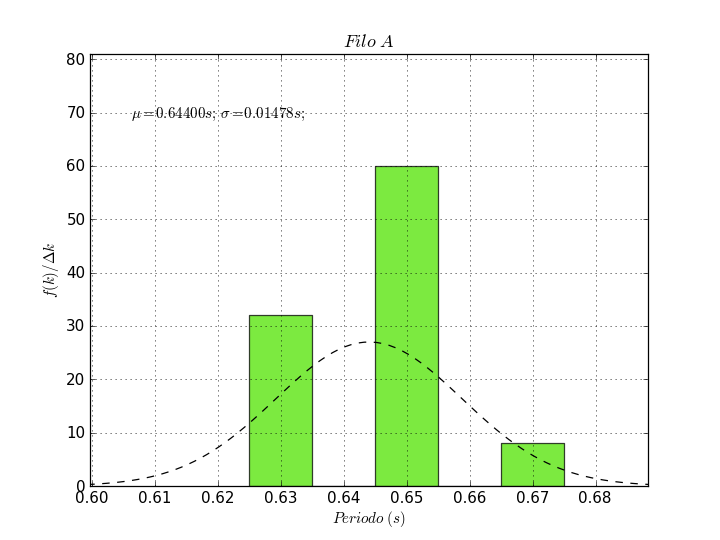
\includegraphics[scale=0.4]{../grafici/FiloA.png}
&
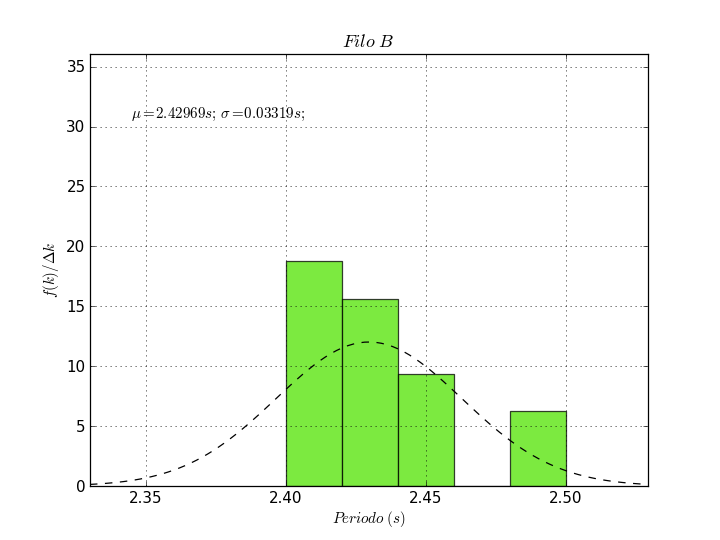
\includegraphics[scale=0.4]{../grafici/FiloB.png}
\\
\begin{tabular}{ll}
Filo A: & $0.644 \pm 0.015\ s$\\
Filo B: & $2.429 \pm 0.033\ s$\\
Filo C: & $3.844 \pm 0.046\ s$
\end{tabular}
&
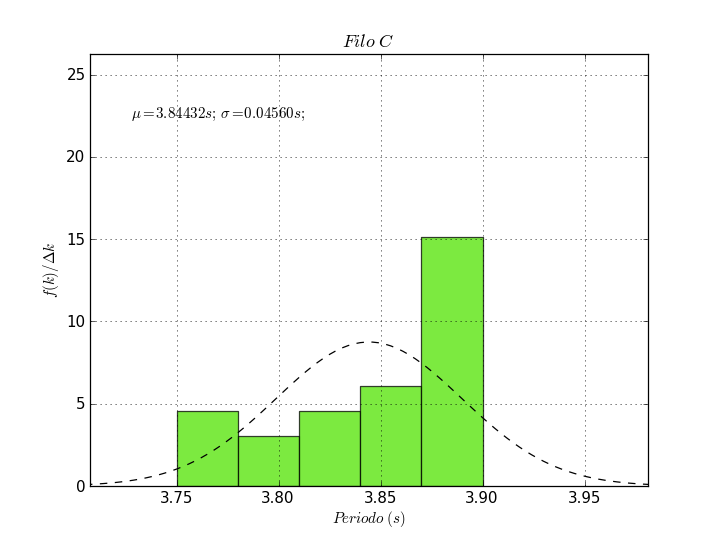
\includegraphics[scale=0.4]{../grafici/FiloC.png}\\

\end{tabular}


Questo ci permette di calcolare la costante di torsione $c$ sfruttando la seguente eguaglianza:
$$ -c\theta = I\frac{d^2\theta}{d\theta^2} $$
che identifica un moto oscillatorio di periodo
$$ T = 2\pi \sqrt{\frac{I}{c}}$$
da cui
$$ c = 4\pi^2\frac{I}{T^2} $$
Riassumendo:

\begin{center}
\begin{tabular}{l||c|c}
& Periodo ($s$) & Costante di torsione ($N\cdot m\cdot rad^{-1}$) \\
\midrule
Filo A: & $0.644 \pm 0.015$ & 95 \\
Filo B: & $2.429 \pm 0.033$ & 6.69\\
Filo C: & $3.844 \pm 0.046$ & 2.67\\
\end{tabular}
\end{center}


\subsection{Misura statica}

Tabulati gli angoli di deflessione per ogni filo in base alla massa sospesa (controlla!)\\
\begin{center}
\begin{tabular}{l|ccc}
& Filo A & Filo B & Filo C \\
\midrule
50g & 4.0 & 12.0 & 31.0 \\
100g & 7.0 & 23.0 & 61.0 \\
200g & 13.0 & 47.0 & 126.0 \\
\midrule
\end{tabular}\end{center}
Essendo il pendolo in equilibrio, poniamo
$$ \tau_{peso} = \tau_{elastico} $$
$$ b\cdot mg = c\theta $$
da cui
$$ c = \frac{b\cdot mg}{\theta} $$
dove $b$ è il braccio di applicazione della forza peso, ovvero il raggio della carrucola.
I valori di $c$ calcolati sono dunque stati (in $N\cdot m\cdot rad^{-1}$):

\begin{center}
\begin{tabular}{l|lll}
Peso & Filo A & Filo B & Filo C \\
\midrule
50g & 0.1019 & 0.0340 & 0.0135 \\
100g & 0.1164 & 0.0354 & 0.0134 \\
200g & 0.1254 & 0.0347 & 0.0129 \\
\midrule
$c_{best}$ & $0.115$ & $0.035$& $0.0137$ \\
$\sigma_{c}$ & $0.012$ & $\sim0$ & $\sim 0$ \\
\end{tabular}
\end{center}

\section{Dipendenza di $c$ da $r^4$}

Per la misura statica di $c$, bisogna utilizzare la seguente relazione:

$$ c = G \frac{\pi}{2}\frac{r^4}{l} $$

dove $G$ è il modulo di rigidità o di scorrimento ed è una proprietà specifica del materiale di cui il filo è realizzato.

Non siamo riusciti a trovare i valori di G tabulati in quanto non conoscevamo il materiale in cui era costruito il filo, quindi abbiamo cercato di arrivare a una migliore stima per riconoscerlo. Abbiamo utilizzato il valore di $c$ misurato in precedenza (misura statica) per calcolare $G$ secondo la seguente formula:

$$ G = \frac{2cl}{\pi r^4} $$

I valori calcolati sono stati:
\begin{center}
\begin{tabular}{lll}
Filo A & Filo B & Filo C \\
\midrule
49 GPa & 78 GPa & 73 GPa \\
\end{tabular}
\end{center}

Da cui abbiamo supposto che il filo A fosse in acciaio, e i fili B e C in titanio.
I dati ufficiali tabulati infatti sono i seguenti:
\begin{center}
\begin{tabular}{ll}
Acciaio & Titanio \\
\midrule
41 GPa & 78 GPa \\
\end{tabular}
\end{center}
Ripetendo il calcolo con G come tabulato, otteniamo:
\begin{center}
\begin{tabular}{lll}
Filo A & Filo B & Filo C \\
\midrule
0.0914 & 0.0339 & 0.0137 \\
\end{tabular}
\end{center}

che è compatibile con i valori misurati in precedenza.

\section{Conclusioni}
Confrontiamo i valori di $c$ teorici e calcolati tramite il metodo statico:
\begin{center}
\begin{tabular}{l|lll}
& Filo A & Filo B & Filo C \\
\midrule
Misura dinamica &  \\
Misura statica & $0.115\ (\pm 0.012)$ & $0.035$& $0.0137$ \\
Misura teorica & 0.0914 & 0.0339 & 0.0137 \\
\midrule
Misura media & 0.103 & 0.03445 & 0.0137\\
Errore ($\sigma_c$) & 0.017 & $\sim 0$ & $\sim 0$\\
\end{tabular}
\end{center}

Per tutti i fili la misurazione statica è ottima, tranne per il filo A, dove la misura è comunque confrontabile. A questo si aggiunge l'incertezza derivante dal non conoscere il materiale di costruzione dei fili.


\chapter{Oscillazioni smorzate e forzate}


\section{Introduzione}

Oggetto di questa ricerca è lo studio delle oscillazioni smorzate e forzate di un pendolo. Studiando il variare delle oscillazioni al variare della frequenza operativa della forzante, si studierà il fenomeno della risonanza.

\subsection{Strumenti}
\begin{center}
\begin{tabular}{l|l}
\midrule
Strumento & Precisione\\
\midrule
Calibro & $\pm 0.05$ mm\\ 
Sensore di rotazione & $\pm 0.00157$ rad\\ 
Alimentatore & $\pm 0.01$ V\\ 
\midrule 
\end{tabular}
\end{center}
L'attrezzatura utilizza è costituita da un disco metallico fissato ad una puleggia. La puleggia è messa in oscillazione da un filo alle cui estremità vi sono un oscillatore  elettromeccanico, che agisce come forzante, e un sistema di due molle. Al disco è possibile avvicinare e allontanare un magnete, che ha la funzione di smorzare il moto.

\subsection{Oscillazioni libere}

Si pone in oscillazione il disco, con il magnete  posizionato lontano e l'oscillatore elettromeccanico spento. Un sensore di posizione misura lo spostamento angolare; il sensore è collegato ad un computer, ed il programma DataStudio traccia in tempo reale il grafico dello spostamento angolare in funzione del tempo. Si interpolano dunque i dati con una funzione sinusoidale per determinare il periodo e la pulsazione delle oscillazioni e si ricava: $$T=1.47\pm0.02\ s \hspace{1cm} \omega=4.272\ rad/s$$ L'errore riportato è quello che il programma stesso attribuisce alla rilevazione, ed è determinato dalla precisione degli strumenti di rilevamento e dall'interpolazione dei dati.

\subsection{Oscillazioni smorzate}

Si avvicina il magnete al disco metallico. Il moto oscillatorio risulterà così smorzato per effetto delle correnti di Focault.
I dati raccolti dal sensore sono stati interpolati con la funzione
$$ \theta (t) = A_0 e^{- \gamma t} \sin(wt+\phi)+\theta_0 $$
al fine di determinare i parametri liberi; i valori ottenuti sono riportati di seguito in tabella.\\

$$T=1.45\ s$$

\begin{center}
\begin{tabular}{l|l|l}
\midrule
Parametri & Valore ricavato & $ \pm \sigma$ \\
\midrule
$A_0$ & 3.08 rad & 0.020\\
$\gamma$ & 0.197 $m^4/kg$& 0.0019\\
$\omega$ & -4.27 rad/s& 0.0019\\
$\phi$ & 1.93 rad & 0.0069 \\
$\theta_0$ & -1.53 rad& 0.0019 \\
\midrule
\end{tabular}
\end{center}

A questo punto, noti $\omega$ e $\gamma$, è possibile calcolare $ \omega_0 $, cioè la pulsazione per le oscillazioni libere, tramite l'equazione:
\begin{equation}\label{eq:omega}
\omega = \sqrt{\omega_0^2 - \gamma^2}
\end{equation} da cui:
$$\omega_0 = 4.275\ rad/s$$

Confrontandolo con il valore che avevamo ricavato interpolando direttamente il grafico delle oscillazioni libere si nota che i due non coincidono, ma che quello misurato dal periodo delle oscillazioni libere è minore di quello ricavato dalla formula: infatti, essendo un sistema reale, tra le sue parti sono presenti degli attriti che smorzano le oscillazioni.

\section{Oscillazioni smorzate-forzate}

Mantenendo il magnete vicino al disco, si mette in azione l'oscillatore elettromeccanico, che fornisce una componente forzante. Variando il voltaggio dell'alimentatore,  la frequenza di rotazione dell'oscillatore cambia: cerchiamo la frequenza di risonanza del sistema.
Poiché il periodo dell'oscillatore armonico coincide con quello della forzante (prima di raccogliere i dati si attende che il sistema si sia stabilizzato), possiamo leggere direttamente il periodo dal valore restituito dalla fotocellula.
Dopodiché abbiamo interpolato questi dati con il programma DataStudio, secondo la funzione
\begin{equation} \label{A}
A(\omega) = \frac{M_0}{\sqrt{ ({\omega_0}^2-\omega^2)^2 + 4\gamma^2\omega^2}}
\end{equation}

ed abbiamo ricavato così i valori corrispondenti ai parametri liberi $M_0$, $\gamma$ e $\omega_0$. 

Tale procedura è stata ripetuta spostando il magnete a distanze differenti dal disco.
\\
Di seguito sono riportati i dati raccolti e i rispettivi grafici. Di fianco alle tabelle si trovano i parametri ricavati dall'interpolazione con una sinusoidale, mentre sotto i grafici i valori ottenuti dall'interpolazione con la funzione \ref{A}. Tra la tabella e il grafico si trova invece il valore di $\omega_0$ ottenuto dalla \ref{eq:omega}.

\subsubsection{4.80mm}

\begin{center}
\begin{tabular}{c c}
\begin{tabular}{c | c | c}
\textbf{Ampiezza ($rad$)} & \textbf{Periodo ($s$)} & \textbf{Pulsazione ($rad/s$)}\\
\midrule
0.89 & 5.45 & 1.15\\
0.94 & 4.78 & 1.31\\
1.05 & 3.57 & 1.75\\
1.09 & 3.19 & 1.97\\
1.30 & 2.46 & 2.55\\
1.30 & 2.59 & 2.42\\
1.84 & 2.06 & 3.05\\
1.91 & 1.90 & 3.31\\
3.42 & 1.70 & 3.69\\
6.35 & 1.59 & 3.95\\
1.19 & 1.14 & 5.51\\
\end{tabular}

& 
\begin{tabular}{c}
$M_0=15.13\pm0.27$\\
\\
$\omega_0=4.25\pm0.01\ rad/s$\\
\end{tabular} 

\end{tabular}

\end{center}
 
\begin{center}

\includegraphics[scale=0.5]{"../grafici/Magnetea48mm"}

$$ \omega_0 = 4.25\ rad/s $$
$$ \gamma = 0.193\ s^{-1}$$
$$ M_0 = 15.3\ s$$


\end{center}
 
 
\subsubsection{2.80mm}

\begin{center}

\begin{tabular}{c c}

\begin{tabular}{c | c | c}
\textbf{Ampiezza} ($rad$) & \textbf{Periodo} ($s$) & \textbf{Pulsazione} ($rad/s$)\\
\midrule
1.68 & 2.00 & 3.14\\
2.95 & 1.63 & 3.85\\
3.22 & 1.44 & 4.36\\
2.17 & 1.30 & 4.83\\
1.20 & 1.15 & 5.46\\
1.67 & 1.24 & 5.06\\
0.99 & 1.10 & 5.71\\
0.68 & 0.98 & 6.40\\
0.51 & 0.89 & 7.06\\
0.26 & 0.74 & 8.49\\
\end{tabular}

& \hspace{1cm}

\begin{tabular}{c}
$A_0 = 3.4 \pm 0.020\ rad$\\
\\
$\gamma =  0.636 \pm 0.0057\ m^4/kg $\\
\\
$\omega = -4.25  \pm 0.0064\ rad/s $\\
\\
$\phi =  2.38 \pm 0.0076\ rad $ \\
\\
$\theta_0 = -0.57 \pm 0.0038\ rad $\\

\end{tabular}

\end{tabular}

\end{center}

$$\omega_{0} = 4.297\ rad/s$$
\begin{center}
\includegraphics[scale=0.5]{"../grafici/Magnetea28mm"}

$$ \omega_0 = 4.26\ rad/s $$
$$ \gamma = 0.543\ s^{-1} $$
$$ M_0 = 15.6\ s$$

\end{center}


\subsubsection{1.00mm}

\begin{center}

\begin{tabular}{c c}

\begin{tabular}{c | c | c}

\textbf{Ampiezza} ($rad$) & \textbf{Periodo} ($s$) & \textbf{Pulsazione} ($rad/s$)\\
\midrule
1.33 & 2.01 & 3.12\\
1.42 & 1.85 & 3.39\\
1.45 & 1.67 & 3.76\\
1.18 & 1.31 & 4.79\\
1.31 & 1.39 & 4.52\\
1.47 & 1.54 & 4.07\\
0.76 & 1.09 & 5.76\\
0.88 & 1.19 & 5.28\\
1.01 & 1.22 & 5.15\\
0.49 & 0.93 & 6.75\\
0.65 & 1.03 & 6.10\\
0.39 & 0.85 & 7.39\\

\end{tabular}

& \hspace{1cm}

\begin{tabular}{l}

$A_0 = 18600 \pm 1300\ rad$ \\
\\
$\gamma= 1.50 \pm 0.0011\ m^4/kg$\\
\\
$\omega = 4.02 \pm 0.0077\ rad/s$\\
\\
$\phi =  26.3 \pm 0.0046 \ rad/s$ \\
\\
$\theta_0 = 0.055 \pm 0.0016\ rad$ \\

\end{tabular}

\end{tabular}

\end{center}


$$\omega_{0} = 4.291\ rad/s $$

\includegraphics[scale=0.75]{"../grafici/Magnetea10mm"}


$$ \omega_0 = 4.37\ rad/s $$
$$ \gamma = 1.40 \pm 0.14\ s^{-1}$$
$$ M_0 = 17.1 \pm 1.4\ s$$


\section{Risonanza}
\section{Conclusioni}
L'esperimento è riuscito un sacco.

\section{Fenomeno}
Sovvrapponendo le curve trovate in precedenza, possiamo apprezzare un grafico nel quale si mette in evidenza la risonanza. 
Verifichiamo anche la condizione di risonanza Con l'approssimarsi di $\gamma $ a zero, il valore dell'ampiezza tende a $\infty$.




























































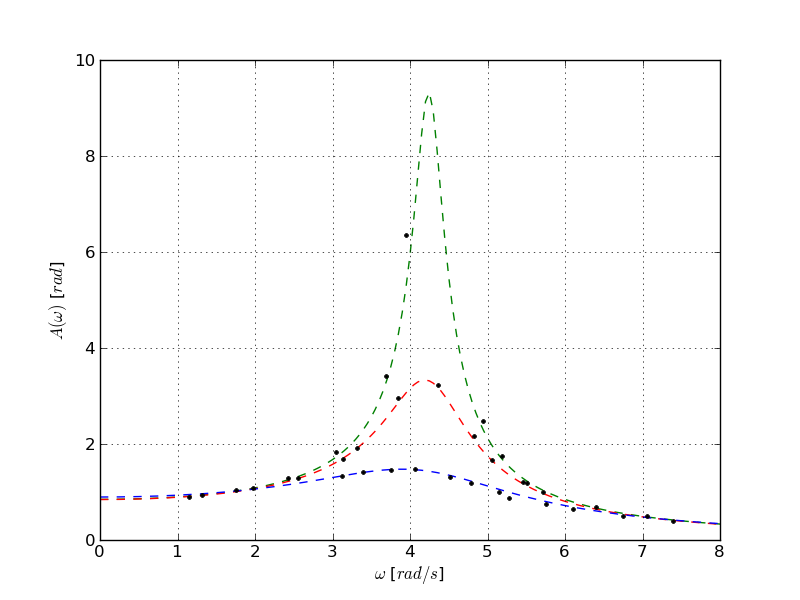
\includegraphics[scale=0.9]{../grafici/risonanza}

%\chapter{Bilancia di Cavendish}
\section{Introduzione}
\subsection{Oggetto della ricerca}
Misurazione della costante di gravitazione G mediante la bilancia di Cavendish.
\subsection{Proprietà geometriche dei corpi e strumentazione}

\begin{tabular}{ll}
m=38.3$\pm$0.2 g & massa sfere piccole\\
M=1500$\pm$10 g	 & massa sfere grandi\\
r=9.53 mm & raggio sfere piccole\\
R=31.9 mm & raggio sfere grandi\\
L=5.50m & distanza schermo-bilancia \\
$m_c\cong 2m$ & massa manubrio\\
b = 46.5 mm &\\
d = 50 mm &\\
\end{tabular}


\begin{center}
 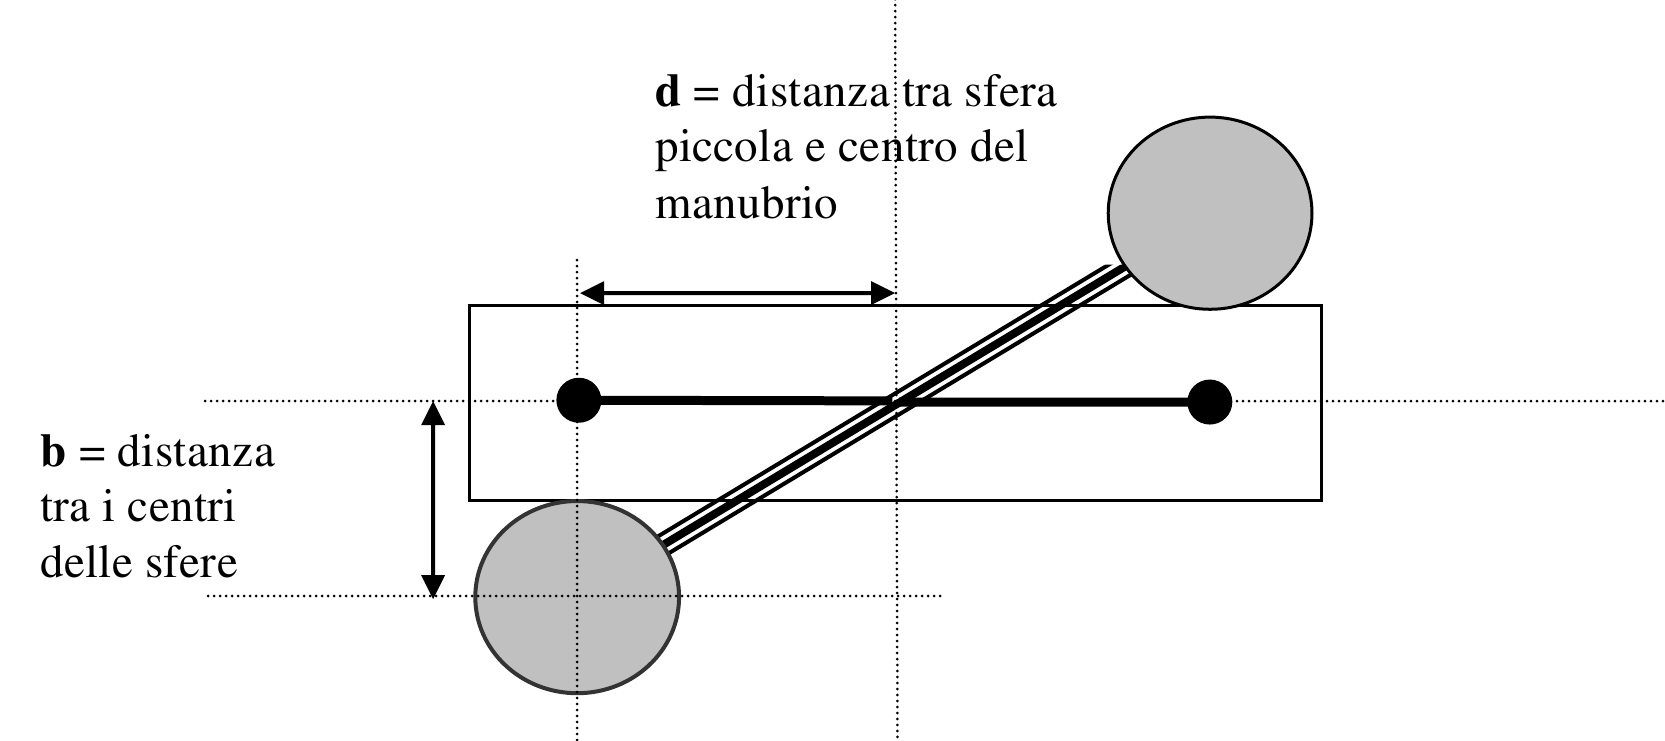
\includegraphics[scale=0.25]{../grafici/cavendish/schema.png}
\end{center}

Il momento d'inerzia $I$ del corpo si calcola:

$$ I=2m(d^2+2/5r^2) = 1.94283 \cdot 10^{-4} kg\cdot m^2$$
L'incertezza sul momento di inerzia è dell'ordine di $10^{-6}$, ed è perciò trascurabile. 
\subsection{Metodo in breve}
La bilancia di Cavendish è uno strumento estemamente sensibile utilizzato per misurare forze di bassissima entità. Il principio su cui si basa è quello dell'equilibrio tra due momenti torcenti: quello della forza di gravità e quello dovuto alla torsione del filo. Questo equilibrio non si raggiunge istantaneamente, ma è necessario attendere un certo tempo, entro il quale il pendolo oscillerà (in modo smorzato).

Per trovare la posizione di equilibrio basterà ricercare una media (mobile) tra i le posizioni di massimo e di minimo.

\begin{center}
 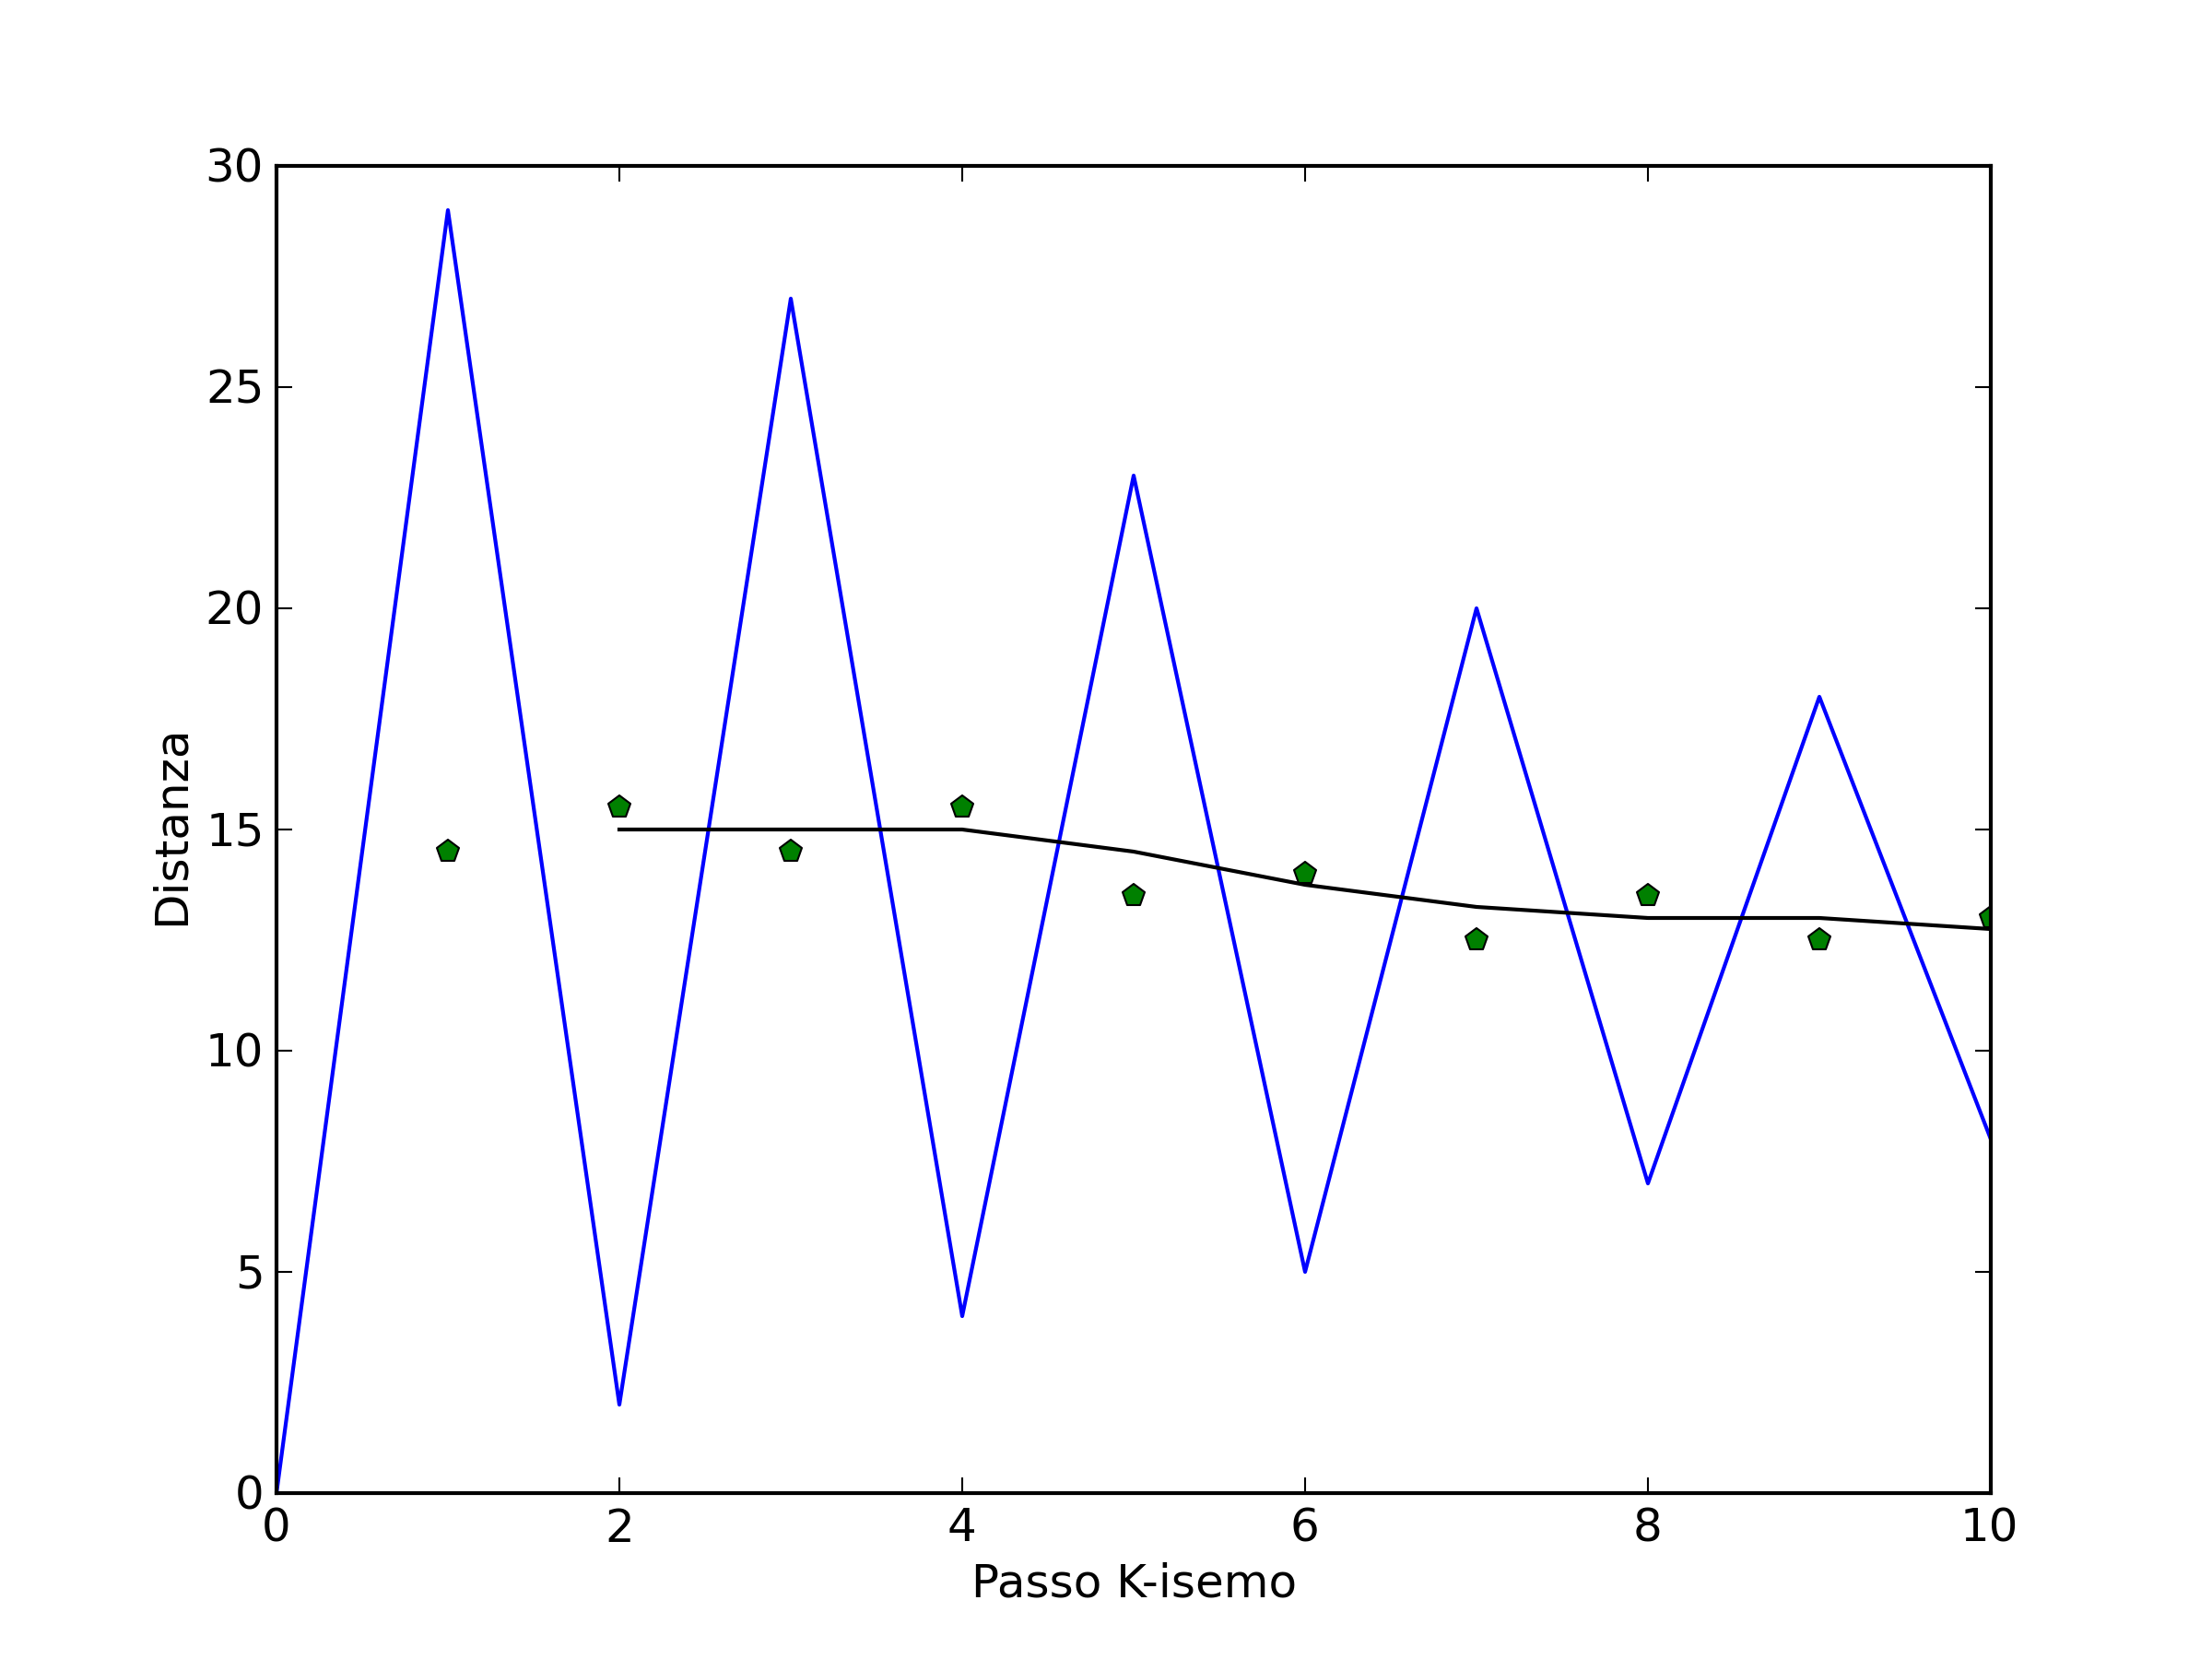
\includegraphics[scale=0.50]{../grafici/cavendish/oscillazioni.png}
\end{center}

Essendo le oscillazioni del pendolo molto piccole, queste vengono amplificate grazie a un laser, che viene fatto incidere sul pendolo, e viene riflesso su di una parete distante circa 5.50 m.

La misurazione sulla posizione di equilibrio e in generale sulla posizione del pendolo vengono effettuate su di un nastro di carta graduata attaccata alla parete.


\section[Misura di k e theta]{Misura $k$ e $\theta$}
L'incertezza relativa allo strumento per la misurazione del periodo è trascurabile rispetto l'entità della misura. Non è così per quella da attribuire allo sperimentatore, che è infatti molto elevata.

Il periodo misurato è dunque ottenuto come media di 5 periodi. L'incertezza è la massima stimata e dipende interamente dallo sperimentatore.

$$T = 513 \pm 20 \ s$$

Per ricavare $k$, ricordiamo che:
$$T^2 = 4 \pi^2 \frac{I}{k}$$
Quindi
$$k = 4 \pi^2 \frac{I}{T^2} = 2.84 \cdot 10^{-8}\ kg\cdot m^2\cdot{s}^{-2}$$
Per quanto riguarda $\theta$, chiamando $s_1$ la prima posizione di equilibrio e $s_2$ la seconda, si ha che:
$$ tan(4\theta) = \frac{s_1-s_2}{L} $$
dove $s_1-s_2$ vale 0.115 m. Si misura $4\theta$ perché la rotazione di $\pi/2$ delle masse più grandi fornisce una rotazione della bilancia pari a $2\theta$ rispetto alla posizione di equilibrio, che va raddoppiata, misurando noi l'angolo riflesso.
$$ \theta = \frac{arctan(\frac{s_1-s_2}{L})}{4} \simeq 5.23 \cdot 10^{-3} rad $$
Inoltre, chiamamdo $F_G$ la forza di attrazione tra una sferetta piccola e quella grande più vicina, si ha che:
$$ \tau_G = 2dF_G = G\frac{mM}{b^2}2d $$
ma per ipotesi
$$ \tau_T = -k\theta = -\tau_G $$
$$ G\cdot\frac{2mMd}{b^2} = k\theta $$
dunque:
$$G = \frac{k \theta b^2}{2mMd} = 5.733 \cdot 10^{-11}\ {m}^3\cdot {kg}^{-1}\cdot{s}^{-2}$$

\section{Analisi dati} 

Correzione:
Bisogna applicare una correzione a $G$, dovuta dall'attrazione che non è stata considerata, tra le sferette piccole e le masse più lontane, che tende a fare ruotare il pendolo in senso opposto. Infatti, questa forza ($F_{G_2}$) fornsce un contributo negativo, e dunque noi con l'esperimento in realtà abbiamo misurato una forza data da:

\begin{equation}\label{eq:fgrav}
 F_{G'} = F_G - F_{G_2}
\end{equation}

(nota: per chiarezza abbiamo preferito $G_t$ come abbreviazione il valore vero (corretto) di $G$, per non confonderla con $G'=G$ che abbiamo misurato prima)
Dunque, non abbiamo misurato il valore vero di $G$, ma un'altro valore, $G'$. Valendo però la relazione \ref{eq:fgrav}, $G_t$ e $G'$ sono legati da una relazione:

\begin{eqnarray*}
G'\cdot\frac{mM}{b^2} & = & G_tmM(\frac{1}{b^2} - \frac{1}{b^2+4d^2}) \\
                      & = & G_t\frac{mM}{b^2}(1 - \frac{b^2}{b^2+4d^2}) \\
\end{eqnarray*}

e quindi:
$$ \frac{G'}{G_t} = 1-\frac{b^2}{b^2+4d^2} = 0.822$$
sicché
$$ G_t = \frac{G'}{0.822}$$
Inoltre:

$$ G_t = 1.216\cdot \frac{\theta k b^2}{2mMd} = 6.9723\cdot 10^{-11}\ {m}^3\cdot {kg}^{-1}\cdot{s}^{-2}$$

%
\chapter{Banco Ottico}
\section{Introduzione}
\subsection{Scopo dell'esperimento e metodo in breve}

L'esperimento si compone di tre parti. Nella prima, si verifica la validità della Legge di Snell e la reversibilità del cammino ottico: dato un raggio luminoso attraversante un semi-cilindro in plexiglass, misuriamo l'angolo di incidenza $\theta_{rifrazione}$ ed il corrispondente  angolo di rifrazione $\theta_{rifrazione}$. Sempre grazie alla legge di Snell si ricerca la miglior stima dell'indice di rifrazione del plexiglass $n$.
\\


Nella seconda parte, si ricerca $n$ studiando l'angolo di deviazione minima $\delta_{min}$ di un prisma a base triangolare e di un prisma a base trapezoidale. Inoltre, si ricerca la distanza di cui viene traslato il raggio, che arriva con un certo angolo di incidenza $\theta$, quando passa per due superfici parallele.
\\

Infine si verifica la legge dei punti coniugati tramite la misura delle distanze $p$ e $q$ e la validità dell'ingrandimento ottico $M$. 

\subsection{Strumenti}
In questa tabella vengono riassunti gli strumenti rivelatori utilizzati, con le relative precisioni, e il set-up dell'esperimento.
\begin{center}
\begin{tabular}{c|c}
Strumento & Precisione \\
\midrule
Piatt. Graduata & $\pm 1 grado $ \\
Metro & $\pm 1 mm $\\
\end{tabular}
\end{center}

Per le prime due parti dell' esperimento, il proiettore è stato impostato sulla modalità a singolo raggio luminoso e successivamente sulla modalità oggetto per la terza e ultima parte. 
Il proiettore, insieme alla piattaforma girevole graduata, alle lenti ed a uno schermo bianco, può scorrere liberamente lungo una rotaia, permettendo di modificare le distanze tra gli oggetti a piacimento.

\section{Reversibilità del cammino luminoso}

Tutte le misure seguenti sono espresse in gradi.


\begin{table}
\center
\begin{tabular}{c|c||c|c}
 \multicolumn{2}{c}{\textit{Faccia piana}} &
\multicolumn{2}{c}{\textit{Faccia curva}} \\
$\theta_{incidenza} $ & $\theta_{rifrazione} $ &$\theta_{incidenza} $ & $\theta_{rifrazione} $\\
\midrule
 10 & 7 & 7 & 10 \\
15 & 10 & &\\
20 & \textbf{13.5} & 13.5 & 20\\ 
25 & \textbf{16.5} & & \\
30 & 20 & 30 & 20\\
40 & 26 & 26 & 40\\
35 & 23 & &\\
45&  \textbf{28.5} & & \\
\end{tabular}
\caption*{Misure in gradi}
\end{table}


Raccolti i valori degli angoli di incidenza e dei corrispondenti angoli di rifrazione, possiamo calcolare la miglior stima di $n$.
La legge di Snell esprime la relazione che lega gli indici di rifrazione dei due materiali attraversati dal raggio luminoso, e i seni degli angoli di incidenza e rifrazione:

\begin{center}
$n_1 sin\theta_1 = n_2 sin\theta_2$
\end{center}

Poiché $n_a \simeq1 $ ( indice di rifrazione dell'aria ), si ricava:

$$n_2 = \frac{sin\theta_1}{sin\theta_2}$$

Nell'elaborazione dei dati, abbiamo selezionato solo le coppie di misure cui corrispondesse un errore relativo percentuale minore del 6\%, al fine di avere una stima più precisa del valore vero di $n$.

\begin{center}
\begin{tabular}{c|c|c|c|c|c}
\textbf{$\theta_1$} & 25 & 30 & 40 & 35 & 45\\
\midrule
\textbf{$\theta_2$} & 16.5 & 20 & 26 & 23 & 28.5\\
\midrule
\textbf{$n_i$} (*) & 1.489 & 1.462 & 1.468 & 1.468 & 1.482\\
\end{tabular}\\

\end{center}

(*) in questo caso abbiamo tenuto un numero superiore di cifre significative, in quanto si tratta di calcoli intermedi 
%Ripensare alle cifre significative

$$\overline{n} = \frac{\displaystyle\sum\limits_{i=1}^N n_i}{N} = 1.474 $$

$$\sigma_n = \sqrt{\frac{\sum_{i=1}^N n_i}{N-1}} = 0.01$$

$$\sigma_{\overline{n}} = \frac{\sigma_n}{\sqrt{N}} = 0.004$$

$$n_{best} = 1.474  \pm 0.004 $$

%Cifre significative incertezza diverse da cifre significative misura!

\section{Misura dell'angolo di deviazione minima}


L'angolo di deviazione minima ($\delta_{min}$) è il più piccolo angolo misurato facendo incidere un fascio di luce sulla faccia di un prisma (con inclinazione variabile) e misurando l'ampiezza dell'angolo rifratto. Nel nostro esperimento abbiamo utilizzato due prismi: uno con base un triangolo equilatero e l'altro un trapezio rettangolo.
\\

In tabella sono riportati i valori trovati per ogni misurazione dell'angolo rifratto. Per aumentare il livello di precisione, abbiamo raccolto i dati relativi agli angoli di deviazione minima per ogni faccia di prisma a base triangolare, identificando ogni misurazione con il numero dello spigolo compreso tra le facce colpite e il verso di percorrenza della luce.
\\

Per ovvie ragioni geometriche, nel caso del prisma a base trapezoidale (è presente un solo angolo acuto, di 45 gradi) è stato impossibile effettuare misure riferite a vari vertici.

\begin{center}
\begin{tabular}{|c | c | c|}
\hline
Spigolo & $\delta_{min}$ (andata) & $\delta_{min}$ (ritorno)\\
\hline
\multicolumn{3}{|c|}{\textit{Prisma a base triangolare}} \\
\hline
1 & 41 & 31\\
2 & 43 & 39\\
3 & 41 & 41\\
\hline
\multicolumn{3}{|c|}{\textit{Prisma a base trapezoidale}} \\
\hline
1 & 28 & 21\\
\hline
\end{tabular}
\end{center}

$$\overline{\delta}_{min} = \frac{\displaystyle\sum\limits_{i=1}^6 \delta_i}{6} = 1.52$$

%Angolo deviazione minima, immagine
\subsection{Analisi dei dati}

\section{Lenti sottili}
\
Nell'ultima parte dell'esperimento, si verifica la validità della legge dei punti coniugati,
$$ \frac{1}{f} = \frac{1}{q} + \frac{1}{p} $$
\textit{p: distanza sorgente-lente}
\textit{q: distanza lente-schermo}
\textit{d: diametro circonferenza proiettata}

In tabella sono riportati sulla destra le misure effettuate con lente di focale $f=100 mm$, a sinistra con lente di focale $f=200mm$. Tutti i valori sono in cm.

\begin{center}
\begin{tabular}{*{3}{c|}*{3}{|c}}
p & q &d &p &q&d\\
\midrule
13.5 & 36.5 & 5.5 & 73.4 & 26.6 & 0.7\\
36.2 & 13.8 & 0.8 & 26.4 & 73.6 & 5.5\\
\midrule
18.0 & 22.0 & 2.5 & 61.5 & 28.5 & 0.9\\
22.0 & 18.0 & 2.1 & 28.1 & 61.9 & 4.8\\
\end{tabular}
\end{center}

Per verificare la validità, rappresentare su un grafico i punti ($\frac{1}{p};\frac{1}{q})$ e verificare che i punti sono disposti lungo una retta. 
\\
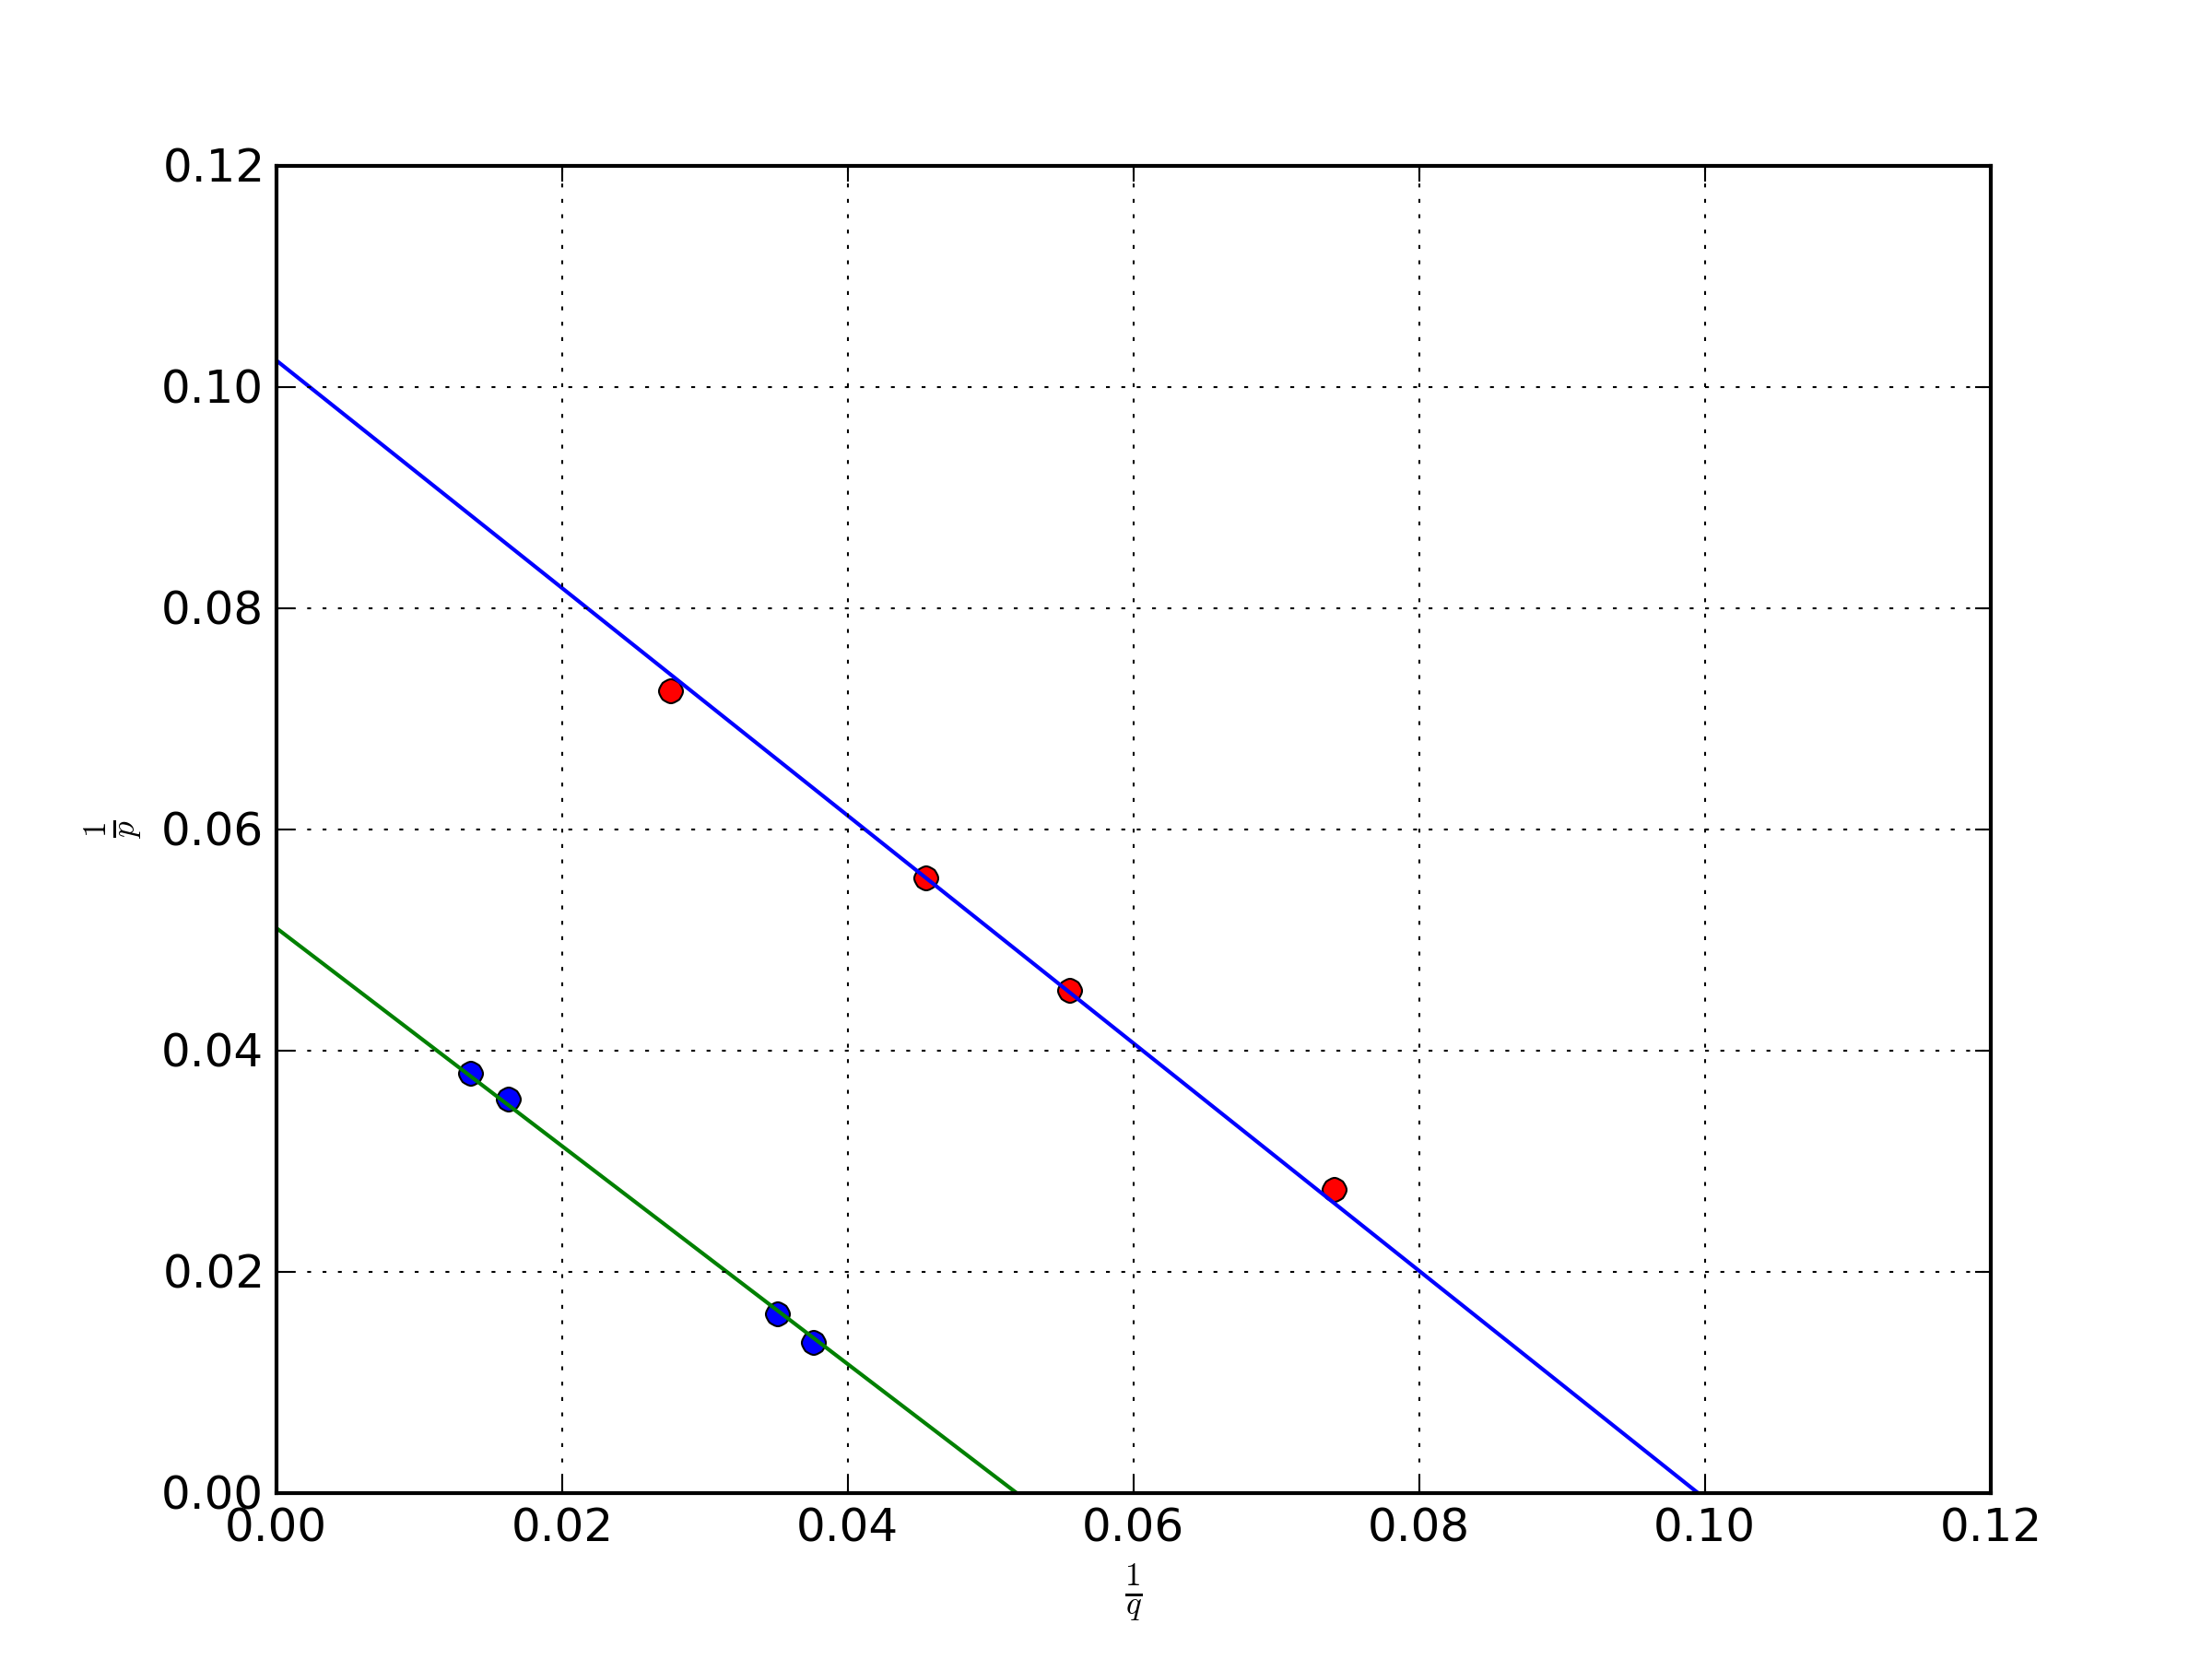
\includegraphics[scale=0.75]{../grafici/ottica}

L'intecetta trovata è $q_1 = 0.1024$ e $q_2 = 0.05108$.
Ricaviamo i valore della focale $f = \frac{1}{q}$. $f_{1} = 9.76\  cm$ e $f_{2} = 19.57\ cm$. 

L'incertezza sulla focale è data dall'espressione:
$$\delta f = \sqrt{\frac{q^4(\delta p)^2 + p^4(\delta q)^2}{(p+q)^2}}$$

ottenuta tramite il metodo delle derivate parziali.

$$\delta f_{1} = \pm 2.66\ cm $$ 
$$ \delta f_{2} = \pm 5.43\ cm $$




\chapter{Pendolo di Kater e caduta libera}
\section{Introduzione}

L'obiettivo dell'esperimento è misurare l'accelerazione gravitazionale $g$ attraverso due dei possibili metodi e confrontarli. 

\section{Pendolo di Kater}
\subsubsection{Introduzione}

Il pendolo di Kater è un pendolo fisico che può essere messo in oscillazione su due punti $c_1,\ c_2$ non coincidenti con il suo baricentro $G$. Il pendolo è costituito da un'asta rigida, due masse $m_a = 1400g$, $m_b=1000g$, di cui una mobile, e due coltelli, posizionati nei punti $c_1$ e $c_2$. La massa $m_a$ è mobile, e viene posizionata a varie distanze (misurate rispetto a $c_1$). Dopodiche!! vengono misurati e riportati in tabella i periodi di oscillazione del pendolo, facendolo oscillare prima su $c_1$ e poi su $c_2$.

Il periodo del pendolo dipende ovviamente dalla posizione del baricentro rispetto al punto di sospensione. Chiamando $h_i$ la distanza del punto $i\in\{1,2\}$ dal baricentro:

$$ T_i = 2 \pi \sqrt{\frac{L_i}{g}} = 2 \pi \sqrt{\frac{I_i}{m gh_i}}$$

dove $L_i$ e!! la lunghezza ridotta del pendolo, $m$ e!! la massa totale e $I_i$ il momento d'inerzia del pendolo appeso per il punto $i$-esimo.
\\
Se si individuano i due punti nel quale il periodo $T_1 = T_2$ allora l'equazione si riduce a:

$$ T = \ 2 \pi \sqrt{\frac{D}{g}}$$

La distanza $D= h_1 + h_2 $  è nota con grande precisione, e nel nostro caso e!! $D=99.4\ cm$. Misurando quindi il periodo $T$, possiamo calcolare $g$.
$$ g = \frac{4\pi^2D}{T^2}$$
\subsection{Procedimento}

In questo esperimento abbiamo utilizzato i seguenti strumenti:
\begin{itemize}
  \item Un metro a nastro, con sensibilita!! $1\ mm$
  \item Un cronometro digitale con fotocellula, che ha una precisione di $\pm 0.1 \cdot 10^{-3}\ s$
\end{itemize}

A questo punto abbiamo posto in oscillazione il pendolo dal coltello $c_1$ e si misura $T_1$, e abbiamo ripetuto l'operazione per il coltello $c_2$, misurando $T_2$, ripetendo la misura 10 volte per poter stimare l'errore sperimentale. (possible repetiscion)

Mantenendo fissa la massa $m_b$ ad una distanza $d = 15.4cm$ da $c_1$, allontaniamo o avviciniamo la massa $m_b$, e ripetiamo le misure.

La massa $m_a$ viene spostata per cercare una posizione in cui $T_1 \simeq T_2$, ovvero si e!! in una condizione per la quale $L\simeq h_1+h_2$. 

\subsection{Dati}
Nella tabella sono raccolti tutti i periodi $T_1,T_2$ misurati in secondi. $d$ è la distanza tra il coltello $c1$ e la massa $m_a$.
\begin{center}
\begin{tabular}{*{8}{c}}
$d$& $6.9\ cm$ & $11.7\ cm$ & $13.5\ cm$  & $15.0\ cm$ & $17.9\ cm$ & $85.0\ cm$ & $81.9\ cm$ \\
\midrule
 \textbf{Coltello 1}&& & & & & \\
&2.1197 &2.0040&2.0279 &1.9809 & 1.9211 & 1.9934 & 1.9735\\
 &2.1125&2.0041 &2.0029&1.9796 & 1.9207 & 1.9932 & 1.9744 \\
 &2.1179&2.0043 &2.0021&1.9816 & 1.9264 & 1.9931 & 1.9746 \\
 &2.1204&2.0062 &2.0042&1.9794 & 1.9253 & 1.9932 & 1.9755 \\
 &2.1189&2.0060 &2.0026&1.9821 & 1.9113 & 1.9932 & 1.9765 \\
 &2.1129&2.0052&2.0012&1.9805 & 1.9278 & 1.9934 & 1.9769 \\
&2.1125 &2.0050&2.0014&1.9802 & 1.9278 & 1.9937 & 1.9770 \\
&2.1131 &2.0061&2.0008&1.9804 & 1.9277 & 1.9941 & 1.9760 \\
 &2.1143&2.0046&2.0036&1.9810 & 1.9278 & 1.9937 & 1.9754 \\
 &2.1131&2.0058&2.0005& 1.9831 & 1.9278 & 1.9935 & 1.9750 \\
 \midrule
$\bar{x}$& 2.1158 & 2.0085 & 2.0021 & 1.9806 & 1.9244 & 1.9935 & 1.9755\\
$\sigma$ & 0.0032 & 0.0019 & 0.0012 & 0.0102 & 0.0053 & 0.0003 & 0.0011\\
\midrule
\textbf{Coltello 2} && & & & & \\
&2.0279&2.0041&1.9983 &1.9934 & 1.9882 & 1.9946 &	1.9802 \\
&2.0284&2.0043&1.9983 &1.9946 & 1.9902 & 1.9939 &	1.9812 \\
&2.0289&2.0062&1.9967 &1.9911 & 1.9907 & 1.9943 &	1.9820 \\
&2.0289&2.0060&1.9978 &1.9919 & 1.9908 & 1.9941 &	1.9818 \\
&2.0288&2.0052&1.9978 &1.9940 & 1.9907 & 1.9940 &	1.9819 \\
&2.0288&2.0050&1.9986 &1.9923 & 1.9907 & 1.9952 &	1.9813 \\
&2.0288&2.0061&1.9986 &1.9939 & 1.9888 & 1.9954 &	1.9816 \\
&2.0288&2.0046&1.9988 &1.9934 & 1.9898 & 1.9943 & 1.9818 \\
&2.0286&2.0058&2.0001 &1.9914 & 1.9898 & 1.9947 & 1.9812  \\
&2.0286&2.0040&1.9994 &1.9958 & 1.9878 & 1.9941 & 1.9810 \\
 \midrule
$\bar{x}$& 2.0827 & 2.0053 & 1.9984 & 1.9932 & 1.9832 & 1.9945 & 1.9814\\
$\sigma$ & 0.0003 & 0.0009 & 0.0009 & 0.0015 & 0.0017 & 0.0005 & 0.0005\\
\bottomrule
\end{tabular}
\end{center}

\subsection{Analisi}
Per semplicita!!, abbiamo deciso di concentrarci specialmente sul primo punto di intersezione tra le due curve, ottenuto inserendo in un grafico.


\begin{center}
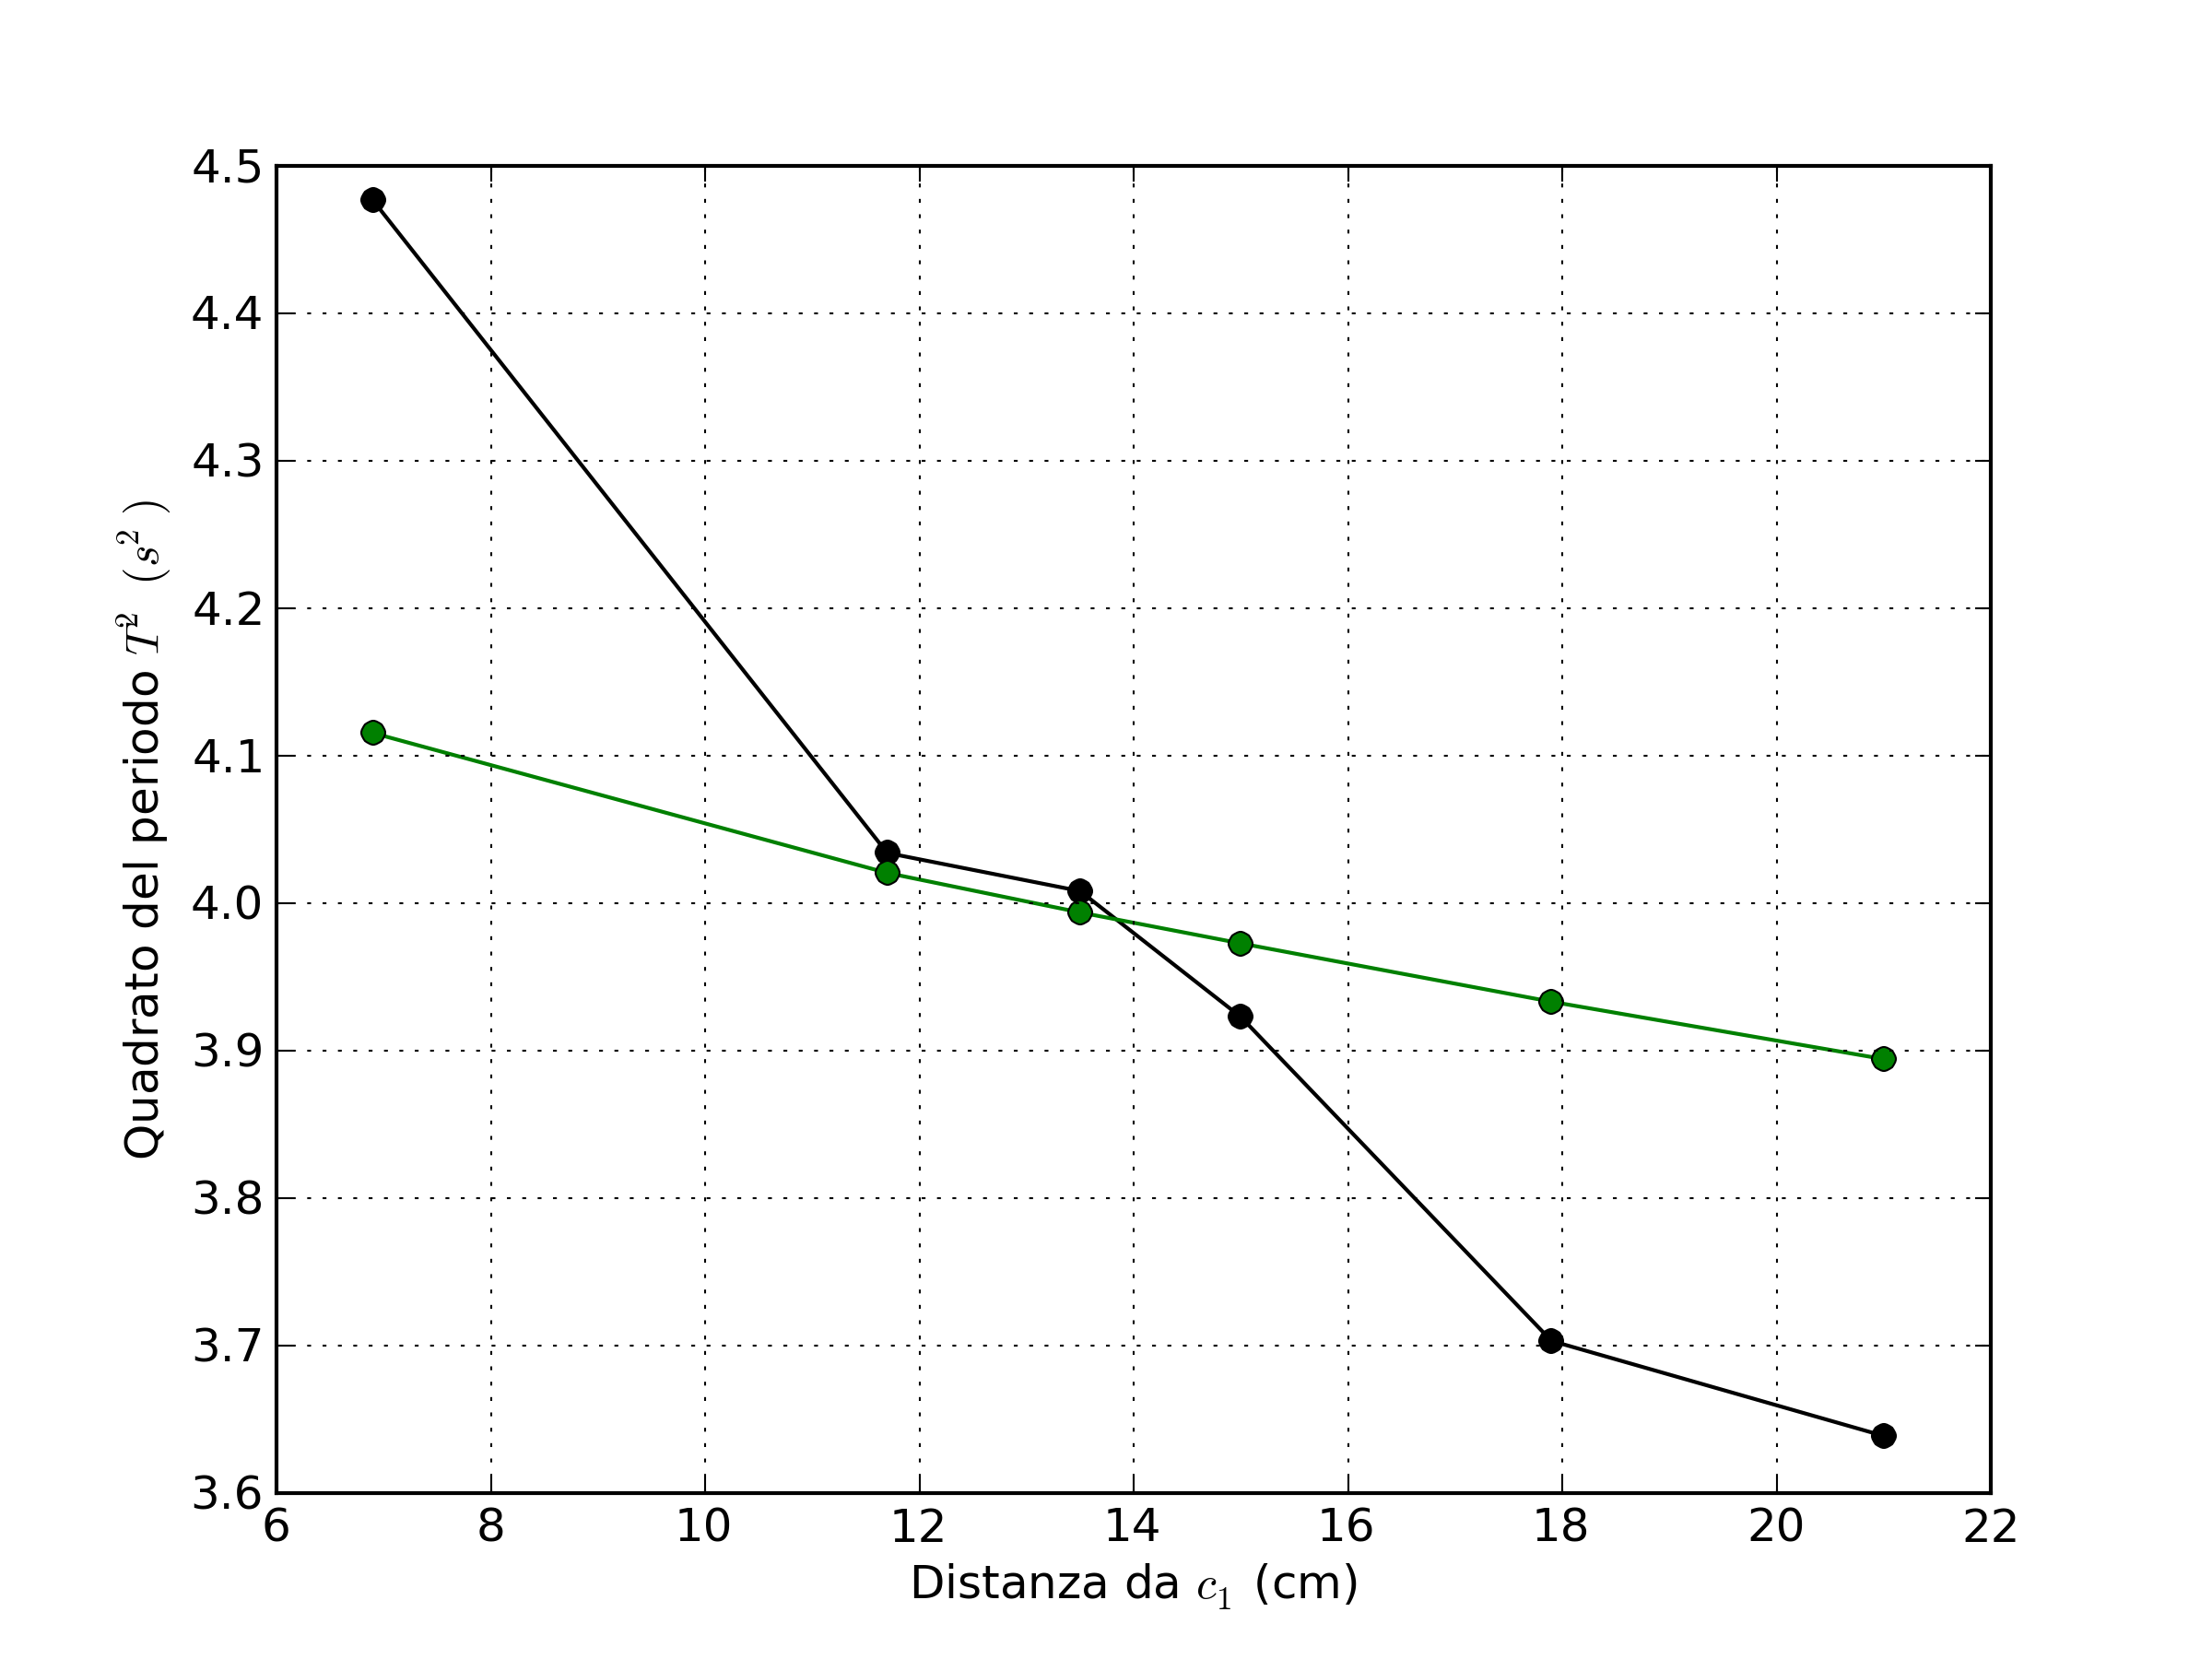
\includegraphics[scale=0.60]{../grafici/kater/kater-punti-raw.png}
\end{center}


\section{Caduta libera}


\subsection{Raccolta dati}
Tutti i valori riportati in tabella sono in millisecondi.
\begin{center}
\begin{tabular}{r|*{14}{c}}
\textbf{20 cm} & 197 & 199 & 197 & 200 & 199 & 203 & 200 & 203 & 196 & 199 & 196 & 199 & 197 & 205\\
& 198 & 199 & 198 & 197 & 199 & 198 & 197 & 198 & 200 & 198 & 199 & 199 & 198 & 204\\
\midrule
\textbf{35 cm} & 265 & 265 & 265 & 261 & 262 & 263 & 266 & 262 & 269 & 266 & 261 & 263 & 262 & 261\\
\midrule
\textbf{50 cm} & 314 & 315 & 314 & 321 & 319 & 316 & 315 & 315 & 315 & 314 & 314 & 315\\
\midrule
\textbf{60 cm} & 347 & 345 & 346 & 347 & 344 & 344 & 348 & 345 & 346 & 344 & 345 & 345\\
\midrule
\textbf{90 cm} & 424& 424& 424& 423& 425& 424& 426& 423& 424& 423& 422& 425& 423\\
\end{tabular}
\end{center}

\begin{center}
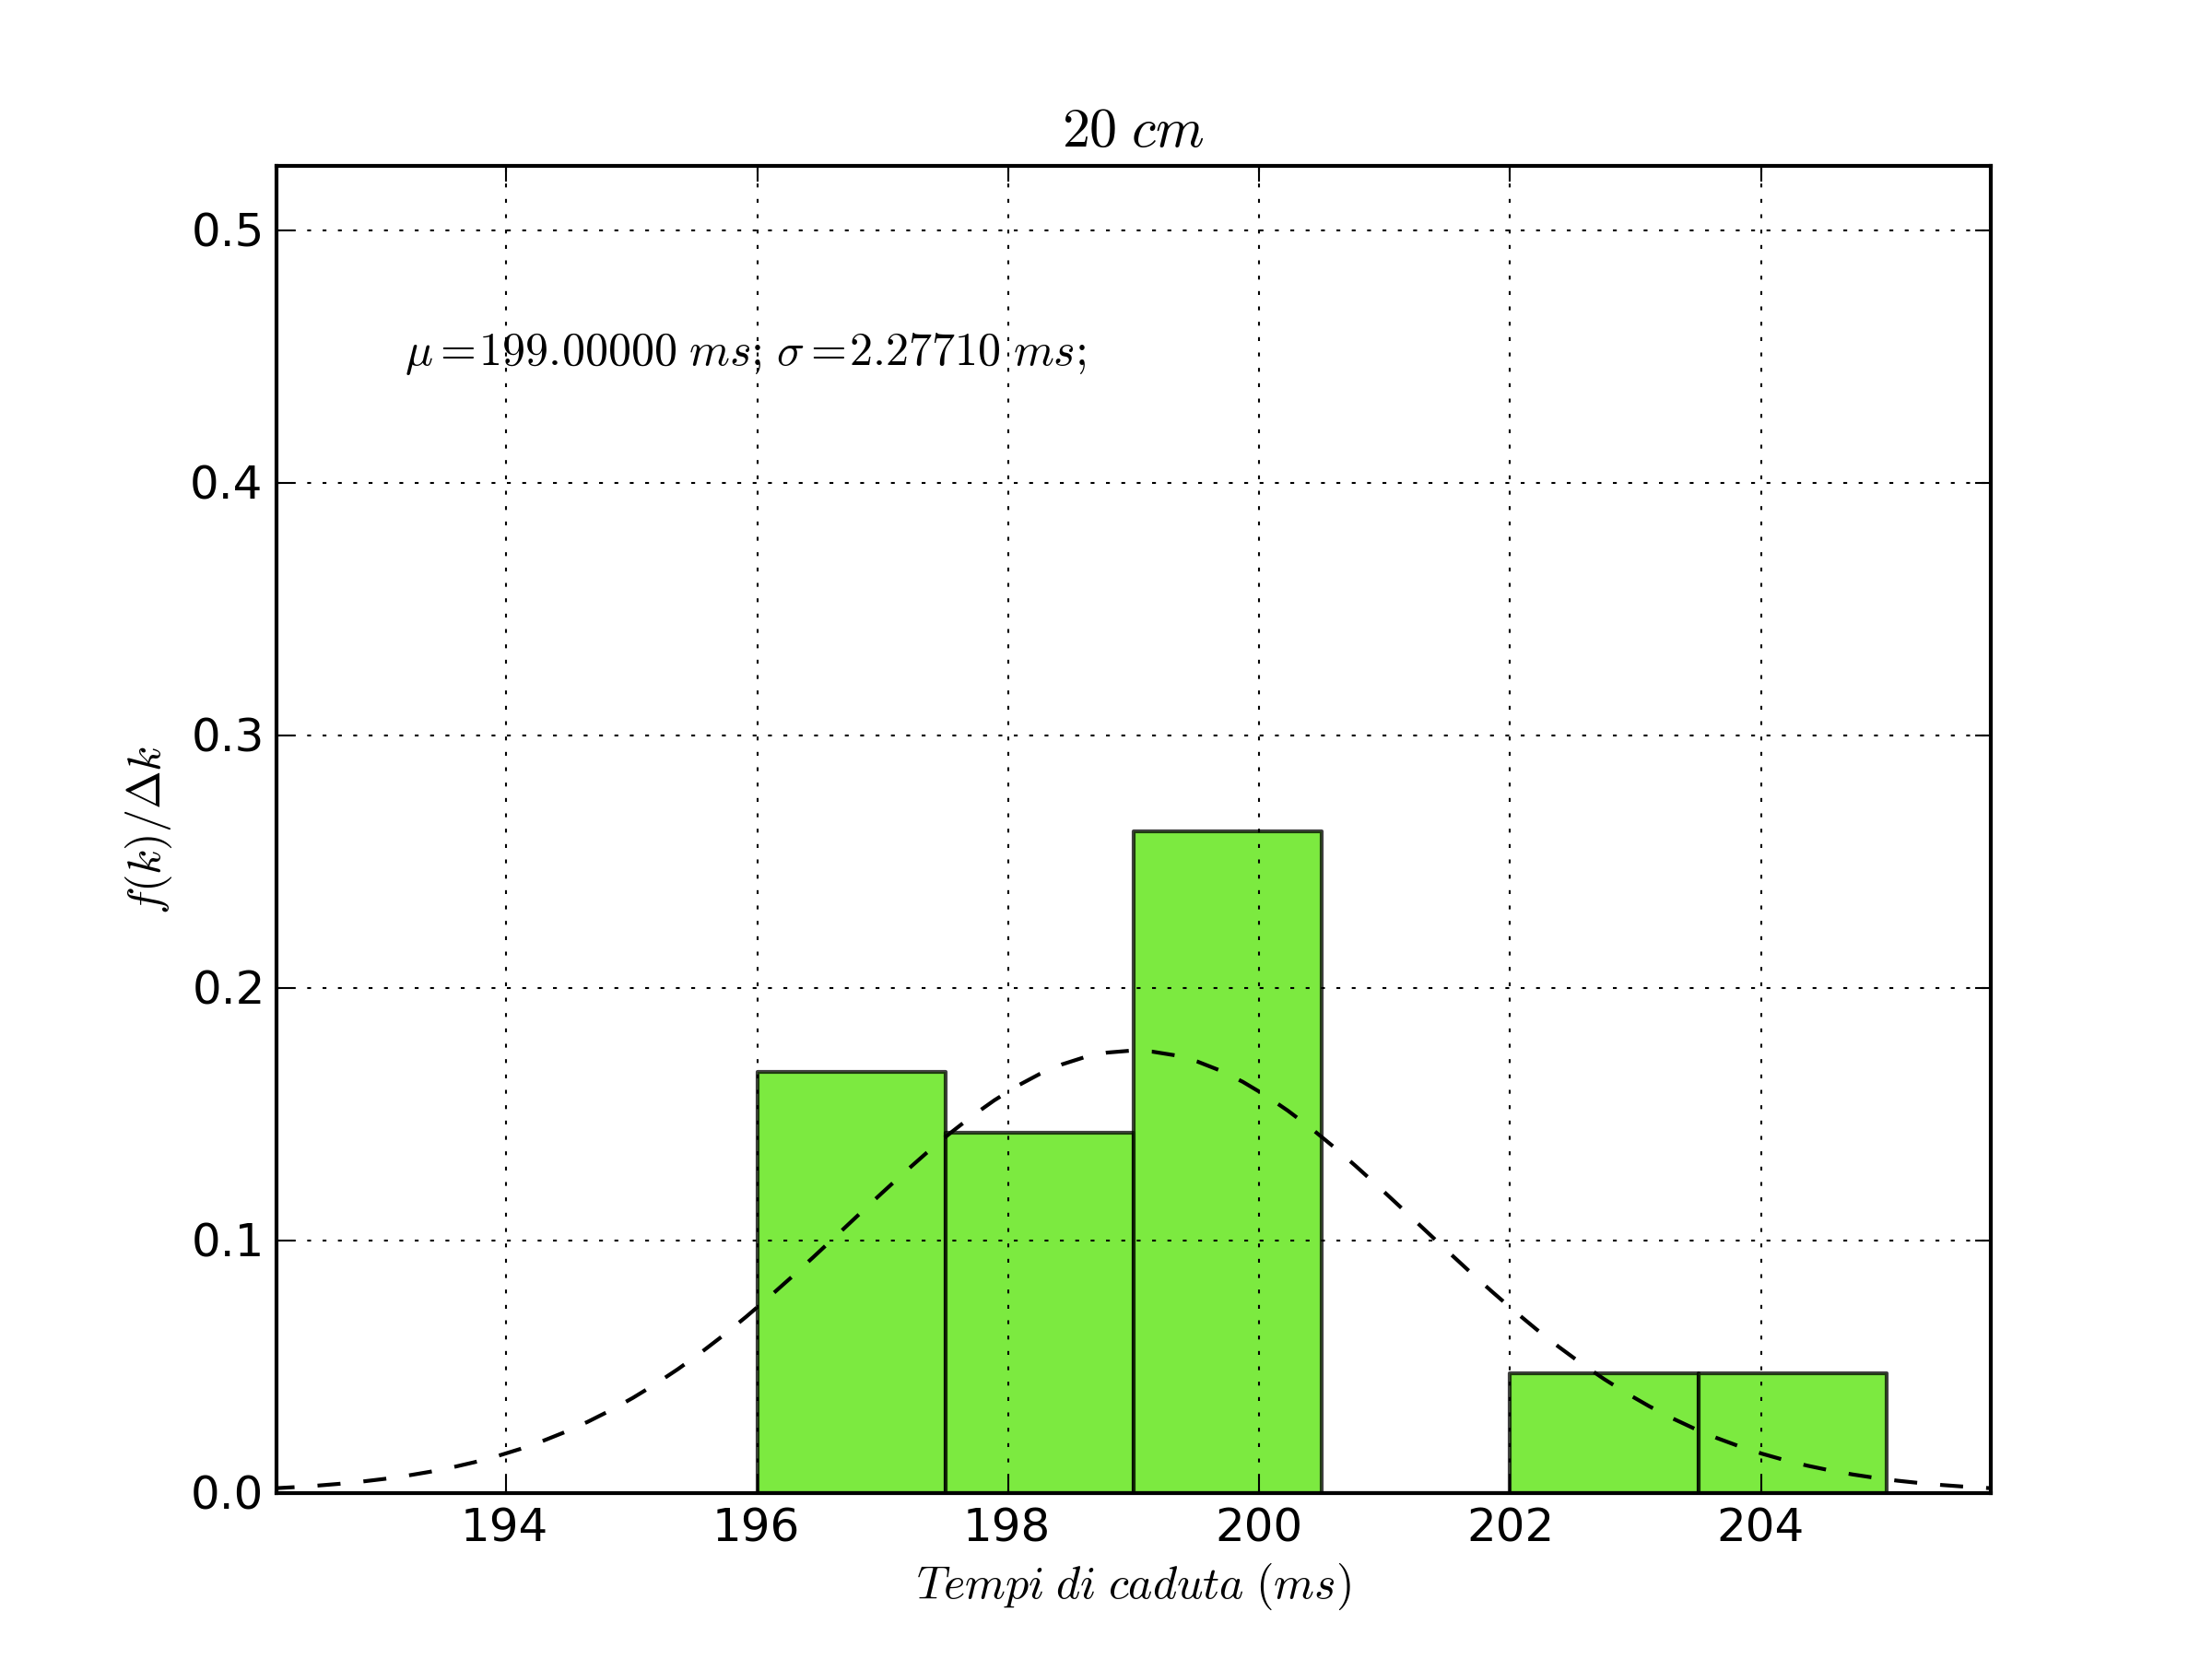
\includegraphics[scale=0.75]{../grafici/20cm.png}
$$\sigma_{\bar{x}} = 0.430\ ms$$
$$\mathrm{Stima\ di\ g} = 10.10\ m/s^2$$
$$\mathrm{Stima\ (corretta)\ di\ g} = 9.80\ m/s^2 $$
$$\frac{\Delta g_c}{g} = 0.00072$$
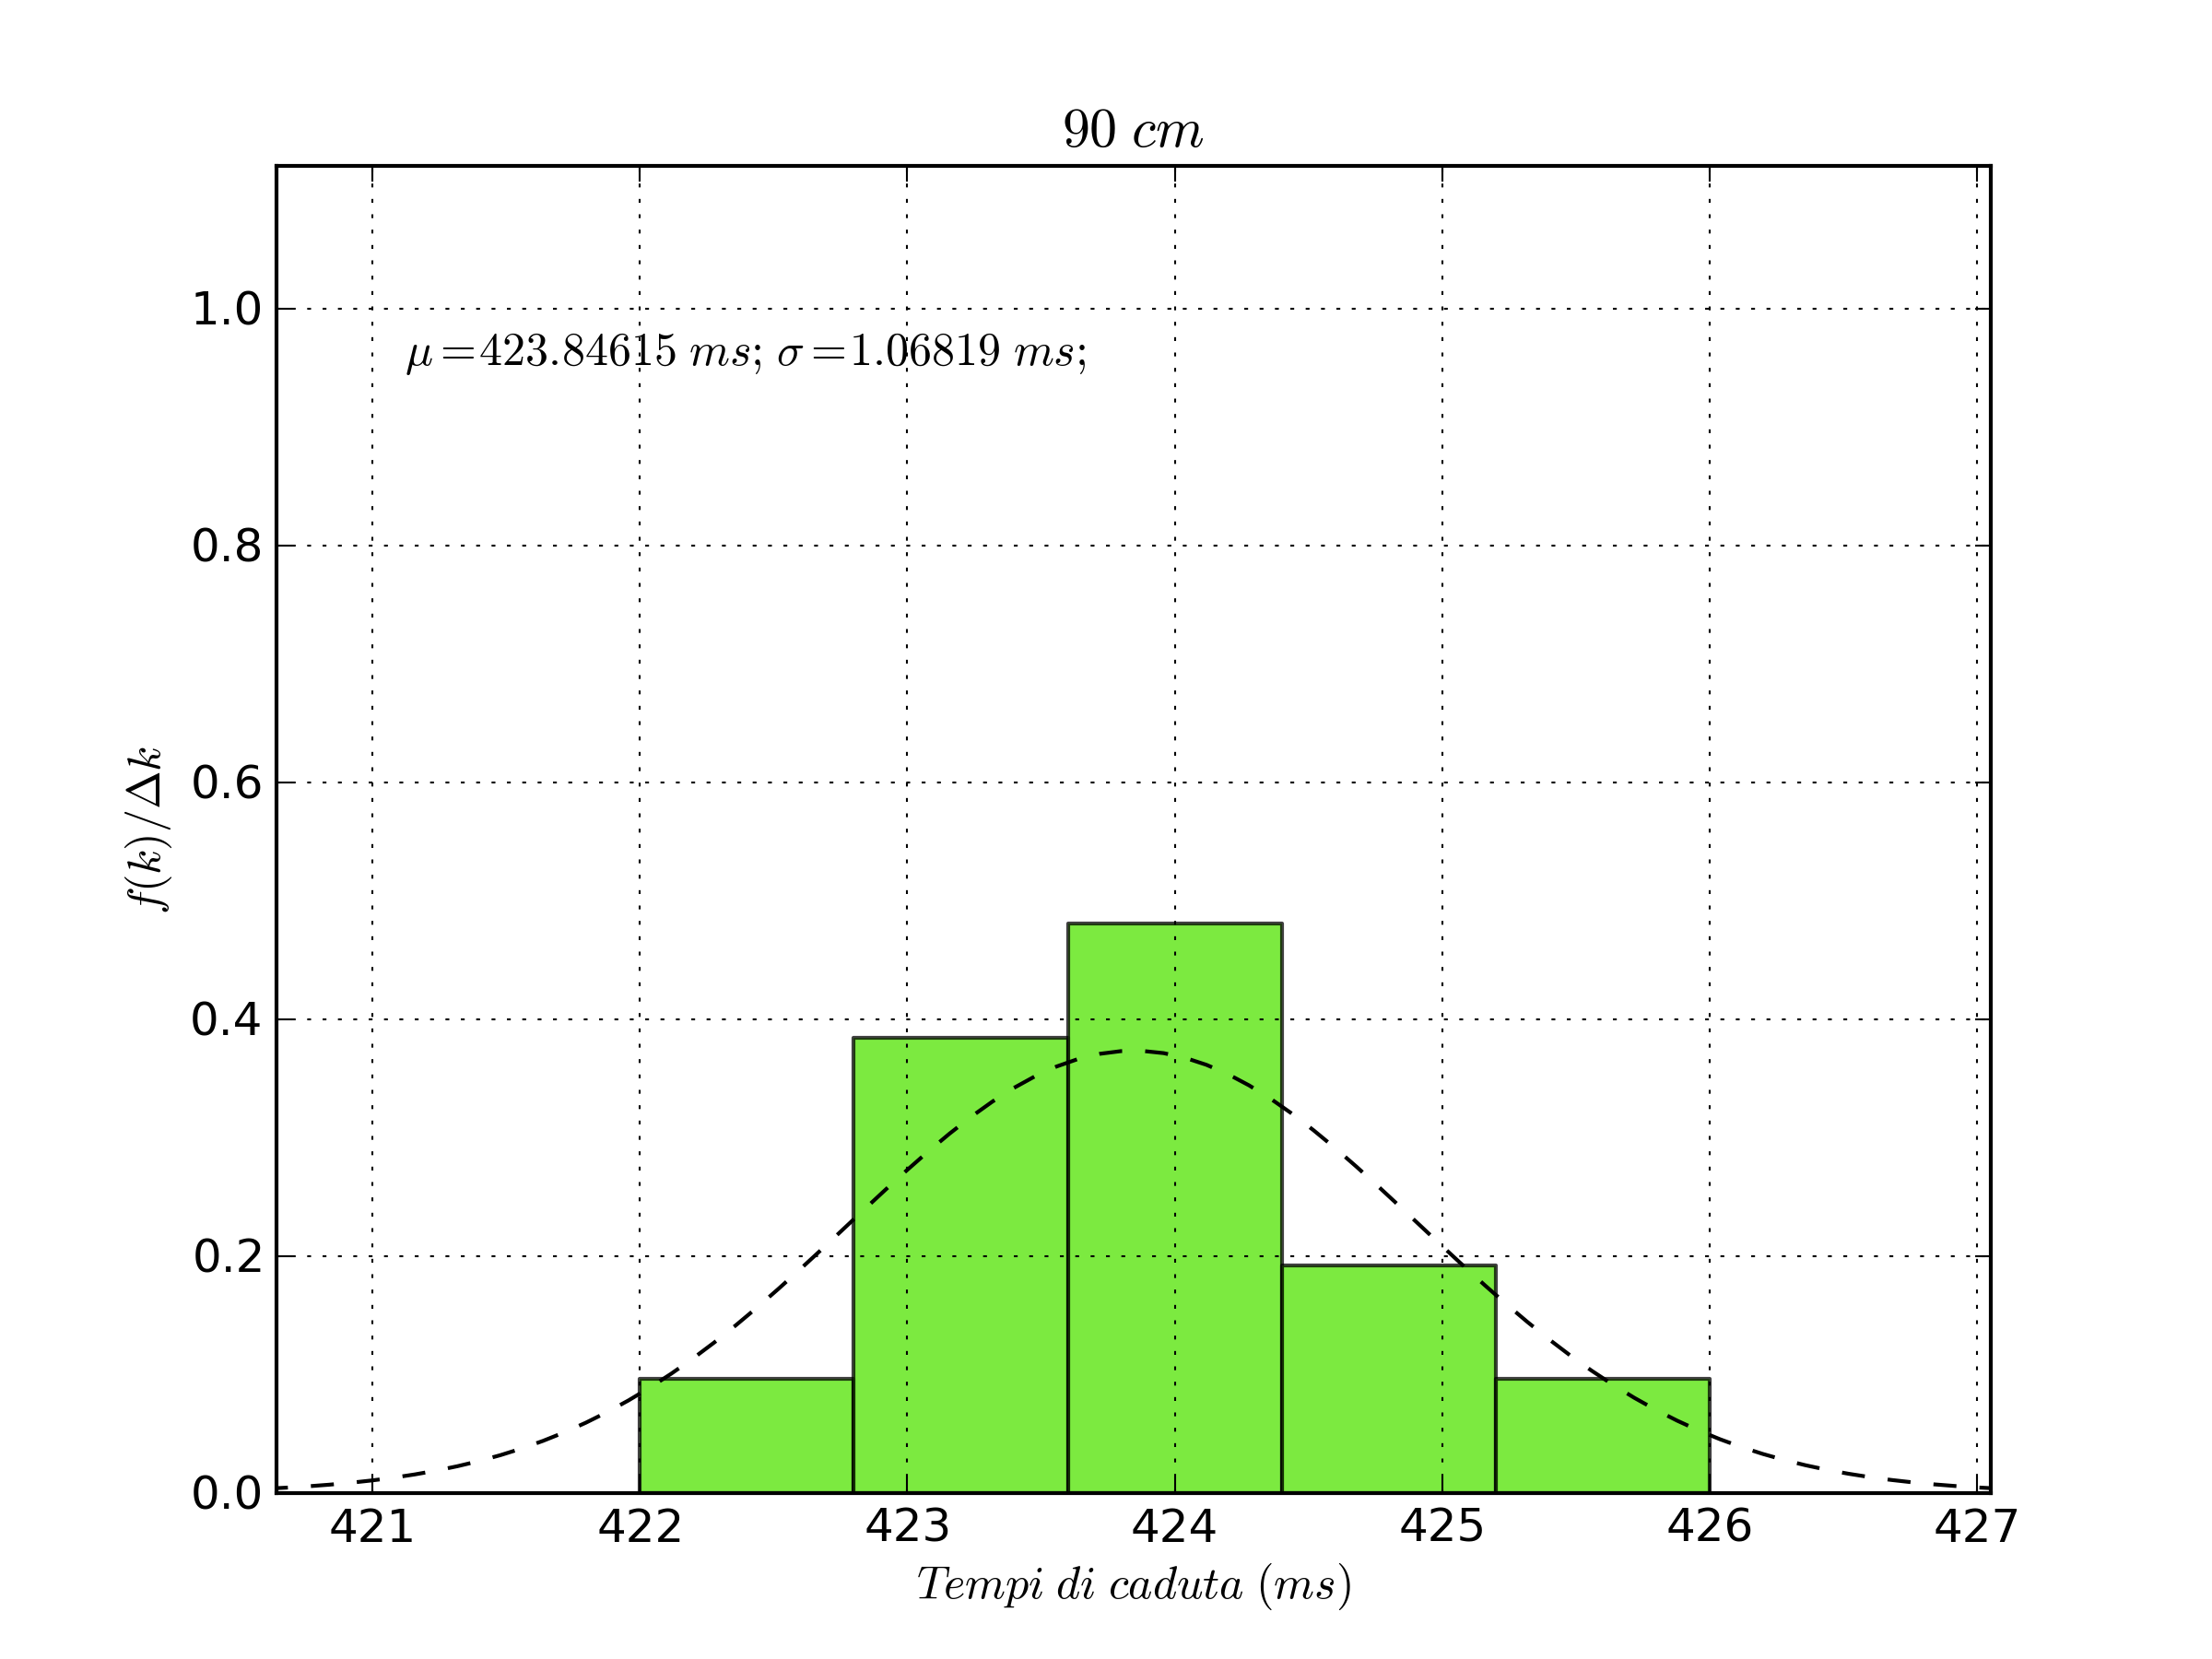
\includegraphics[scale=0.75]{../grafici/90cm.png}
$$\sigma_{\bar{x}} = 0.296\ ms $$
$$\mathrm{Stima\ di\ g} = 10.02\ m/s^2$$
$$\mathrm{Stima\ (corretta)\ di\ g} = 9.88\ m/s^2 $$
$$\frac{\Delta g_c}{g} = 0.00707$$
\end{center}

La correzione applicata è di 3 ms aggiunti al tempo segnato dal cronometro. Non avendo dati più precisi sulla costruzione del cronometro stesso, assumiamo questo tempo come [delay]... scrivi meglio!

\begin{center}
\begin{tabular}{c|c|c|c|c}
$h$ (m) & $g$ (m/s$^2$) & $g_c$ (m/s$^2$) & $\Delta g/g$ & $\Delta g_c/g$\\
\midrule
0.20 & 10.10 & 9.80 & 0.02964 & 0.00072 \\
0.35 & 10.07 & 9.85 & 0.02659 & 0.00362 \\
0.50 & 10.04 & 9.85 & 0.02354 & 0.00435 \\
0.60 & 10.05 & 9.88 & 0.02475 & 0.00718 \\
0.90 & 10.02 & 9.88 & 0.02138 & 0.00707 \\
\end{tabular}
\end{center}


\section{Conclusioni}
%
\chapter{Tubo di risonanza}

\section{Introduzione}

\section{Strumentazione}
\subsubsection{Tubo aperto contente aria}
Dati geometrici tubo:\\
$L = 90\pm 0.5\ cm$\\
$d = 3.9\pm 0.1\ cm$\\
con $L$ lunghezza e $d$ diametro del tubo.

\section{Tubo aperto contenente aria}
Cerchiamo le frequenze cui corrisponde, sullo schermo dell'oscilloscopio, il segnale massimo: in tal caso si ha la condizione di risonanza. Vogliamo verificare che tali valori stiano fra loro come multipli interi, secondo la legge:

\begin{equation} \label{eq:gianni}
\nu_n= n\frac{v}{2L} \hspace{3cm} n\in\mathbb{N} = \lbrace 1,2,3 \dots \rbrace
\end{equation}
con $v$ velocità del suono nel mezzo.
\\
Di seguito i dati raccolti:
\begin{center}
\begin{tabular}{c|c|c|c|c|c}
$\nu$ (Hz) & 185 & 370 & 558 & 930 & 1320 \\
\midrule
$n$ & 1 & 2 & 3 & 5 & 7\\
\end{tabular}
\end{center}
Interpoliamo i dati con una retta, usando il metodo dei minimi quadrati. Poniamo $x_i=n_i$, $y_i=\nu_i$ ed $m=\displaystyle{\frac{v}{2L}}$. Per stabilire l'errore sulle $y$, ossia sulle frequenze, si opera ad una analisi sperimentale della sensibilità dell'oscilloscopio; si verifica che all'interno di un intervallo minore di 10 Hz lo strumento non è in grado di distinguere ulteriori variazioni nella lettura delle frequenze: se ne ricava che l'incertezza relativa alle misure è di $\pm5 Hz$.

\begin{center}

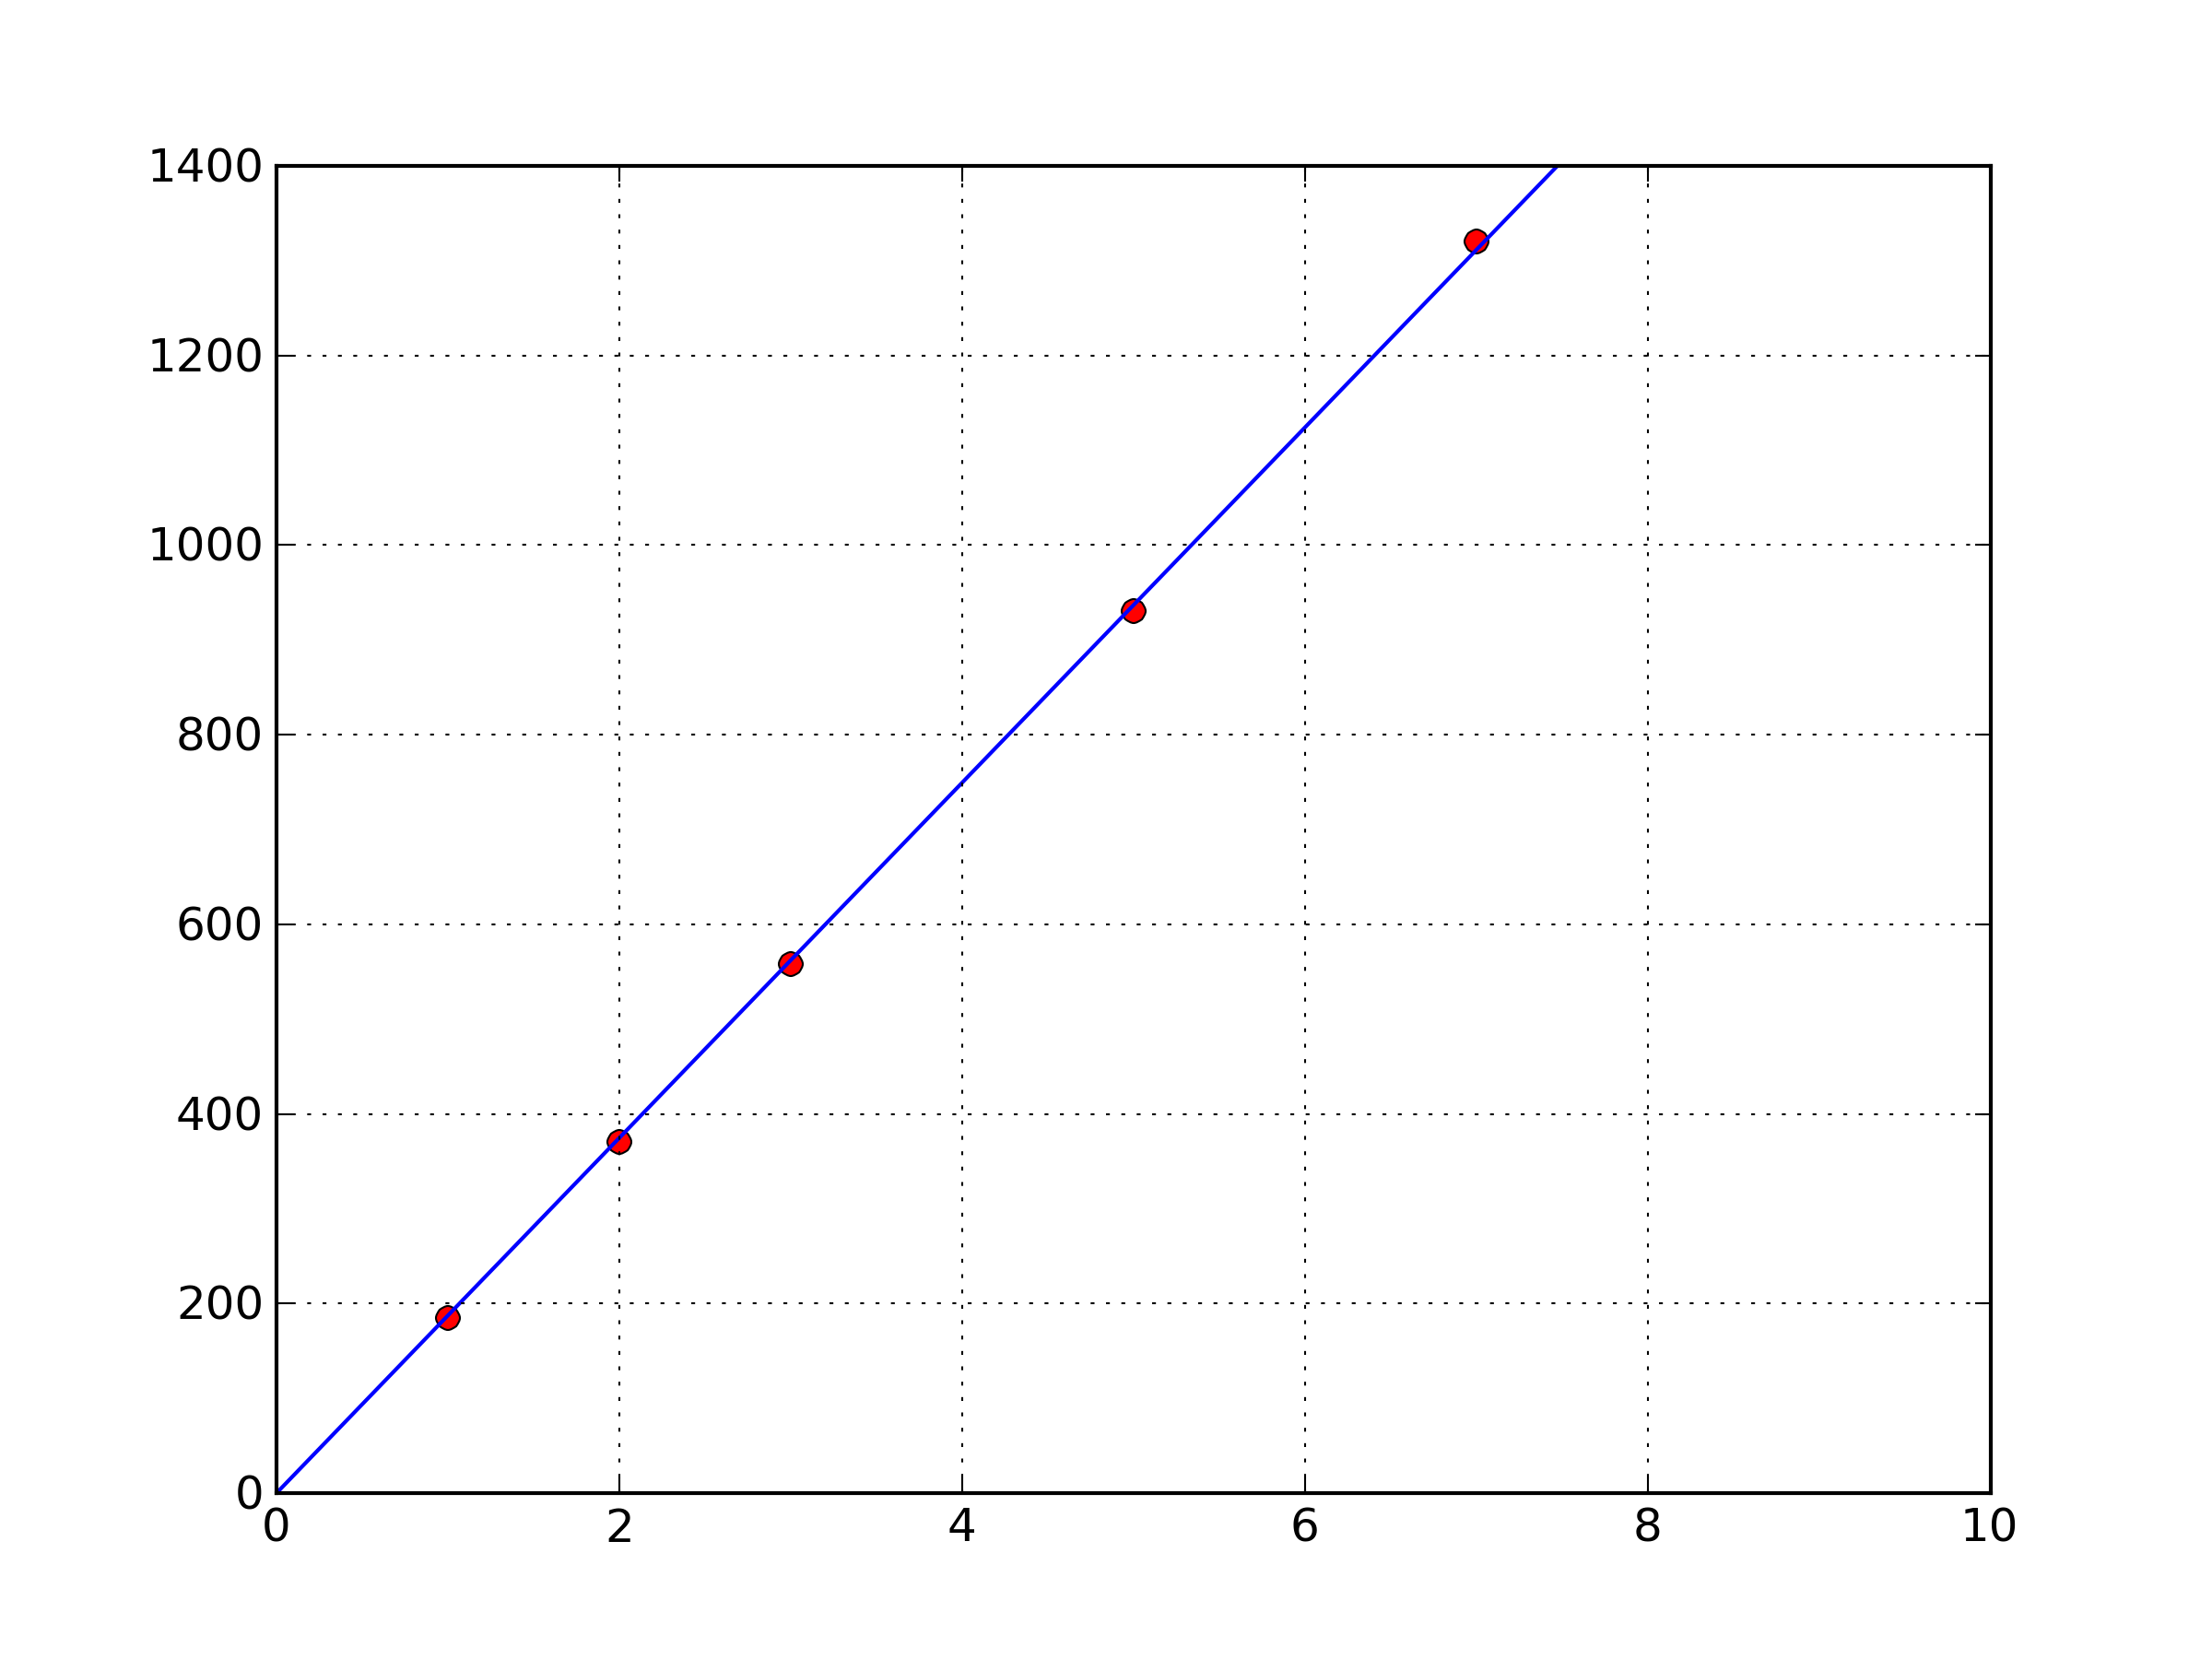
\includegraphics[scale=0.5]{../grafici/tubo/tubo1.png}

$m = 187\pm 1\ s^{-1}$\hspace{1cm}\footnote{L'incertezza su $m$ è data da: $$\sigma_m=\frac{\sigma_y}{\sqrt{\sum{x_i^2}}}$$}
\end{center}

Verifichiamo l'accordo tra la funzione ed i dati sperimentiali con un test del $\chi^2$, ponendo la soglia di accettabilità al 5\%.
\begin{equation}\label{chi2}
\chi^2=\displaystyle{\frac{\sum{(y_i-mx_i)^2}}{\sigma_{y}^2}}
\end{equation}

ponedo $\sigma_{y_i}=5\ Hz$ e $d=4$ otteniamo: $\tilde{\chi}^2=1,75$. Allora la probabilità che $\chi^2\geq\tilde{\chi}^2$ è del 13\%, il che conferma la correttezza delle ipotesi fatte.\\
\\
Tuttavia per un tubo aperto reale, la posizione di nodi e antinodi dipende anche dal diametro del tubo, secondo la legge:
$$\frac{n\lambda}{2}=L+0.8d$$ pertanto, prima di calcolare $v$ dal valore di $m$ apportiamo la seguente correzione:
$$ L_c = (90\ cm)+(0.8)(3.9\ cm) = 93.12\ cm = 0.93 m $$
Si ricava dunque che $$v=2L_cm=348\pm0.02\ m/s$$
\\
L'errore è stato ricavato dalla propagazione degli errori sulle lunghezze e sull'interpolazione:
$$\sigma_{L+0.8D}=\sqrt{((\sigma_L)^2+(0.8\sigma_D)^2}=0.55\ cm$$
$$\sigma_v= \sigma_{2mL_c}= 2\sqrt{\left(\frac{\sigma_m}{m}\right)^2+\left(\frac{\sigma_{L_{c}}}{L_c}\right)^2}= 0.02\ m/s$$


%Si può ricavare $v$ direttamente dalla \ref{eq:gianni} (con la correzione), sostituendo a $\nu$ la frequenza fondamentale $\nu_0 = 185$ Hz

%$$ v = 2L_c\frac{\nu}{n} = 344.544\pm9.39\ m/s$$ 
Confrontiamo il valore ottenuto con quello previsto dalla legge:
\begin{equation}
v=\sqrt{\frac{\gamma R T}{M}} = 348\ m/s
\end{equation}
con $\gamma=\displaystyle{\frac{C_p}{C_v}}=\frac{7}{5}$ (gas biatomico), $R=8.31\ J/K mol$, $T=293\ K$, $M= 0.028\ kg/mol$ (massa molare dell'azoto $N$).


\subsection{Ventri e nodi}
Posta una frequenza corrispondente a $n>1$ ($n=2, n=3$), spostiamo all'interno del tubo il microfono e cerchiamo i punti corrispondenti a ventri e nodi (posizione rispetto all'inizio del tubo).

\begin{center}
\begin{tabular}{r r r r}

\multicolumn{2}{c}{$\nu$ = 370 Hz}& \multicolumn{2}{c}{$\nu$ = 558 Hz}\\
\textit{nodo 1}:& 0 cm & \hspace{2cm}\textit{nodo 1}:& 0 cm\\
\textit{ventre 1}:& 22.5 cm & \hspace{2cm}\textit{ventre 2}:& 15 cm\\
\textit{nodo 2}:& 45 cm &\hspace{2cm}\textit{nodo 2}:& 30 cm\\
\textit{ventre 2}:& 67.5 cm &\hspace{2cm}\textit{ventre 3}:& 45 cm\\
\textit{nodo 3}:& 90 cm &\hspace{2cm} \textit{nodo 3}:& 60 cm\\
& & \textit{ventre 4}:& 75 cm \\
& & \textit{nodo 4}:& 90 cm \\
\end{tabular}
\end{center}

Si verifica che essi corrispondono a quanto previsto dalla \ref{frequenza}: per $n=2$ si hanno tre nodi (uno all'inizio, uno alla fine ed uno al centro della corda) e due ventri (nei punti medi dei segmenti congiungenti due nodi consecutivi); analogalmente avviene per $n=3$, in cui si hanno 5 nodi e 3 ventri. \footnote{Abbiamo omesso in tabella di riportare tutte le incertezze, per renderla più leggibile. La precisione del metro a nastro è di $\pm1\ mm$.}

\section{Tubo chiuso ad una estremità, contenente aria}

La condizione per l'instaurarsi di onde stazionarie in un tubo chiuso ad una estremità è data dalla relazione:
\\
\begin{equation}
 L=(2n-1)\frac{\lambda}{4}
\end{equation}
\begin{equation}\label{freq2}
\nu=\frac{(2n-1)}{L}v
\end{equation}
Operativamente, abbiamo risolto l'equazione soprastante rispetto a $n$.

$$ n = \frac{2L_c\nu}{v} + \frac{1}{2} $$
Verifichiamo, come nel caso del tubo aperto, che le frequenze di risonanza stanno fra loro come multipli interi: 

\textbf{L = 90 cm}
\\
\begin{center}
\begin{tabular}{c|c|c|c|c|c}
$\nu$ (Hz) & 285 & 475 & 670 & 860 & 1050 \\
\midrule
$n$ & 2 & 3 & 4 & 5 & 6 \\
\end{tabular}
\end{center}


\begin{center}
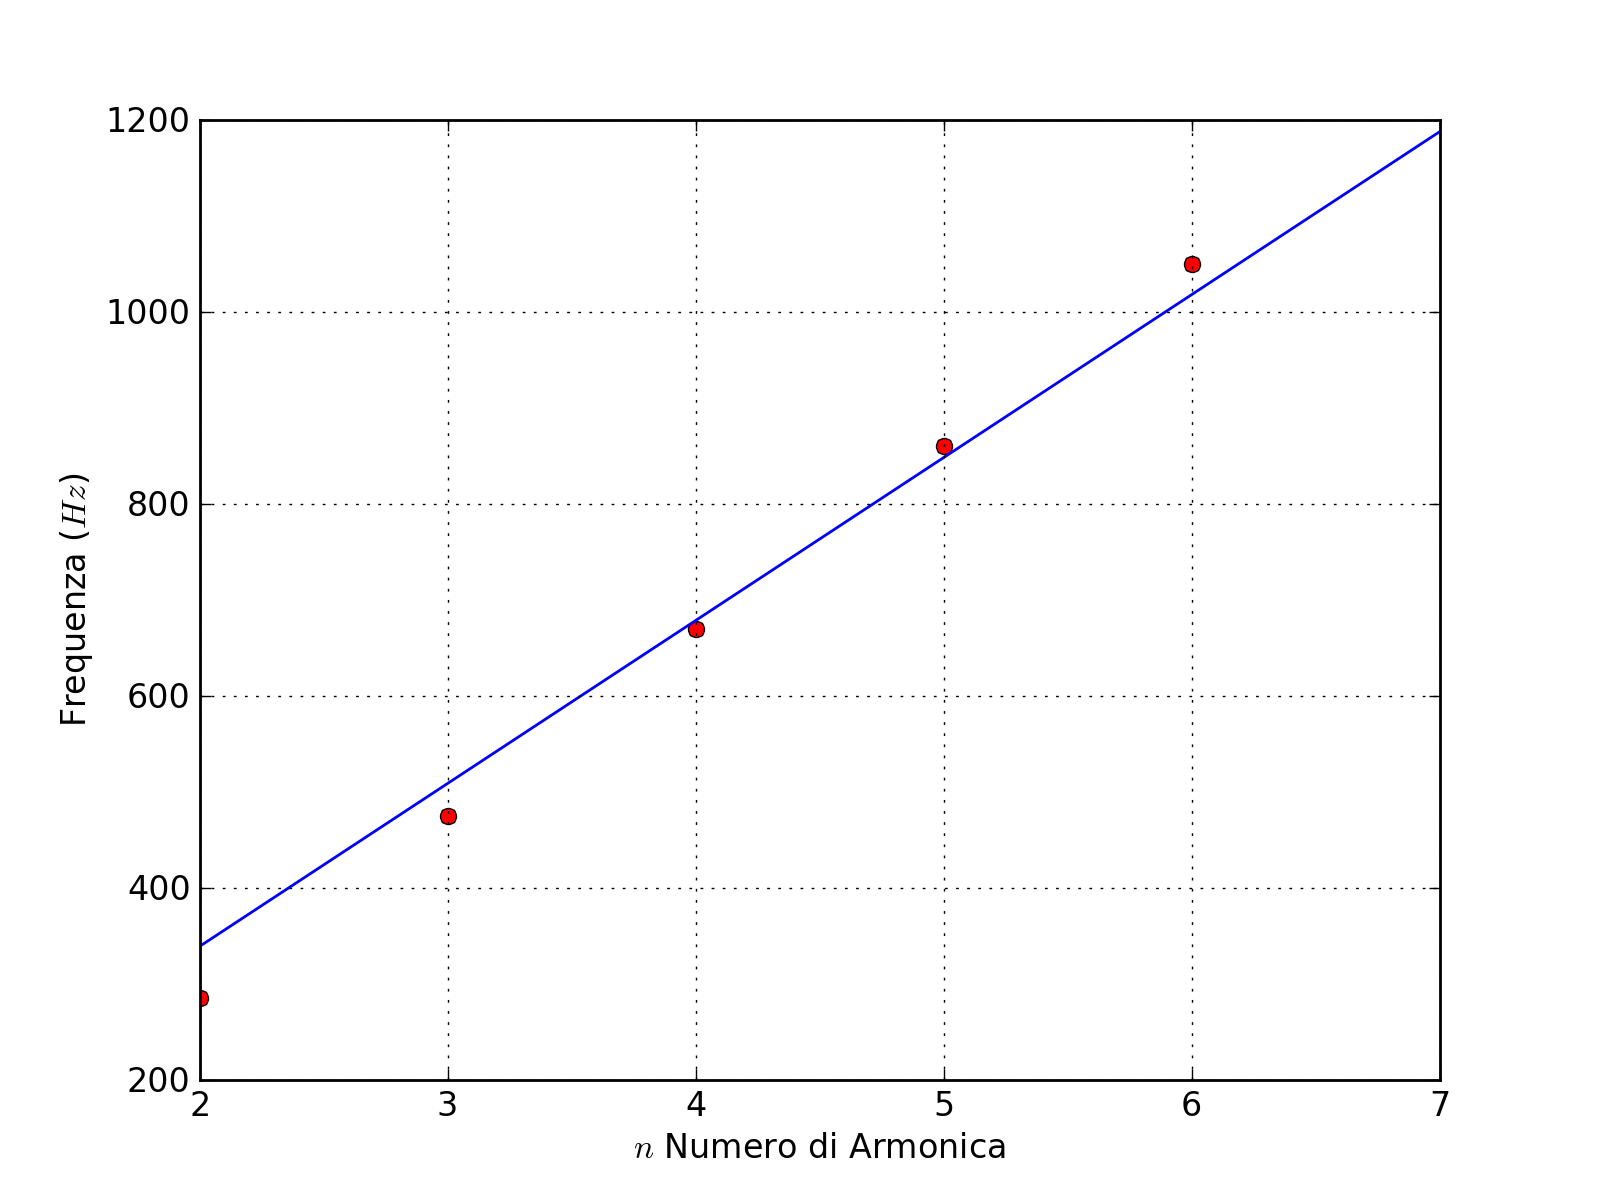
\includegraphics[scale=0.5]{../grafici/tubo/tubo2.png}

$m = v = 169\pm 1\ m/s$
\\

$P(\tilde{\chi}^2\geq\tilde{\chi_0}^2)=8\%$
\end{center}

\begin{center}
$\nu_0$= 475 Hz\\
\begin{tabular}{r r}
\textit{nodo 1}: & 0 cm\\
\textit{ventre 2}: & 17 cm\\
\textit{nodo 3}: & 34 cm\\
\textit{ventre 4}: & 53 cm\\
\textit{nodo 5}: & 70 cm\\
\end{tabular}
\end{center}

\subsection{Onda quadra}
La velocità del suono all'interno di un gas può essere misurata anche con un secondo metodo. Utilizzando un impulso a onda quadra e divendo la distanza totale percorsa per il tempo tra i due impulsi, otteniamo la velocità.  Per migliorare la precisione della nostra misura, abbiamo portato la risoluzione dello schermo dell'oscilloscipio ad 1 $\mu s$, in modo da poter discernere con più chiarezza la distanza tra i picchi nel grafico tempo-spazio.
Il $\Delta t$ misurato è di $4.98 \cdot 10^{-6} \ s$ e la lunghezza totale percorsa dall'impulso è $174 cm$ (2 volte la lunghezza del tubo meno la lunghezza del microfono e dello stantuffo). Ottieniamo quindi una velocità di :
$$v = 349 \pm 4 \ m/s$$
\\
con $$\sigma_v=\sqrt{\left(\frac{\sigma_t}{t}\right)^2+\left(\frac{\sigma_l}{L} \right)^2} \cdot v$$
Per la propagazione del suono nell'aria. Nel tubo contenente una miscela di $Kr$ (Kripton) e aria, con $L_{tubo} = 147 cm$ troviamo invece una velocità di $305 \pm 2\ m/s$. 

\subsection{Tubo a lunghezza variabile}
Abbiamo infine verificato la dipendenza delle frequenze di risonanza dalla lunghezza del tubo.

\begin{center}
\begin{tabular}{*{5}{c|}c}
L (cm) & 60 & 65 & 70 & 75 & 80 \\
\midrule
$\nu$ (Hz) &415 & 380 & 365 & 340 & 315\\
\end{tabular}
\end{center}
Interpoliamo i dati con l'equazione:
\begin{equation}\label{tubochiuso}
\nu=\frac{(2n-1)}{L}v
\end{equation} 
usando il metodo dei minimi quadrati. Nel nostro caso la \ref{tubochiuso}, avendo $n=1$, si presenta nella forma più semmplice:
$$\nu=\frac{v}{L}$$
Poniamo $x_i=1/L_i$, $y_i=\nu_i$ ed $m=v$.

\begin{center}
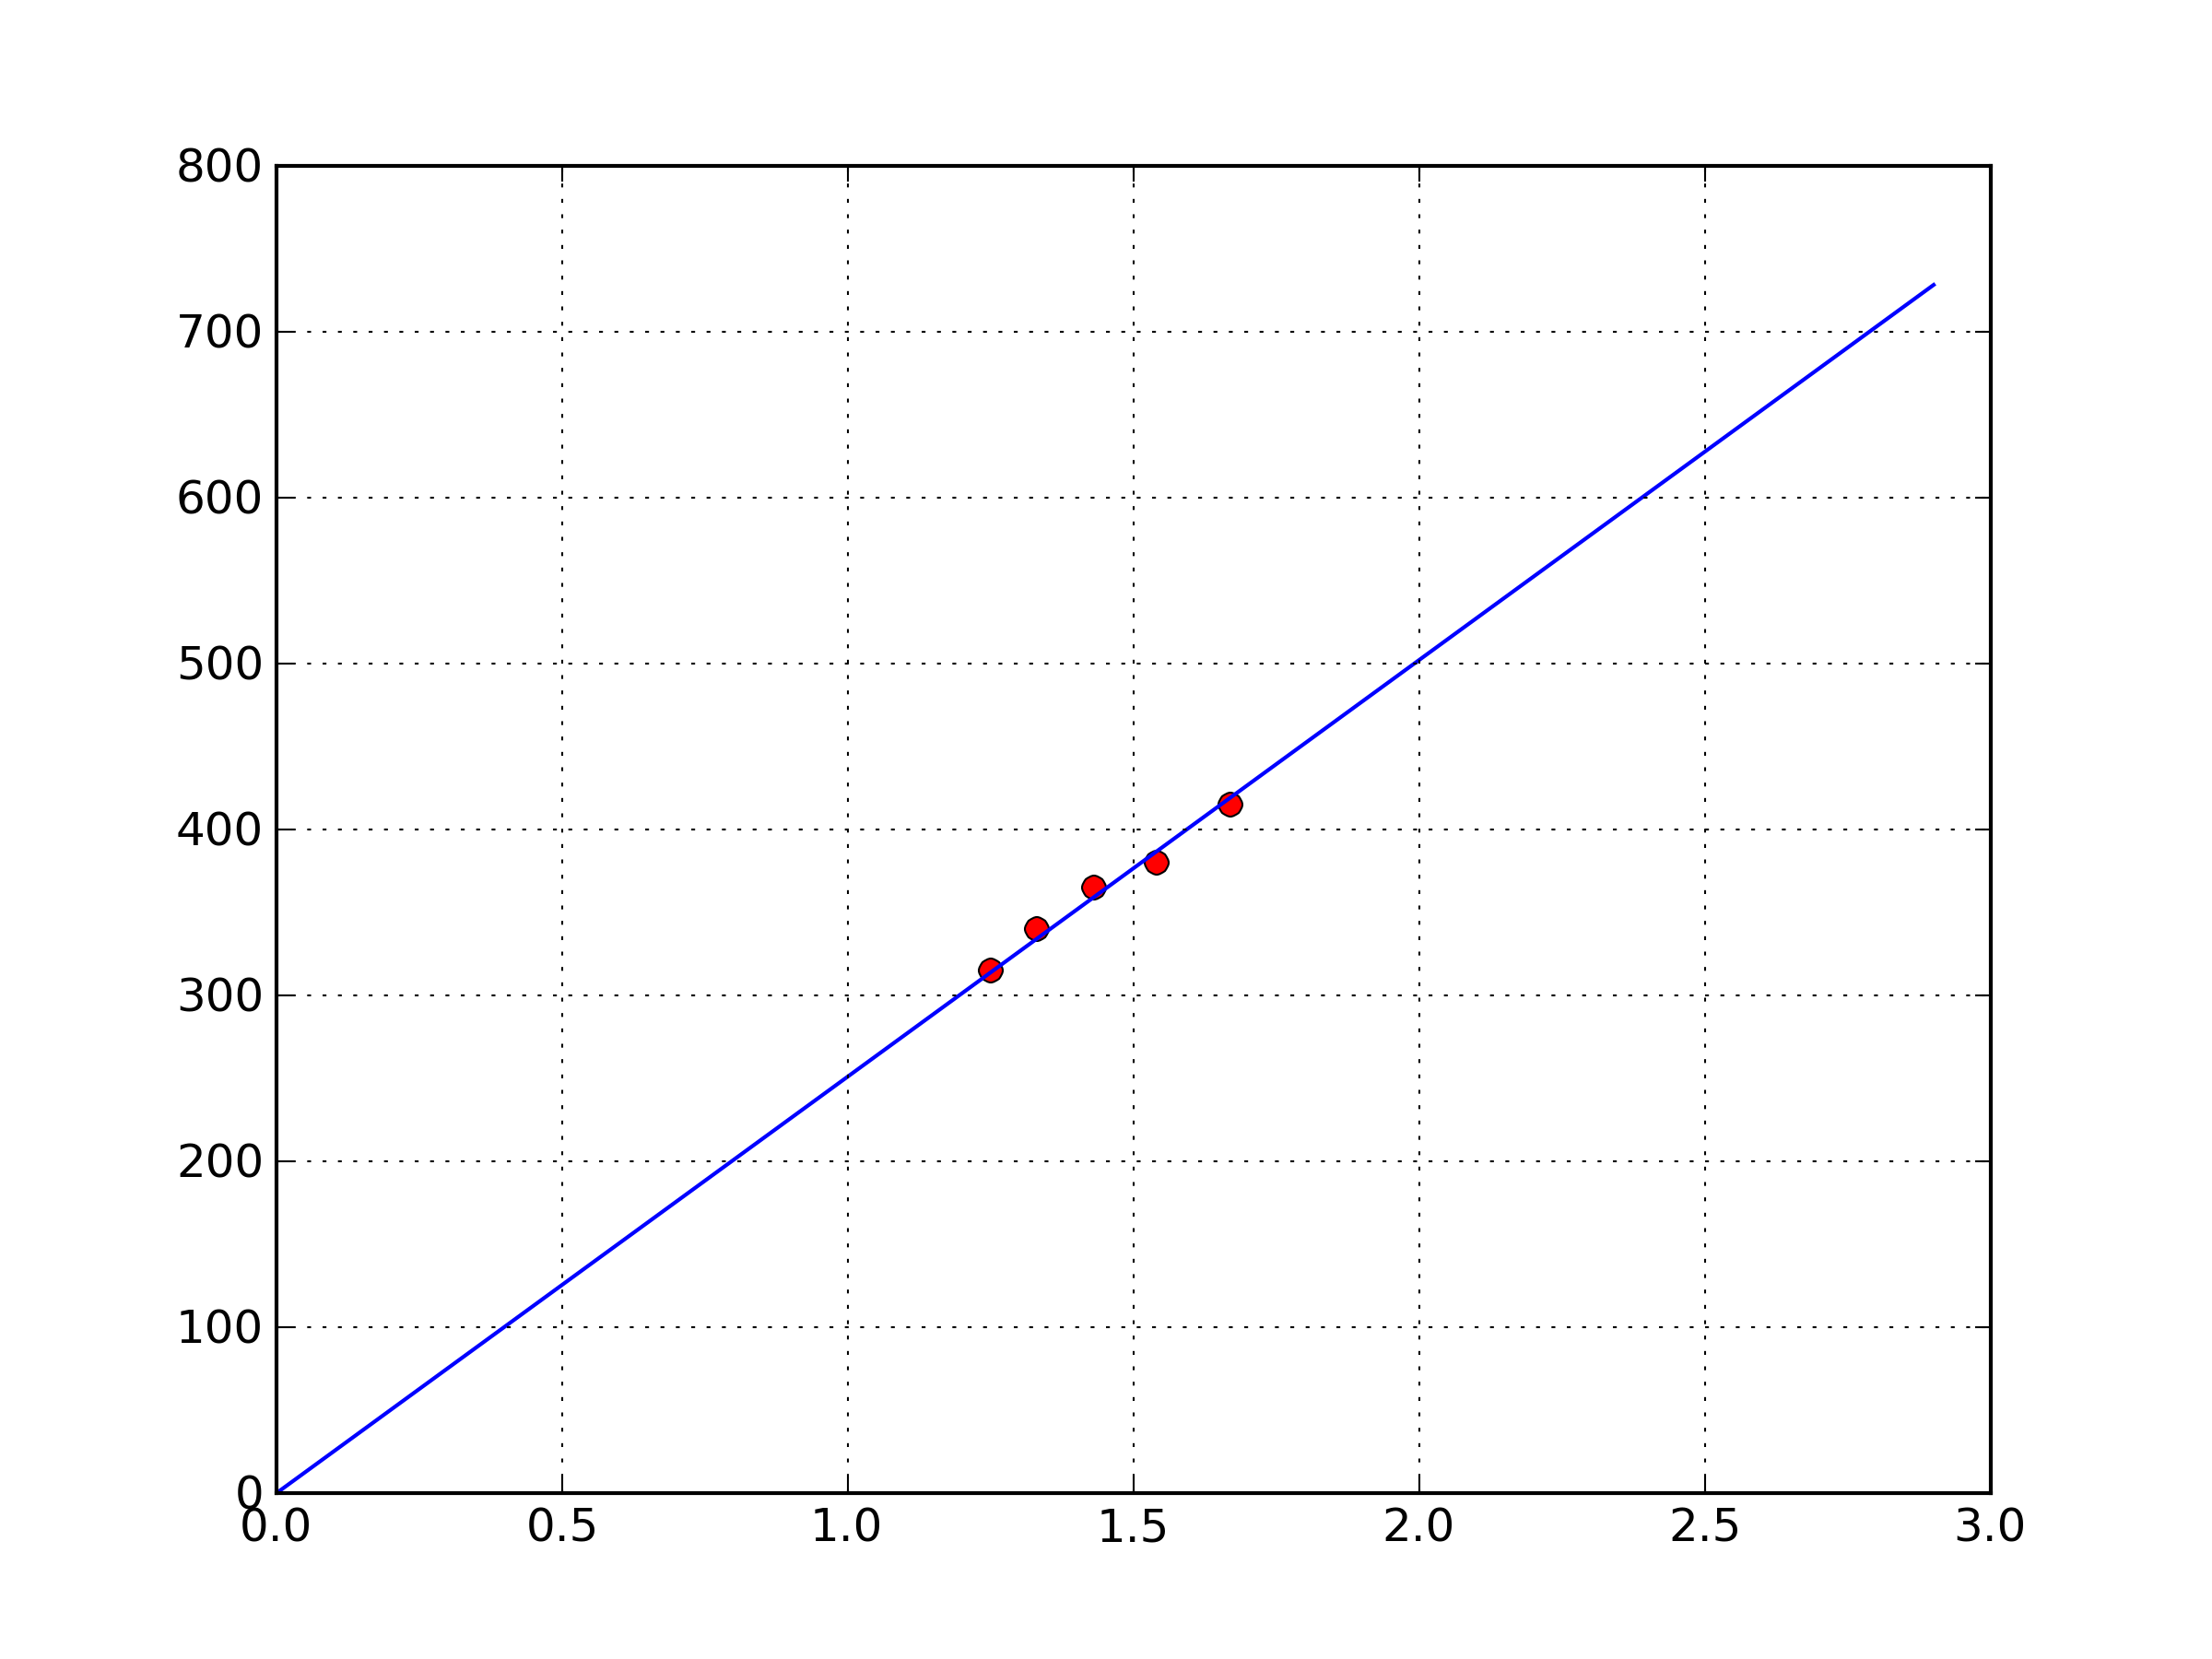
\includegraphics[scale=0.5]{../grafici/tubo/tubo3.png}

$m = v = 251\pm 1\ m/s$
\end{center}

\section{Tubo chiuso da ambo i lati, contenente Kripton}

$L_{tubo}$ = 147 cm\\
$D_{tubo}$ = 15 cm
$\nu$ = 75.7 Hz
 
\begin{center}
\begin{tabular}{c|c|c|c|c|c}
$\nu$ (Hz) & 102 & 204 & 312 & 415 & 518 \\
\midrule
$n$ & 1 & 2 & 3 & 4 & 5\\
\end{tabular}
\end{center}
Interpolando i dati tramite la funzione lineare 7.1 (con correzione) otteniamo:

$$ m_2 = 104 \pm 0.5 \ Hz  $$ 
\\
Da questa $m$, tramite il procedimento illustrato in precedenza, calcoliamo: 
$$v = 308.4\pm0.5\ m/s $$
\\
La seguente relazione:
$$v=\sqrt{\frac{\gamma RT}{M}}$$
\\
con $\gamma = \frac{C_p}{C_v}$, $R$ è la costante dei gas, $M$ la massa molare e $T$ la temperatura in gradi Kelvin, ci fornisce il valore teorico della velocità di propagazione di un'onda sonora in relazione alle caratteristiche del mezzo. 
Il risultato atteso è dunque $v=222.7 m/s$. Confrontando questo risultato con il valore misurato sperimentalmente siamo giunti alla conclusione che all'interno del tubo vi è presente una miscela di Kripton e aria $\simeq 50\%.$




%
\chapter{Molla}

\section{Introduzione}
Oggetto di studio è la verifica della legge di Hooke, che lega la deformazione che si manifesta su un corpo soggetto ad una forza elastica all'intensità della forza stessa:
\begin{equation}\label{Hooke}
F=-kx
\end{equation}
Nello specifico delle nostre analisi, ci occuperemo della forza di richiamo di una molla. $x$, che compare nella \ref{Hooke} è l'allungamento della molla dalla posizione di equilibrio.
Noto il valore della forza (nel nostro caso si tratterà sempre della forza peso $F=Mg$), si può inoltre determinare la costante di proporzionalità $k$, caratteristica di ciascuna molla.

\section{Strumenti}
La strumentazione si compone di un gancio cui si appende la molla di cui si vogliono studiare le caratteristiche, e nel punto corrispondente del tavolo (lungo la perpendicolare) si pone un sensore di posizione che trasmette i dati rilevati (allungamento) al computer, dove sono poi analizzati con il programma DataStudio.\\
\\
\begin{tabular}{c c c}
\textbf{Molla A} & \hspace{1.5cm} $L_A=0.430\ m$ & \hspace{1.5cm} $M_A=4.289\ g$\\
\\
\textbf{Molla B} & \hspace{1.5cm} $L_B=0.426\ m$ & \hspace{1.5cm} $M_B=4.029\ g$\\
\end{tabular}
\\
\\
Per la terza parte dell'esperimento ci siamo serviti di un disco di cartone di massa $M=2.5\ g$. 
\\
\\
Con $L_A$ ed $L_B$ lunghezze a riposo delle due molle.

\section{Misura statica}

La \ref{Hooke} implica che il rapporto tra l'allungamento della molla e la forza esercitata sia un valore costante:
$$k=\frac{Mg}{x}$$
Facendo variare le masse appese, verifichiamo dunque la validità della \ref{Hooke} e successivamente otteniamo il valore di $k_1$ e $k_2$ corrispondenti alle due molle.   
Di seguito in tabella i valori raccolti per le due molle.\footnote{I valori sono stati raccolti con una frequenza di campionamento di 10 $Hz$}
\footnote{Durante tutto l'esperimento gli errori associati alle interpolazioni si sono rivelati trascurabili (dell'ordine di $10^{-5}$ i più grandi), per cui ne abbiamo evitato anche la trascrizione.}

\begin{center}

\begin{tabular}{c c}
\textbf{Molla A} & \hspace{2cm} \textbf{Molla B}\\
\\
\begin{tabular}{c|c|c}
Massa ($kg$) & Misura L ($m$) & $\Delta L$ ($m$)\\
\midrule
0.200 & 0.422 & 0.008\\
0.250 & 0.420 & 0.010\\
0.300 & 0.418 & 0.012\\
0.400 & 0.414 & 0.016\\
0.450 & 0.412 & 0.018\\
0.500 & 0.410 & 0.020\\
0.550 & 0.408 & 0.022\\
0.600 & 0.406 & 0.024\\
0.650 & 0.404 & 0.026\\
0.700 & 0.402 & 0.028\\
\end{tabular}

& \hspace{2cm}

\begin{tabular}{c|c|c}
Massa ($kg$) & Misura L ($m$) & $\Delta L$ ($m$)\\
\midrule
0.200 & 0,424 & 0.002\\
0.250 & 0,422 & 0.004\\
0.300 & 0,420 & 0.006\\
0.400 & 0,416 & 0.001\\
0.450 & 0,413 & 0.013\\
0.500 & 0,411 & 0.015\\
0.550 & 0,409 & 0.017\\
0.600 & 0,407 & 0.002\\
0.650 & 0,404 & 0.022\\
0.700 & 0,402 & 0.024\\
\end{tabular}

\end{tabular}

\end{center}

%Grafici

\section{Misura dinamica}

\subsubsection{Procedimento e breve accenno di teoria}

Quando una molla viene spostata dalla propria posizione di equilibrio, essa esercita una forza di richiamo data dalla \ref{Hooke}. Se su di essa agisce anche la forza peso, si ha:
$$\displaystyle\sum{F}=Mg-kx$$
Dalla II legge di Newton, dividendo tutto per M ed esprimendo $g$ dalla \ref{Hooke} come $g=\displaystyle{\frac{kx_0}{M}}$, ricaviamo:

\begin{equation}
\frac{d^2x}{dt^2}+\frac{k}{M}(x-x_0)
\end{equation}

con $x_0=\displaystyle{\frac{Mg}{k}}$ posizione di equilibrio.\\
\\
Tale equazione descrive un moto armonico semplice, la cui legge del moto è data da:

\begin{equation}\label{eqmoto}
x(t)=x_0+Asin(\omega t+\phi)
\end{equation} 
il cui periodo, nel caso di molle con massa non trascurabile, è dato da:

\begin{equation}\label{periodo}
T=2\pi\sqrt{\frac{M+m/3}{k}}
\end{equation}  

A questo punto è facile determinare il valore di $k$. Sospendiamo dunque alla molla una massa, e discostatala dalla posizione di equilibrio la lasciamo libera di oscillare. Verifichiamo dal grafico tracciato in tempo relale dal programma DataStudio, sincronizzato alla fotocellula di posizione, che si tratti effettivamente di un moto armonico. Infine dai valori del quadrato del periodo, ottenuti mediante l'interpolazione con una sinusoidale, si ricava il valore di $k$. In questo caso si fa uso di una interpolazione con il metodo dei minimi quadrati, ponendo $x_i=M_i$, $y_i={T_i}^2$ ed $m=\displaystyle{\frac{4\pi^2}{k}}$. 

\subsubsection{Raccolta dati}

\begin{center}

\begin{tabular}{c c}
\textbf{Molla A} & \hspace{2cm} \textbf{Molla B}\\
\\
\begin{tabular}{c | c| c}
Massa ($g$) & Periodo ($s$) & Pulsazione ($rad/s$)\\
\midrule
400 & 0.274 & 22.93\\
600 & 0.340 & 18.48\\
800 & 0.374 & 16.80\\
\end{tabular}

& \hspace{2cm}

\begin{tabular}{c | c | c}
Massa ($g$) & Periodo ($s$) & Pulsazione ($rad/s$)\\
\midrule
500 & 0.312 & 20.14\\
700 & 0.364 & 17.26\\
900 & 0.409 & 15.36\\
\end{tabular}

\end{tabular}

\end{center}

I grafici mostrano la dipendeza lineare tra $T^2$ ed $M$.

%Grafici della dipendenza lineare (uno sotto molla A e l'altro sotto molla B)

Dall'interpolazione ricaviamo:
\begin{center}
\begin{tabular}{c c}
$m_A=0.182$ & \hspace{3cm} $m_B=0.188$\\ 
\\
$k_A=\displaystyle{\frac{4\pi^2}{m_A}}=216.9\ Nm$ & \hspace{3cm} $k_B=\displaystyle{\frac{4\pi^2}{m_B}}=210.0\ Nm$ \\
\end{tabular}
\end{center}

%Grafici dell'energia potenziale, en.cinetica ed energia potenziale.

\section{Moto armonico smorzato}

Fissando il disco di cartone all'estremità oscillante della molla, si aumenta l'effetto frenante dell'aria ($F=-bv$, con $b$ coefficiente di smorzamento).  
In tal caso si assiste ad una diminuzione dell'ampiezza di oscillazione, secondo la legge:
\begin{equation}\label{Asm}
A(t)=A_{max}exp[-b/2M)t]
\end{equation}
E la legge del moto diventa:
\begin{equation}
x(t)=A(t)\cos(\omega't-\phi)=A_{max}exp[-(b/2M)t]\cos(\omega't-\phi)
\end{equation}
con $\omega'^2=\omega^2-(b/2M)^2$.

Utilizziamo tale funzione per interpolare i dati e ricavare il valore della costante $b$, al variare di M.\footnote{I dati sono stati raccolti con una frequenza di campionamento di 40 $Hz$}
\begin{center}

\begin{tabular}{c c}
\textbf{Molla A} & \hspace{1cm} \textbf{Molla B}\\
\\
\begin{tabular}{c | c | c | c}
$\boldsymbol{M}$ ($kg$) & $\boldsymbol{T}$ ($s$) & $\boldsymbol{\omega'}$ ($rad/s$) & $\boldsymbol{b}$ ($kg/s$)\\
\midrule
0.400 & 0.284 & 22.113 & 0.0228\\
0.600 & 0.336 & 18.690 & 0.0329\\
0.800 & 0.381 & 16.483 & 0.0369\\
\end{tabular}

& \hspace{1cm}

\begin{tabular}{c | c | c | c}
$\boldsymbol{M}$ ($kg$) & $\boldsymbol{T}$ ($s$) & $\boldsymbol{\omega'}$ ($rad/s$) & $\boldsymbol{b}$ ($kg/s$)\\
\midrule
0.500 & 0.321 & 19.574 & 0.0262\\
0.900 & 0.416 & 15.096 & 0.0364\\
0.700 & 0.372 & 16.882 & 0.0291\\
\end{tabular}

\end{tabular}

\end{center}

\begin{center}

\begin{tabular}{c c}
$\bar{b}_A=\displaystyle{\frac{\sum{b_i}}{N}}=0.0309\ kg/s$ & \hspace{1cm} $\bar{b}_B=\displaystyle{\frac{\sum{b_i}}{N}}= 0.0306\ kg/s$\\
\\
$\sigma_{\bar{b}_A}=\displaystyle{\sqrt{\frac{\sum{(b_i-\bar{b})^2}}{N-1}}}=0.0073\ kg/s$ & \hspace{1cm} $\sigma_{\bar{b}_B}=\displaystyle{\sqrt{\frac{\sum{(b_i-\bar{b})^2}}{N-1}}}= 0.0053\ kg/s$\\
\end{tabular}

\end{center}

È inoltre possibile ricavare $\omega'$ direttamente dal periodo delle oscillazioni smorzate: confrontiamo i valori ottenuti con i due differenti metodi:

\begin{center}

\begin{tabular}{c c}
\textbf{Molla A} & \hspace{2cm} \textbf{Molla B}\\
\\
\begin{tabular}{c | c}
$\boldsymbol{\omega'_{interpolato}}$ ($rad/s$) & $\boldsymbol{\omega'_{calcolato}}$ ($rad/s$)\\
\midrule
22.113 & 22.123\\
18.690 & 18.699\\
16.483 & 16.491\\
\end{tabular}

& \hspace{1cm}

\begin{tabular}{c | c}
$\boldsymbol{\omega'_{interpolato}}$ ($rad/s$) & $\boldsymbol{\omega'_{calcolato}}$ ($rad/s$)\\
\midrule
19.574 & 19.573\\
15.096 & 15.103\\
16.882 & 16.890\\
\end{tabular}

\end{tabular}

\end{center}
\chapter{Corda Vibrante}

\section{Introduzione}

Obiettivo di questo esperimento è lo studio della propagazione di onde elastiche su una corda \textbf{fissata ad un estremo}, sotto l'azione di una forzante con andamento sinusoidale. \textbf{Verifichiamo} la dipendenza della frequenza dell'onda ($\nu_n$) \textbf{dalla lunghezza della corda, dalla sua massa lineare ($\mu$)} e dalla tensione ($T$) applicata su di essa.
\textbf{Tali grandezze sono infatti legate dalle seguenti relazioni:}
\begin{center}
\begin{tabular}{c c c}
$
v= \sqrt{\frac{T}{\mu}} 
$
&
\hspace{1cm}
$
v= \nu_{n} \lambda_n
$ 
&
\hspace{1cm}
$
\lambda_n= \frac{2L}{n} 
$
\\
\end{tabular}
\end{center}

da cui:

\begin{equation}
\nu_n=\frac{n}{2L}\sqrt{\frac{T}{\mu}}
\end{equation}

con $n$ numero intero, al cui variare corrispondono differenti armoniche.


\section{Strumenti}

La strumentazione di cui ci siamo serviti si componeva di due corde:\\

\begin{tabular}{c c c c}
\textbf{Corda A} & \hspace{1cm} $L_A= 2.46\ m$ & \hspace{1cm} $m_A=5.21\cdot10^{-3}\ kg$ & \hspace{1cm} $\mu_A= 2.12\cdot10^{-3}\ kg/m$\\
\textbf{Corda B} & \hspace{1cm} $L_B= 2.50\ m$ & \hspace{1cm} $m_B=1.63\cdot10^{-2}\ kg$ & \hspace{1cm} $\mu_B= 6.52\cdot10^{-3}\ kg/m$\\
\end{tabular} 
\\

La forzante è data da un oscillatore elettromeccanico, mentre la tensione è esercitata da pesetti appesi all'estremità libera della corda, sospesi attraverso una carrucola (come illustrato in \textbf{figura}). 
 

\section{Ricerca delle armoniche}

Nella prima parte dell'esperienza abbiamo verificato che le armoniche superiori sono date da multipli interi della frequenza fondamentale. A tal fine, dopo aver trovato la frequenza di risonanza \textbf{corrispondente ad $n=1$ (ossia la fondamentale)}, facendo variare la frequenza dell'oscillatore elettromeccanico e cercando il punto in cui la corda presentava i nodi alle due estremità e un grande ventre al centro, abbiamo misurato le frequenze relative alle prime cinque armoniche, cui corrispondono le configurazioni descritte in \textbf{figura}. 
\\

Abbiamo ripetuto la misurazione sottoponendo la corda a quattro differenti forze di tensione, e successivamente abbiamo ripetuto l'esperienza per l'altra corda, di massa lineare differente. \\
In tabella sono riportati i valori delle frequenze di risonanza registrate dall'oscillatore elettromeccanico: in verticale si può leggere la dipendenza dalla variazione di tensione per valori crescenti delle masse appese, in orizzontale dal numero di armonica.
\\

\begin{center}
\begin{tabular}{c     c}
\textbf{Corda A}
\begin{tabular}{ c | c | c | c | c | c }
Massa($g$) & 1 & 2 & 3 & 4 & 5\\
\midrule
550 & 23.7 & 45.5 & 71.3 & 94.6 & 119.6\\
450 & 21,4 & 42,6 & 63,4 & 85,3 & 108,9\\
350 & 19.6 & 37.8 & 57.4 & 76.3 & 95.0\\
250 & 16.1 & 33.1 & 48.7 & 63.4 & 81.3 \\
\end{tabular}
&
\hspace{1cm}
\textbf{Corda B}
\begin{tabular}{ c | c | c | c | c | c }
Massa($g$) & 1 & 2 & 3 & 4 & 5\\
\midrule
1050 & 19.3 & 38.4 & 56.1 & 75.2 & 94.7 \\
550 & 14.1 & 26.8 & 40.8 & 55.0 & 69.9 \\
450 & 13.1 & 25.4 & 38.9 & 51.7 & 64.2\\
350 & 10.9 & 22.8 & 35.2 & 46.9 & 58.3\\
\end{tabular}

\end{tabular}
\end{center}


Nel seguente grafico mostriamo la relazione tra la frequenza $\nu$ e il numero di armonica $n$. Per rendere più leggibile il grafico ci siamo limitati a rappresentare tale relazione per la corda A sottoposta ad una tensione $T=(0.250\ kg)(9.81\ m/s^2)$. Come ci si aspettava si tratta di una relazione lineare, in accordo con la \textbf{1.1}

%Grafico con i punti.

Abbiamo dunque interpolato i dati con la \textbf{1.1}, utilizzando il metodo dei minimi quadrati, nel caso di una retta passante per l'origine.

\begin{center}
\begin{tabular}{c c}
$m=\frac{\displaystyle\sum{x_i y_i}}{\displaystyle\sum{x_i^2}}$ & \hspace{2cm} $\sigma_m=\frac{\displaystyle\sigma_y}{\sqrt{\displaystyle\sum{x_i^2}}}$
\end{tabular}
\end{center}

Teniamo come variabili indipendenti le $n_i$, le $y_i$ sono ovviamente le frequenze corrispondenti (l'incertezza associata è stata ricavata sperimentalmente e vale $\pm0.5\ Hz$), mentre i parametri da interpolare sono $m=\frac{1}{2l}\sqrt{\frac{T}{\mu}}$ (coefficiente angolare della retta).
$l=1.11\pm0.01\ m$ \footnote{In questo caso l'incertezza sulla lunghezza è stata stimata di un centimetro nonostante quella dello strumento fosse solo di 0.001 m, imputando tale incertezza ad eventuali errori degli sperimentatori: la misurazione infatti richiedeva di prendere come estremo il punto di tangenza con la carrucola, un'operazione in cui era difficile essere veramente accurati.}
è la distanza tra i punti di sospensione della corda: il primo coincide con il punto di applicazione della forzante, il secondo è dato dal punto di tangenza con la carrucola.  

Dall'interpolazione ricaviamo: $m=16.1\pm0.07$ Dunque, moltiplicando $m$ per $2l=2.22\pm0.02\ m$ e propagando l'errore:
$$\sigma_v=\sqrt{\left(\frac{\sigma_m}{m}\right)^2+\left(\frac{\sigma_l}{l}\right)^2}=0.35$$
otteniamo $$v=35.7\pm0.35\ m/s$$ 
Confrontiamo il valore trovato con quello ottenuto dall'equazione:
$$v=\sqrt{\frac{T}{\mu}}=\sqrt{\frac{2.45\ N}{2.12 \cdot10^{-3}\ kg/m}}=34.0\ m/s$$

L'errore è:
$$4\% \leq \frac{\delta_v}{v} \leq 5\% $$






\begin{center}

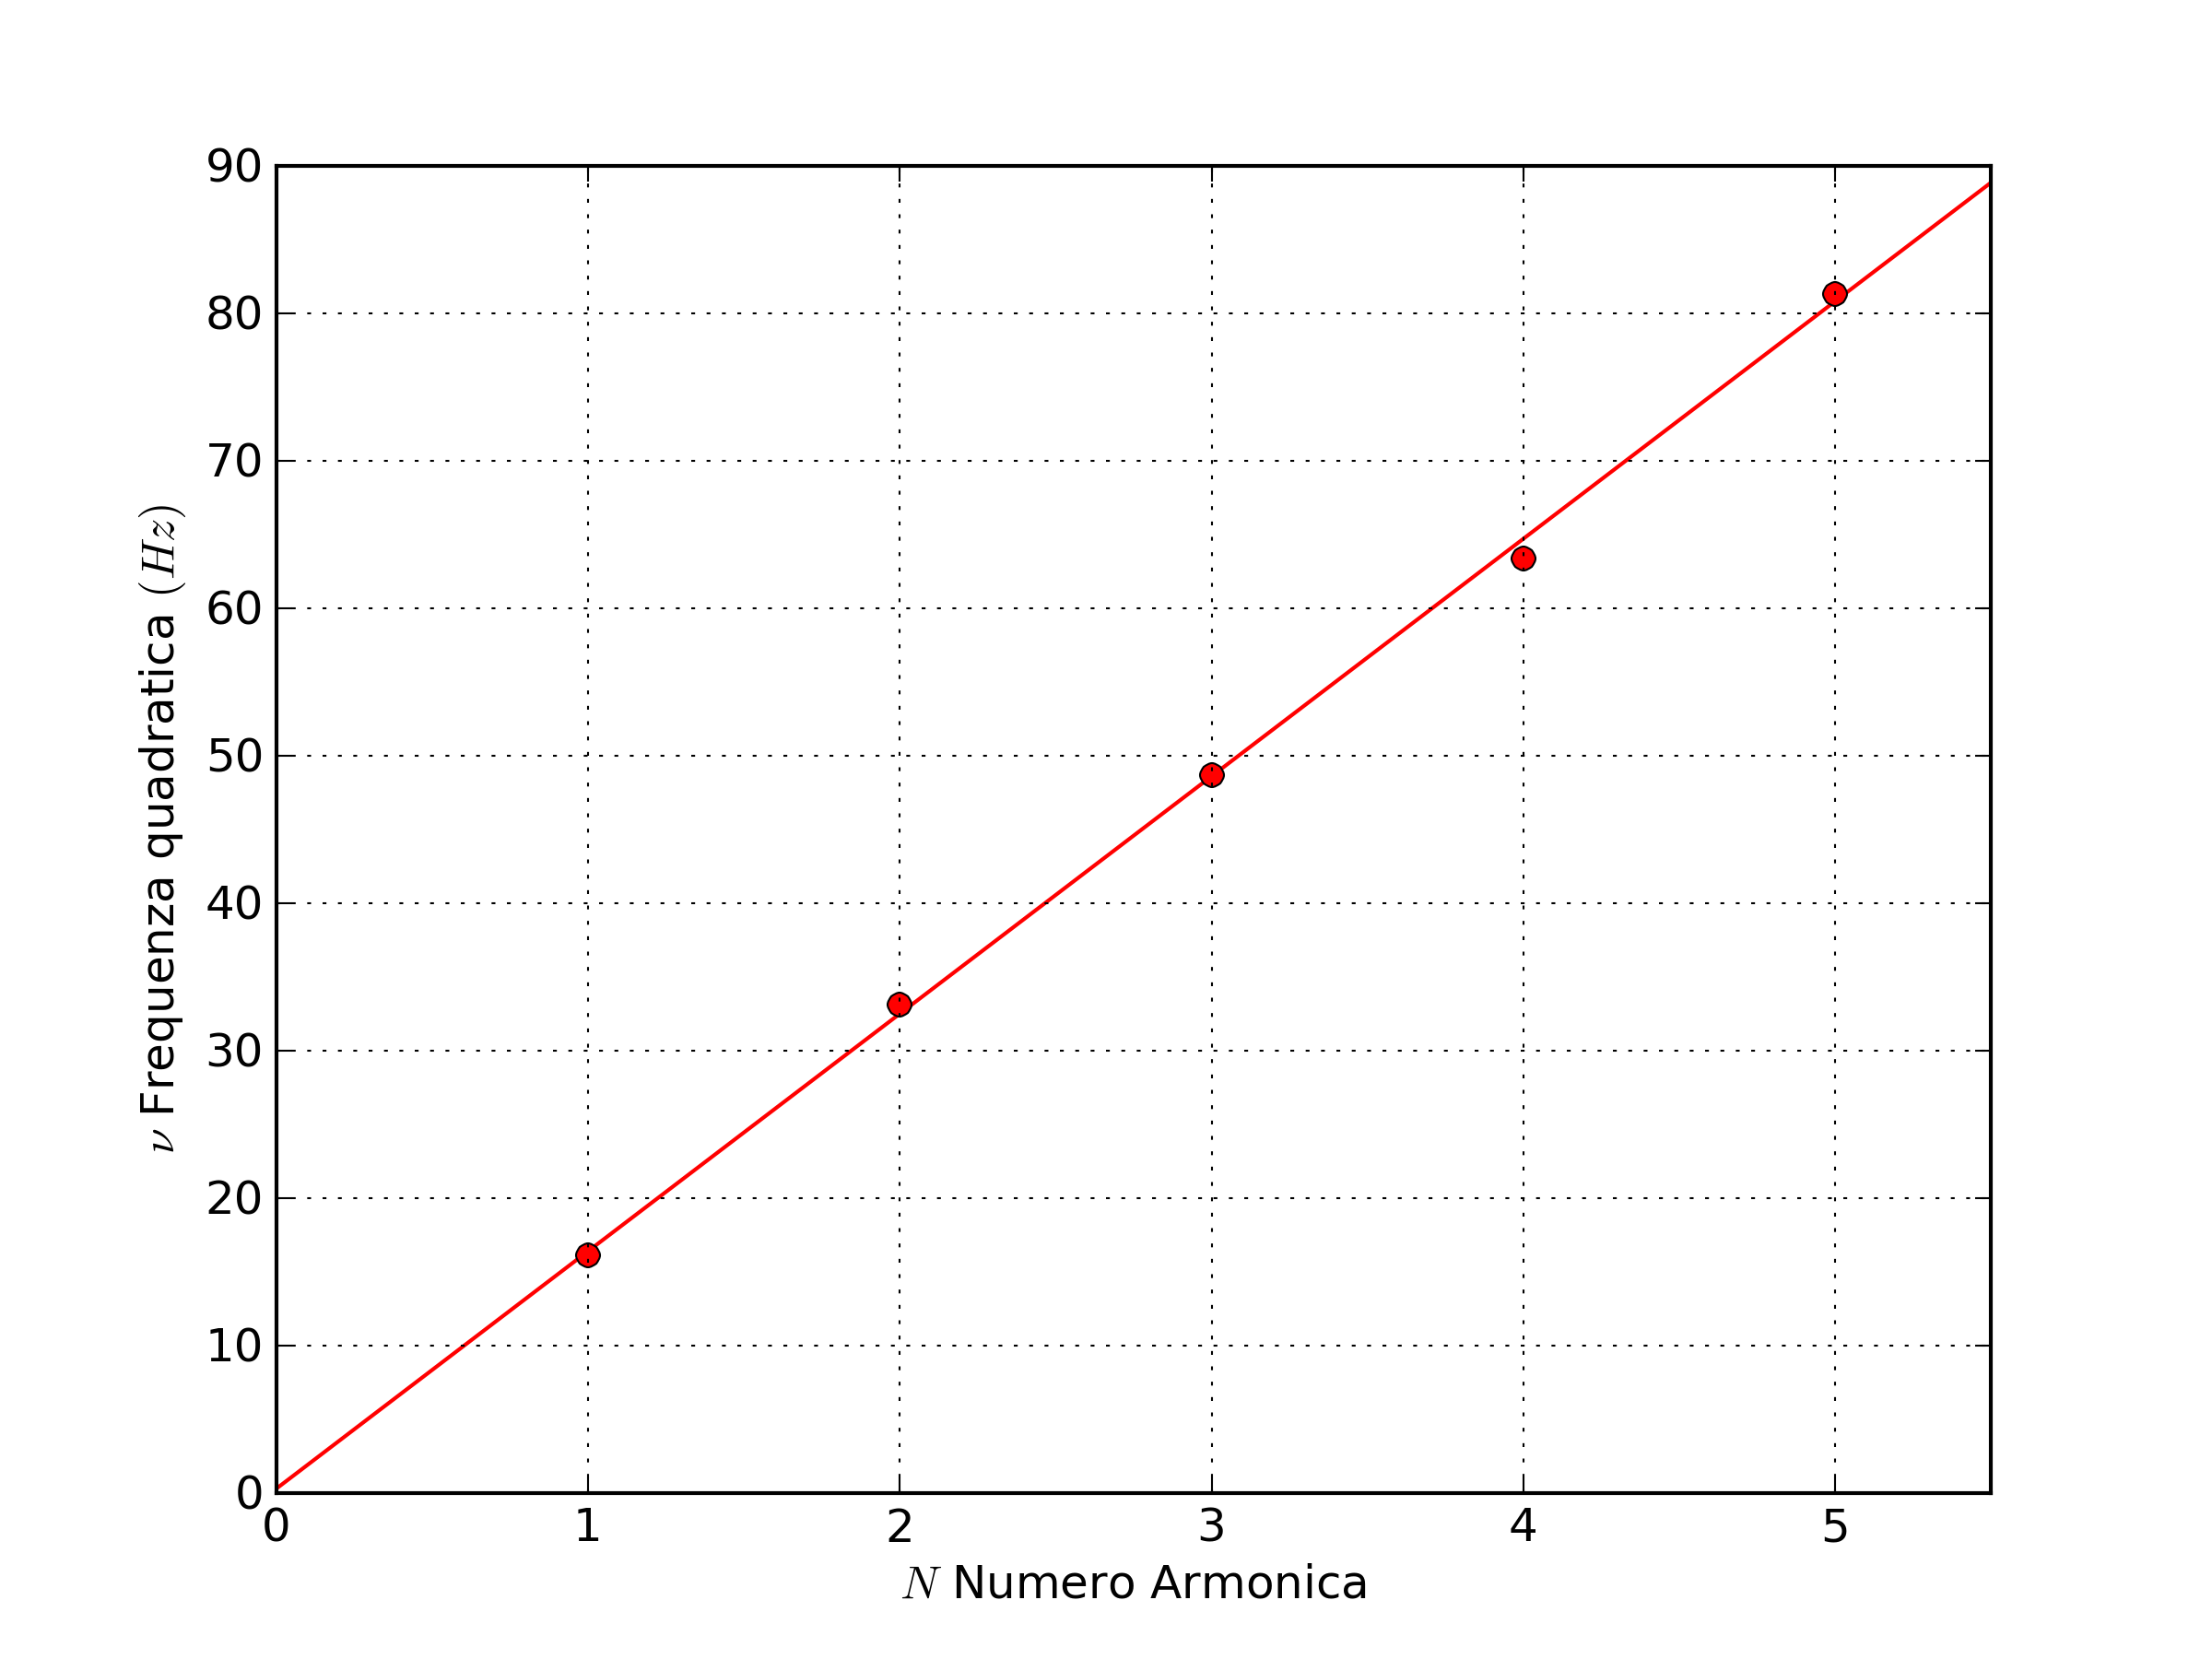
\includegraphics[scale=0.5]{../grafici/corda_1armonica}
\end{center}


\section{Dipendenza dalla tensione}
Dall'equazione $1.1$ si deduce la dipendenza quadratica tra la tensione $T$ e la frequenza $\nu$. 
Verifichiamo questa dipendenza utilizzando i dati della seconda armonica misurati precedentemente. 
\begin{center}
\begin{tabular}{c | c}

\textbf{Corda A}
\begin{tabular}{c|c}
Tensione $N$ & Frequenza $Hz$ \\
\midrule
2.45 & 33.1\\
3.43 & 37.8\\
4.41 &42.6\\
5.39 &45.6\\
\end{tabular}
&\textbf{
Corda B}
\begin{tabular}{c|c}
Tensione $N$ & Frequenza $Hz$ \\
\midrule
3.45 & 22.8\\
4.41 & 25.4\\
5.39 & 26.8\\
10.3 & 38.4\\
\end{tabular}
\\
\end{tabular}
\end{center}

Essendo il numero dei dati troppo ridotto per essere interpolato con successo dalla curva corrispondente ($1.1$), consideriamo un'interpolazione lineare di tipo $y = mx$ dove   $y= \nu^2$ e $x = T$.
\\
Utilizziamo il metodo dei minimi quadrati, ottenendo per la\textbf{ corda A} $m_A = 403.95$ con incertezza $\sigma_m =0.03$ e per la \textbf{corda B} $m_B=143.0$ con incertezza $\sigma_m$.  Di seguito il grafico che rappresenta la relazione tra $\nu^2$ e $T$.

\begin{center}
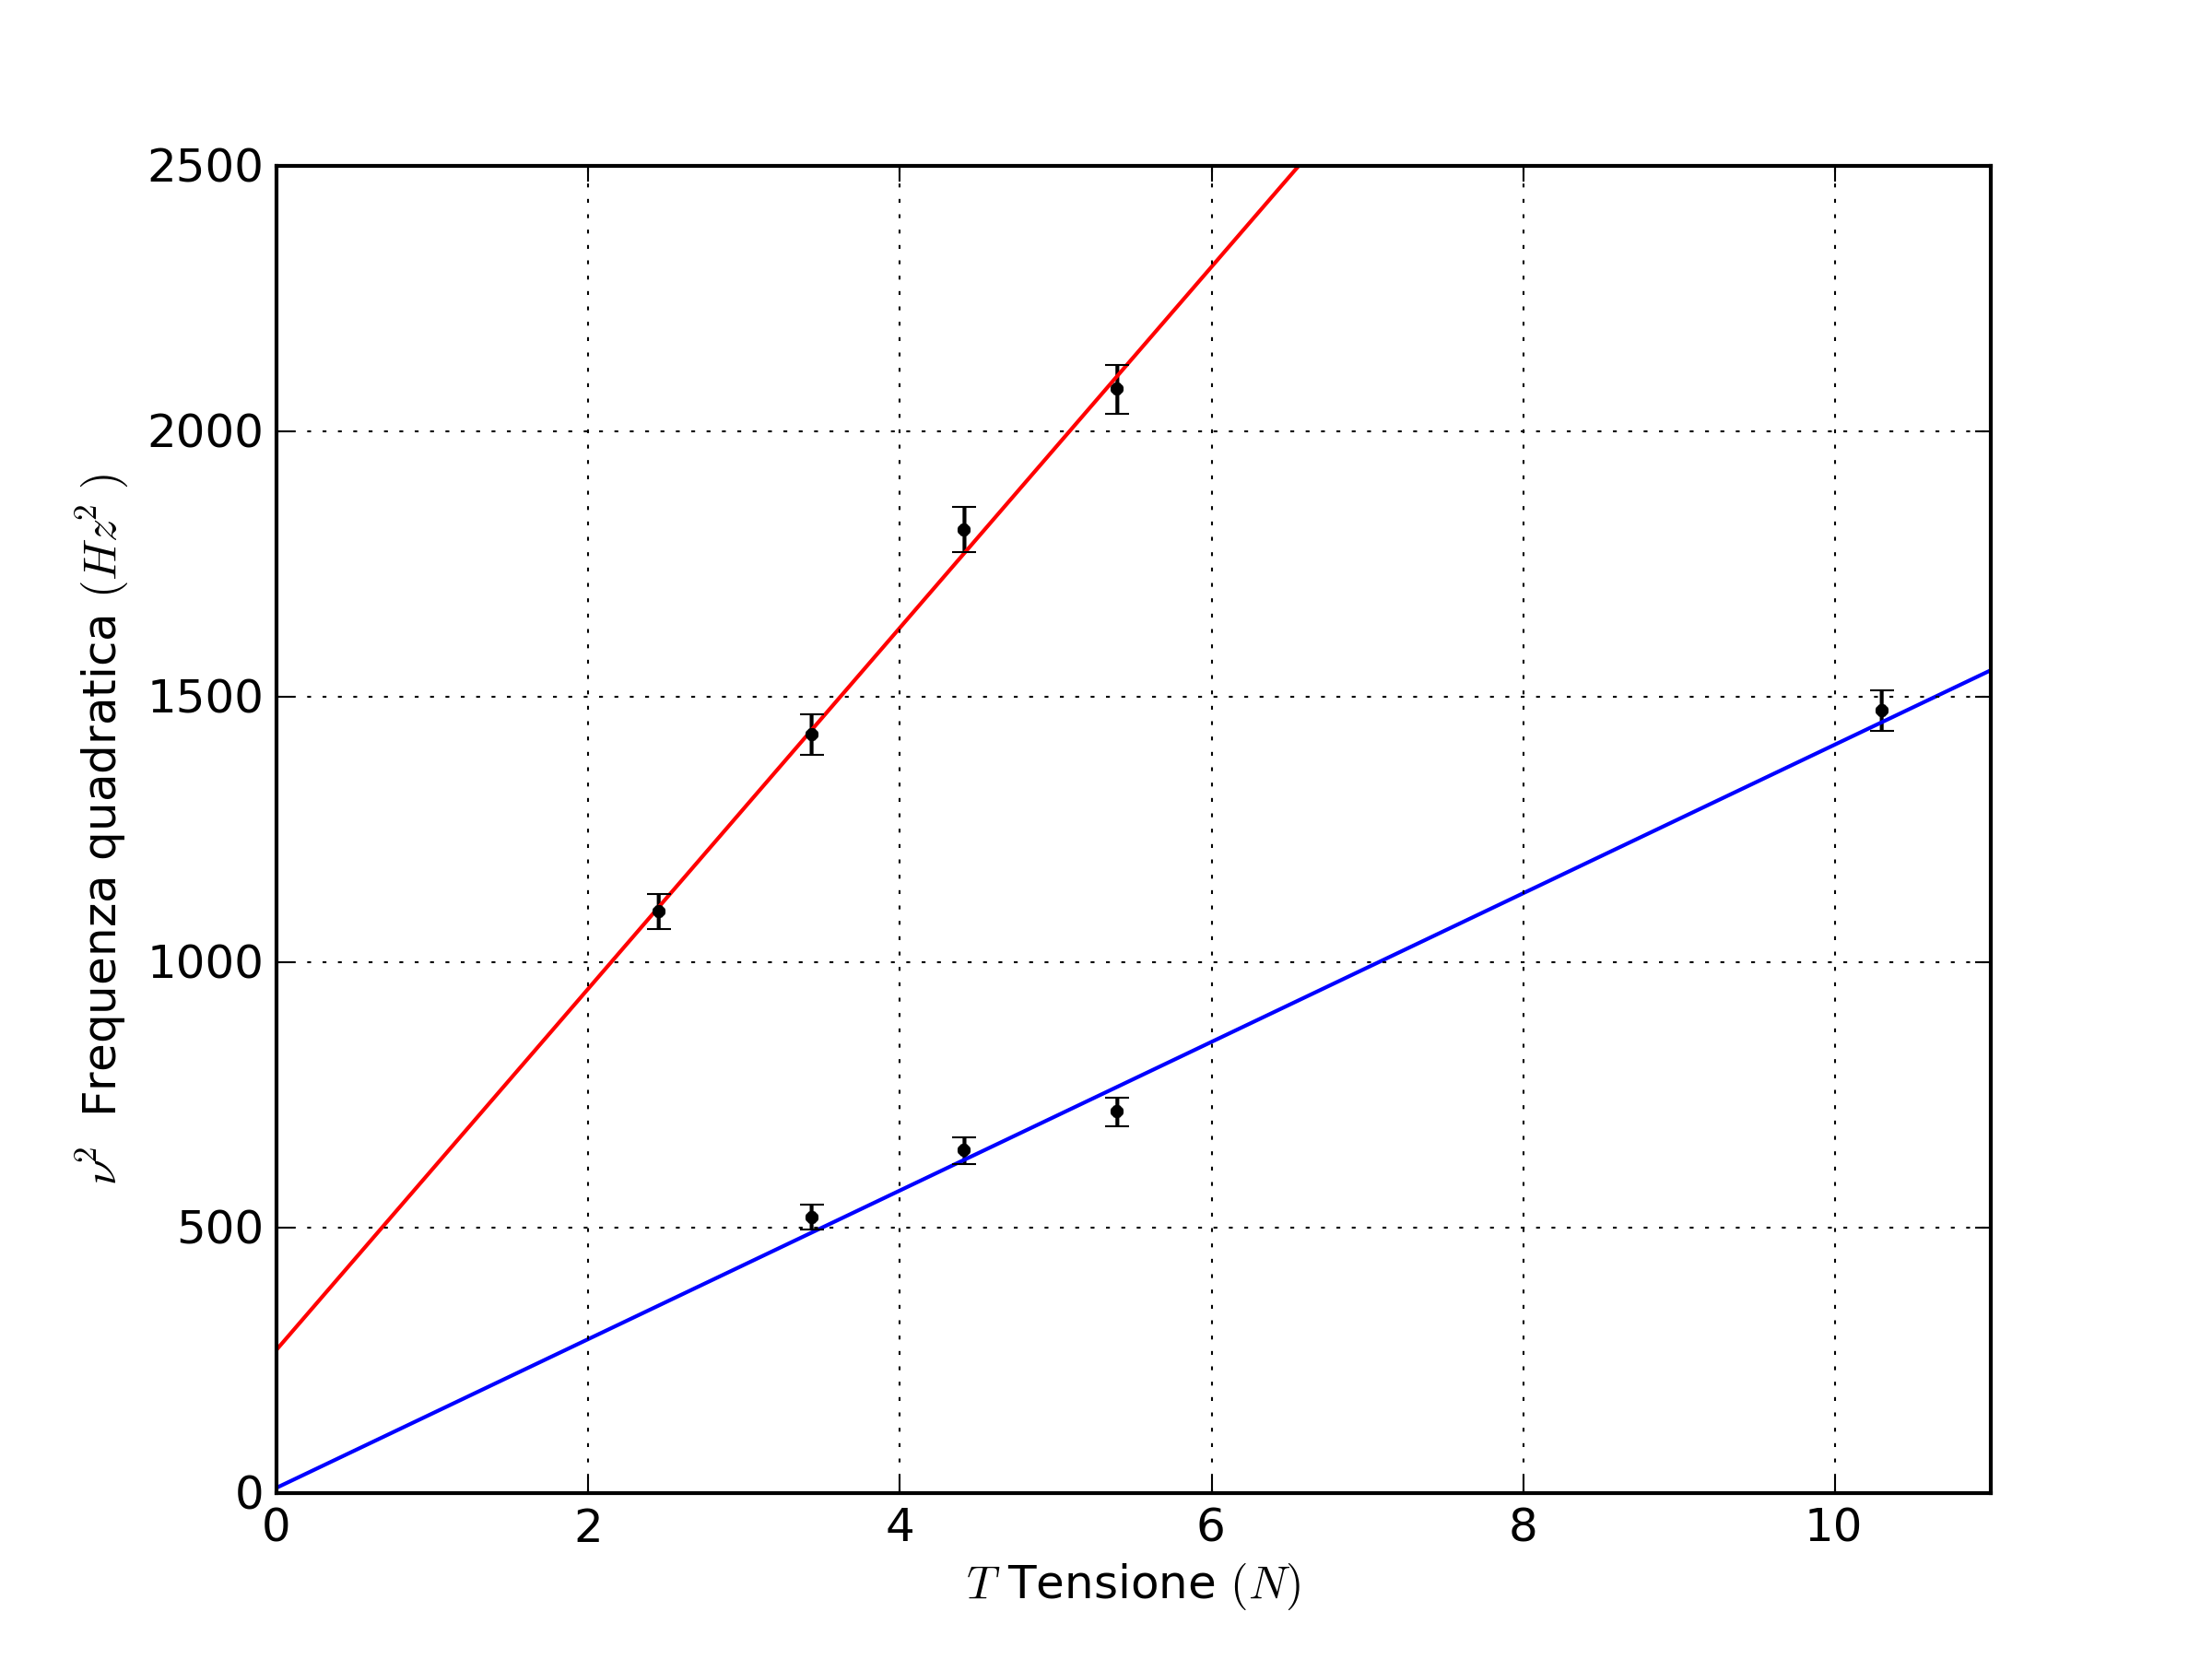
\includegraphics[scale=0.5]{../grafici/corda_tensione}
\end{center}



\section{Dipendenza dalla lunghezza}
L'ultima analisi riguarda la dipendeza di $\nu_n$ dalla lunghezza della corda, per una data tensione fissata. Essa è ancora una conseguenza della $1.1$, dalla quale si deduce che le due grandezze sono legate da proporzionalità inversa.\\
 
Di seguito sono riportati in tabella i valori raccolti per la prima armonica, per le corde A e B; sono stati scelti valori differenti per le due tensioni in quanto la corda a massa lineare maggiore aveva una risposta poco significativa quando soggetta alla tensione che si era usata per la corda A.\\

\begin{center}

\begin{tabular}{c c}

\textbf{Corda A},  $T=5.40\ N$ & \hspace{3cm} \textbf{Corda B},  $T=10.3\ N$\\
\\
\begin{tabular}{|c|c|}
\toprule
L($m$) & $\nu (Hz) $ \\
\midrule
1.05 & 24.6\\
1.11 & 23.7\\
1.17 & 22.8 \\
1.23 & 20.9 \\
1.32 & 20.1 \\
\bottomrule
\end{tabular}
 
& \hspace{3cm}

\begin{tabular}{|c|c|}
\toprule
L($m$) & $\nu (Hz) $ \\
\midrule
1.10 & 19.33 \\
1.15 & 18.25 \\
1.17 & 17.75 \\
1.22 & 17.00 \\
1.34 & 15.69 \\
1.53 & 13.92 \\
1.60 & 12.96 \\
0.91 & 22.83 \\
0.75 & 27.85 \\
0.60 & 35.00 \\
0.50 & 42.67 \\
\bottomrule
\end{tabular}

\end{tabular}

\end{center}



Il grafico seguente illustra il comportamento della corda B.

\includegraphics[scale=0.75]{"../grafici/CordaPrimaArmonica"}

Nota: $\rho$ è lasciato parametro libero, mentre $T$ è pari a 10.3 N, dato da un peso di 1.050 Kg sospeso a un'estremità della corda.



%
\section{Introduzione}
\subsection{Scopo dell'esperimento e metodo in breve}
L'esperimento si compone di tre parti.


Nella prima, si verifica la validità della Legge di Snell e la reversibilità del cammino ottico: dato un raggio luminoso attraversante un semi-cilindro in plexiglass, misuriamo l'angolo di incidenza $\theta_{rifrazione}$ ed il corrispondente  angolo di rifrazione $\theta_{rifrazione}$. Sempre grazie alla legge di Snell si ricerca la miglior stima dell'indice di rifrazione del plexiglass $n$.


Nella seconda parte, si ricerca $n$ studiando l'angolo di deviazione minima $\delta_{min}$ di un prisma a base triangolare e di un prisma a base trapezoidale. 
Inoltre, si ricerca la distanza di cui viene traslato il raggio, che arriva con un certo angolo di incidenza $\theta$, quando passa per due superfici parallele.


Infine si verifica la legge dei punti coniugati tramite la misura delle distanze $p$ e $q$ e la validità dell'ingrandimento ottico M. 

\subsection{Strumenti}
In questa tabella vengono riassunti gli strumenti rivelatori utilizzati, con le relative precisioni, e il set-up dell'esperimento.
\begin{center}
\begin{tabular}{c|c}
Strumento & Precisione \\
\midrule
Piatt. Graduata & $\pm 1 grado $ \\
Metro & $\pm 1 mm $\\
\end{tabular}
\end{center}


Durante l'esperimento è stato impostato sulla modalità a singolo raggio luminoso per le prime due parti e successivamente sulla modalità oggetto per la terza e ultima parte. 
Questo proiettore, insieme alla piattaforma girevole graduata, alle lenti ed a uno schermo bianco, può scorrere liberamente lungo una rotaia, permettendo di modificare le distanze tra gli oggetti a piacimento.
%Scherma dell'esperimento qui

\section{Reversibilità del cammino luminoso}
\subsection{Raccolta dati}
Tutte le misure seguenti sono espresse in gradi.


\begin{table}
\center
\begin{tabular}{c|c||c|c}
 \multicolumn{2}{c}{\textit{Faccia piana}} &
\multicolumn{2}{c}{\textit{Faccia curva}} \\
$\theta_{incidenza} $ & $\theta_{rifrazione} $ &$\theta_{incidenza} $ & $\theta_{rifrazione} $\\
\midrule
 10 & 7 & 7 & 10 \\
15 & 10 & &\\
20 & \textbf{13.5} & 13.5 & 20\\ 
25 & \textbf{16.5} & & \\
30 & 20 & 30 & 20\\
40 & 26 & 26 & 40\\
35 & 23 & &\\
45&  \textbf{28.5} & & \\
\end{tabular}
\caption*{Misure in gradi}
\end{table}

\subsection{Analisi dei dati}
Raccolti i valori degli angoli di incidenza e dei corrispondenti angoli di rifrazione, possiamo calcolare la miglior stima di $n$.
La legge di Snell esprime la relazione che lega gli indici di rifrazione dei due materiali attraversati dal raggio luminoso, e i seni degli angoli di incidenza e rifrazione:

\begin{center}
$n_1 sin\theta_1 = n_2 sin\theta_2$
\end{center}

Poiché $n_a \simeq1 $ ( indice di rifrazione dell'aria ), si ricava:

$$n_2 = \frac{sin\theta_1}{sin\theta_2}$$

Nell'elaborazione dei dati, abbiamo selezionato solo le coppie di misure cui corrispondesse un errore relativo percentuale minore del 6\%, al fine di avere una stima più precisa del valore vero di $n$.

\begin{center}
\begin{tabular}{c|c|c|c|c|c}
\textbf{$\theta_1$} & 25 & 30 & 40 & 35 & 45\\
\midrule
\textbf{$\theta_2$} & 16.5 & 20 & 26 & 23 & 28.5\\
\midrule
\textbf{$n_i$} (*) & 1.489 & 1.462 & 1.468 & 1.468 & 1.482\\
\end{tabular}\\

\end{center}
(*) in questo caso abbiamo tenuto un numero superiore di cifre significative, in quanto si tratta di calcoli intermedi 
%Ripensare alle cifre significative

$$\overline{n} = \frac{\displaystyle\sum\limits_{i=1}^N n_i}{N} = 1.474 $$

$$\sigma_n = \sqrt{\frac{\sum_{i=1}^N n_i}{N-1}} = 0.01$$

$$\sigma_{\overline{n}} = \frac{\sigma_n}{\sqrt{N}} = 0.004$$

$$n_{best} = 1.474  \pm 0.004 $$

%Cifre significative incertezza diverse da cifre significative misura!

\section{Misura dell'angolo di deviazione minima}
\subsection{Raccolta dati}

L'angolo di deviazione minima ($\delta_{min}$) è il più piccolo angolo misurato facendo incidere un fascio di luce su una faccia di prisma (con inclinazione variabile) e misurando l'ampiezza dell'angolo rifratto. Nel nostro esperimento abbiamo utilizzato due prismi: uno con base un triangolo equilatero e l'altro un trapezio rettangolo.

In tabella sono riportati i valori trovati per ogni misurazione dell'angolo rifratto. Per aumentare il livello di precisione, abbiamo raccolto i dati relativi agli angoli di deviazione minima per ogni faccia di prisma a base triangolare, identificando ogni misurazione con il numero dello spigolo compreso tra le facce colpite e il verso di percorrenza della luce.

Per ovvie ragioni geometriche, nel caso del prisma a base trapezoidale (è presente un solo angolo acuto, di 45 gradi) è stato impossibile effettuare misure riferite a vari vertici.

\begin{table}
\center
\renewcommand{\arraystretch}{1.2}
\begin{tabular}{|c | c | c|}
\hline
Spigolo & $\delta_{min}$ (andata) & $\delta_{min}$ (ritorno)\\
\hline
\multicolumn{3}{|c|}{\textit{Prisma a base triangolare}} \\
\hline
1 & 41 & 31\\
2 & 43 & 39\\
3 & 41 & 41\\
\hline
\multicolumn{3}{|c|}{\textit{Prisma a base trapezoidale}} \\
\hline
1 & 28 & 21\\
\hline
\end{tabular}
\end{table}

$\overline{\delta}_{min} = \frac{\displaystyle\sum\limits_{i=1}^6 \delta_i}{6} = 1.52$

%Angolo deviazione minima, immagine
\subsection{Analisi dei dati}

\section{Lenti sottili}
\subsection{Raccolta dati}
Nell'ultima parte dell'esperimento, si verifica la validità della legge dei punti coniugati,
$$ \frac{1}{f} = \frac{1}{q} + \frac{1}{p} $$
\textit{p: distanza sorgente-lente}
\textit{q: distanza lente-schermo}
\textit{d: diametro circonferenza proiettata}

In tabella sono riportati sulla destra le misure effettuate con lente di focale $f=100 mm$, a sinistra con lente di focale $f=200mm$. Tutti i valori sono in cm.

\begin{center}
\begin{tabular}{*{3}{c|}*{3}{|c}}
p & q &d &p &q&d\\
\midrule
13.5 & 36.5 & 5.5 & 73.4 & 26.6 & 0.7\\
36.2 & 13.8 & 0.8 & 26.4 & 73.6 & 5.5\\
\midrule
18.0 & 22.0 & 2.5 & 61.5 & 28.5 & 0.9\\
22.0 & 18.0 & 2.1 & 28.1 & 61.9 & 4.8\\
\end{tabular}
\end{center}

Inserire propagazione degli errori. 
\subsection{Analisi dei dati}
Per verificare la validità, rappresentare su un grafico i punti ($\frac{1}{p};\frac{1}{q})$ e verificare che i punti sono disposti lungo una retta. 
Calcolo l'incertezza $\sigma_{q}$ e $\sigma_{p}$, tramite la Dev. Std. 

%Grafico delle due rette


\section{Conclusioni}







\chapter*{Appendice}
\section*{Metodo di analisi dei dati informatizzato}
Per l'analisi dei dati sperimentali si è fatto largo uso di strumenti informatici ausiliari.
In particolare, è stata usata l'applicazione DataStudio per la raccolta di dati da sensori elettronici, ed occasionalmente per l'interpolazione dei dati.
Per quanto riguarda l'analisi degli errori, si è preferita una soluzione costruita tramite il pacchetto software open source "Sage", distribuito sotto i termini della GNU General Public License.

Questo strumento utilizza il linguaggio di programmazione Python, e alcune librerie esterne. Di seguito viene allegato e commentato il programma principale, scritto da noi.

\begin{lstlisting}
reset()

format = "png"
dpis = 90

import numpy as np
import matplotlib.pyplot as plt
\end{lstlisting}

Questa sezione è un preambolo: vengono importate le librerie principali, viene impostato il formato di output desiderato (in questo caso "png", comodo per lo sviluppo) e la risoluzione di questo output.

\begin{lstlisting}
class Analyzer:
    uuid = "" # internally used
    caption = "" # caption for the histogram/plot
    color = '#50e300' # histogram color
    nOfBins = 5; # number of bins (default: 5)
    data = [] # array with data. if you're using integer values,
    		  # make sure at least one is a float.
    x = "" # x-axis label, latex syntax
    y = "" # y-axis label, latex syntax
    
    plotText = "" # optional: print this text on the plot - latex syntax
    xUnitOfMeasure = "" # optional: unit of measure of x
    
\end{lstlisting}

Questa è la classe base: si occupa di disegnare il grafico e di fornire l'analisi statistica di base

\begin{lstlisting}
    def setTitle(self, caption):
        self.caption = caption
        self.uuid = caption.replace('\\', '').replace(' ', '')
        
    # Note: make sure xUnitOfMeasure is set before calling this
    def quickPrepare(self, list):
        m = self.xUnitOfMeasure
        self.y = "f(k)/\\Delta k"
        self.data = list['data']
        self.setTitle(d['uuid'])
        if('bins' in d):
            self.nOfBins = d['bins']
        self.plotText = '\mu = %.5f %s;\ \sigma = %.5f %s;'\
                        % (mean(self.data), m, std(self.data), m)
        
    def plotGauss(self):
        a = self.data
        
        plt.clf()
        mu = mean(a)
        sigma = std(a)
        n, bins, patches = plt.hist(a, self.nOfBins, normed=1, facecolor=self.color, alpha=0.75)
        
        x = np.arange(min(bins)-10*sigma, max(bins)+10*sigma, 0.02*(max(bins)-min(bins)));
        y = 1/(sigma*np.sqrt(2*np.pi)) * np.exp( -((x-mu)^2 / (2* (sigma^2) )) );
        l = plt.plot(x, y, 'k--', linewidth=1)
        
        plt.xlabel(r"$"+self.x+"$")
        plt.ylabel(r"$"+self.y+"$")
        
        plt.title(r"$"+self.caption.replace(' ', '\\ ')+"$")
        plt.axis([mu-3*sigma, mu+3*sigma, 0, 3/(sigma*np.sqrt(2*np.pi))])
        
        plt.annotate(r"$"+self.plotText+"$", xy=(0.075,0.85), xycoords='axes fraction')
        
        plt.grid(True)
        plt.savefig(self.uuid+"."+format, dpi=dpis)
        
    def statAnalysis(self):
        stderr = "%.5f" % (std(self.data)/np.sqrt(len(self.data)))
        media = "%.5f" % mean(self.data)
        stddev = "%.5f" % std(self.data)
        print "=== "+self.caption+" ==="
        print "Media: "+ media +" - Std. Dev.: "+ stddev
        print "Errore della media: "+ stderr
\end{lstlisting}

\end{document} 



